\documentclass[12pt, openright, twoside]{book}

% ---------------------------------------------------------------
% Engine and font setup (XeLaTeX / LuaLaTeX compatible)
% ---------------------------------------------------------------
\usepackage{fontspec}
\usepackage{unicode-math}
\setmainfont{TeX Gyre Pagella}
\setmathfont{Latin Modern Math}
\usepackage[english]{babel}

% ---------------------------------------------------------------
% Page geometry
% ---------------------------------------------------------------
\usepackage[
  paperwidth=6in,
  paperheight=9in,
  top=1in,
  bottom=1in,
  inner=1.1in,
  outer=0.85in,
  headsep=14pt
]{geometry}

% ---------------------------------------------------------------
% Typography
% ---------------------------------------------------------------
\usepackage{microtype}
\usepackage{setspace}
\setstretch{1.15}
\usepackage{parskip}
\setlength{\parindent}{0pt}
\setlength{\parskip}{6pt plus 2pt minus 1pt}

% ---------------------------------------------------------------
% Running heads
% ---------------------------------------------------------------
\usepackage{fancyhdr}
\setlength{\headheight}{14pt}
\pagestyle{fancy}
\fancyhf{}
\fancyhead[LE]{\small\itshape The Collapse of Epistemic Coherence}
\fancyhead[RO]{\small\itshape\leftmark}
\fancyfoot[C]{\small\thepage}
\renewcommand{\headrulewidth}{0.4pt}
\fancypagestyle{plain}{%
  \fancyhf{}%
  \fancyfoot[C]{\small\thepage}%
  \renewcommand{\headrulewidth}{0pt}%
}

% ---------------------------------------------------------------
% Chapter and section titles
% ---------------------------------------------------------------
\usepackage{titlesec}
\titleformat{\chapter}[display]
  {\normalfont\large\bfseries}
  {\chaptertitlename\ \thechapter}
  {10pt}
  {\LARGE}
\titlespacing*{\chapter}{0pt}{30pt}{20pt}

\titleformat{\section}
  {\normalfont\large\bfseries}
  {\thesection}{1em}{}
\titlespacing*{\section}{0pt}{18pt}{6pt}

\titleformat{\subsection}
  {\normalfont\normalsize\bfseries}
  {\thesubsection}{1em}{}
\titlespacing*{\subsection}{0pt}{12pt}{4pt}

% ---------------------------------------------------------------
% Technical Note boxes
% ---------------------------------------------------------------
\usepackage[most]{tcolorbox}
\tcbuselibrary{breakable}
\newtcolorbox{technicalnote}[1][]{%
  breakable,
  enhanced,
  colback=gray!6,
  colframe=gray!40,
  boxrule=0.4pt,
  arc=2pt,
  left=8pt, right=8pt, top=6pt, bottom=6pt,
  fonttitle=\small\bfseries\itshape,
  title={Technical Note},
  #1
}

\usepackage{graphicx}
\usepackage{caption}
\usepackage{subcaption}
\graphicspath{{./figures/}{./}}

% ---------------------------------------------------------------
% Mathematics
% ---------------------------------------------------------------
\usepackage{amsmath}

% ---------------------------------------------------------------
% Quotations
% ---------------------------------------------------------------
\usepackage{csquotes}

% ---------------------------------------------------------------
% Bookmarks
\PassOptionsToPackage{hidelinks,
  pdfauthor={Flyxion},
  pdftitle={The Collapse of Epistemic Coherence},
  pdfsubject={Epistemology, Philosophy of Science, Language Models}
}{hyperref}
\usepackage{bookmark}


% ---------------------------------------------------------------
% Table of contents depth
% ---------------------------------------------------------------
\setcounter{tocdepth}{1}

% ---------------------------------------------------------------
% Metadata
% ---------------------------------------------------------------
\title{\textbf{The Collapse of Epistemic Coherence}\\[8pt]
\large Language Models, Synthetic Formalism,\\
and the Industrialization of Intellectual Atmosphere}
\author{Flyxion}
\date{2026}

\begin{document}

\frontmatter

% ----- Half-title page -----------------------------------------
\begin{titlepage}
\centering
\vspace*{3cm}
{\Huge\bfseries The Collapse of Epistemic Coherence\par}
\vspace{1.2cm}
{\Large Language Models, Synthetic Formalism,\\[4pt]
and the Industrialization of Intellectual Atmosphere\par}
\vfill
{\large Flyxion\par}
\vspace{0.5cm}
{\normalsize Independent Researcher\par}
\vspace{2cm}
{\normalsize 2026\par}
\end{titlepage}

% ----- Copyright page ------------------------------------------
\thispagestyle{empty}
\vspace*{\fill}
\noindent
\textcopyright\ 2026 Flyxion.\\[4pt]
All rights reserved. No part of this publication may be reproduced,
distributed, or transmitted in any form or by any means without the
prior written permission of the author, except for brief quotations
in critical reviews and scholarly commentary.\\[12pt]
\noindent
\textit{First edition, 2026.}
\vspace*{\fill}
\newpage

% ----- Table of contents ---------------------------------------
\tableofcontents
\clearpage

\mainmatter

\chapter*{Preface}

\section*{On Writing During the Generative Transition}

This book was written using the systems it critiques. That sentence is not a confession
of inconsistency but a statement of method. Any serious attempt to understand the
epistemic dynamics of generative language systems must proceed from within those
dynamics, not from a position of imagined exemption. The philosopher who studies
optical illusions cannot see through them by force of will; what changes is only the
precision with which the illusion is understood. The situation here is structurally
similar, and the analogy is more than decorative. Generative language systems alter
the conditions of intellectual production in ways that affect everyone who writes,
reads, or reasons inside environments saturated with their outputs---which is now,
effectively, everyone.

The first thing this book is not is an argument against abstraction. Cross-domain
synthesis, formal modeling, speculative theory, and systematic philosophy are not
pathologies; they are among the most powerful intellectual instruments civilization
has developed. The capacity to perceive structural similarity across apparently
unrelated domains has produced thermodynamics, information theory, evolutionary
biology, and the foundations of modern logic. Nothing in these pages should be read
as a defense of disciplinary parochialism or a complaint that ideas have become too
ambitious. The argument is more specific and, the author believes, more troubling than
that.

What this book argues is that we are living through a structural transition in the
ecology of knowledge production---one in which semantic coherence has become
industrially reproducible at scales that far exceed our collective capacity to audit
inferential integrity. This distinction, between semantic coherence and inferential
integrity, is the central conceptual axis of everything that follows, and it is
worth stating plainly at the outset.

Semantic coherence is a surface property. A text possesses it when its sentences flow
naturally into one another, when its vocabulary is internally consistent, when its
transitions feel motivated, and when its conclusions seem to follow from its
premises. Inferential integrity is a deeper property. A text possesses it when
its conclusions actually follow from its premises through steps that can be traced,
checked, and in principle contested; when its formal structures do real constraining
work on interpretation rather than merely decorating prose; when its observational
claims are distinguishable from its definitional stipulations; and when it exposes
the conditions under which it could be wrong. These two properties frequently
coincide in good intellectual work. The problem this book addresses is that they
are increasingly separable, and that the systems now industrializing intellectual
production are optimized almost exclusively for the former.

Modern generative language systems preserve symbolic continuity with extraordinary
fidelity. A well-prompted language model will maintain consistent vocabulary,
sustain appropriate register, connect clauses with plausible transitions, and
produce conclusions that feel earned. What such systems cannot reliably preserve
is inferential continuity---the chain of constraint that prevents a formal symbol
from meaning anything the prose subsequently requires it to mean. This divergence
is not primarily a technical limitation awaiting resolution in the next model
generation. It reflects a structural feature of how these systems are trained and
what they are optimized to produce. They are, at their core, continuation engines:
given a semantic context, they extend it in ways that preserve its surface
properties. Truth, in the sense of correspondence to external structure, is only
weakly coupled to that objective. Inferential validity is more weakly coupled still.

The consequences of this divergence are already visible and are accelerating. They
manifest not as obvious falsehood---the hallucinated citation, the invented
statistic, the plain factual error---but as something more epistemically insidious:
a flattening of reliability gradients across texts that are superficially
indistinguishable. A careful empirical study and a sophisticated-sounding framework
that merely redescribes what it claims to explain can now be made to look, at the
level of surface structure, almost identical. This is not because the careful study
has become worse. It is because the cost of producing the sophisticated-sounding
framework has collapsed toward zero. The problem is not the existence of weak
intellectual work---that is not new---but the change in its relative density inside
the epistemic environment. When synthetic coherence is industrially producible,
genuine inferential rigor does not become rarer in absolute terms; it becomes
statistically harder to locate. Truth signals weaken not because truth disappears
but because the noise floor rises.

It would be a serious misreading to conclude from this that language models have
caused the situation. Synthetic formalism---the production of frameworks that
marshal the aesthetic authority of mathematics and formal philosophy while
systematically evacuating their operational content---predates generative AI by
decades. Its precursors can be traced through postmodern academic opacity, through
the universalizing ambitions of first-generation cybernetics, through the more
extravagant branches of speculative continental philosophy, through pop complexity
science and its enthusiasm for fractals and emergence as universal explanatory
currency, through New Age physics, through corporate futurism, and through what
might be called the TED-talk synthesis culture of the early twenty-first century:
the production of large, confident, cross-domain claims whose appeal derives almost
entirely from their narrative fluency rather than their inferential content.
What language models have done is remove the production bottlenecks that previously
limited this tendency's scale. Writing synthetic philosophy at high quality---meaning
high surface quality, the quality of tone and coherence and apparent depth---
previously required real effort and some threshold of domain knowledge. That
threshold created friction, and friction, whatever its costs, is also a filter.
The filter was always imperfect, but it existed. What we are now witnessing is the
removal of that filter while leaving in place all the social and institutional
mechanisms that reward its outputs.

The argument of this book therefore has three distinct registers that the reader
should keep simultaneously in view. The first is diagnostic: what are the specific
failure geometries of synthetic formalism, and how do they recur across apparently
unrelated intellectual contexts? The second is structural: how has the industrialization
of these failure geometries transformed the epistemic environment in which all
intellectual work now takes place? The third is constructive: what practices, norms,
and institutional forms could restore inferential integrity as a legible and
socially rewarded property of intellectual production?

A note on the case studies in Part~IV is necessary here. This book examines several
bodies of theoretical work in some detail. That examination is critical, sometimes
severely so. The author wishes to be precise about what those criticisms are and
what they are not. They are not arguments that the researchers in question are
incompetent, dishonest, or intellectually unserious. The failure modes described
in this book are seductive precisely because they are available to anyone working
under the pressures---toward novelty, toward synthesis, toward cross-domain
ambition---that the contemporary intellectual environment creates and rewards.
Crucially, these failure modes are available to the author as well. The frameworks
the author has developed---the RSVP field system, the Spherepop event calculus,
the TARTAN coarse-graining architecture---are not presented here as exemplars of
inferential rigor. They are presented as frameworks that attempt certain kinds of
discipline while remaining genuinely vulnerable to many of the pathologies this
book describes. Appendix~D is devoted to an explicit audit of those vulnerabilities.
That audit is not false modesty; it is a methodological requirement. A book about
the failure modes of synthetic formalism that presents its own theoretical apparatus
as exempt from those failure modes would be a self-refuting document.

The reflexive character of this project runs deeper still. This book was composed
partly through extended dialogue with generative language systems. Significant
portions of its argumentative structure emerged through that dialogue. The author
has attempted to audit those dialogues for exactly the pathologies described
here---sycophantic reinforcement of the author's prior commitments, narrative
completion dynamics that produce conclusions not actually entailed by premises,
the generation of vocabulary that sounds precise while remaining operationally
underdetermined. Whether that audit has been fully successful is not something the
author can certify from inside the process. The reader who finds moments where
the book's own prose drifts from inferential to merely symbolic continuity is
not misreading; they may be observing the phenomenon in its natural habitat.
That possibility is not an embarrassment the author is trying to conceal but a
structural feature of intellectual work during the generative transition---work
that cannot be conducted from outside the systems transforming it.

One further self-imposed constraint should be made explicit. A critique of semantic
inflation must itself resist the temptation toward semantic totalization. The
argument that synthetic coherence is dangerous has a pathological attractor:
a theory of everything that explains every intellectual failure as an instance of
the same underlying dynamic, that produces a universal vocabulary of collapse and
drift and totalization, and that thereby demonstrates its thesis by becoming an
example of it. The author has tried to resist this attractor by maintaining the
length of the monograph within bounds that the argument actually requires, by
preserving specific and falsifiable claims wherever possible, and by marking the
limits of what the proposed framework can explain rather than expanding those
limits to cover everything. Whether these attempts succeed is, again, not something
the author can determine from inside the project. But the attempt is deliberate,
and naming it here creates at minimum a form of accountability.

The pages that follow are organized to move from diagnosis to structure to
consequence to reconstruction. Part~I establishes the historical genealogy of
synthetic formalism and its relationship to the current generative transition.
Part~II develops the conceptual vocabulary for analyzing the specific failure
geometries that recur across contexts. Part~III examines the mechanisms by which
language models function as accelerants of those failure geometries. Part~IV
presents the case studies. Part~V proposes audit protocols for distinguishing
inferential from symbolic continuity. Part~VI draws the philosophical consequences
of treating the current moment as a structural transition rather than a temporary
aberration. The appendices provide taxonomic and technical material that would
have interrupted the main argument.

The situation this book describes is not hopeless. Inferential integrity is not
a relic of a pre-digital epistemic order that generative systems have simply
terminated. It is a practice---difficult, always incomplete, requiring institutional
support and cultural reward---that the current transition makes harder but not
impossible. The constructive horizon toward which the final chapters gesture is
real: provenance-aware knowledge systems, adversarial auditing cultures, explicit
uncertainty grammars, simulation-linked theory development, and above all a renewed
commitment to the unglamorous virtues of partial understanding, exposed limitation,
and derivational transparency. These are not sufficient conditions for epistemic
health under generative pressure. They may be necessary ones. The difference
between those two claims is itself an instance of the kind of precision this book
is trying to practice.

\bigskip
\noindent\textit{Flyxion}\\
\noindent\textit{Independent researcher}\\
\noindent\textit{Canada, 2026}

\clearpage

\part{The New Epistemic Environment}

\chapter{The End of Epistemic Scarcity}

\section{A History of Coupling Mechanisms}

The argument of the previous chapter established a distinction between two
properties of reasoning: symbolic continuity and inferential continuity. It
established further that human cognition treats the former as a proxy for the
latter, that this treatment has historically been adaptive, and that the
adaptive value of the proxy depends on an environmental condition --- a
sufficiently stable correlation between the two properties --- that can in
principle be disrupted. This chapter traces the historical mechanisms that
maintained that correlation and the sequence of transitions through which
those mechanisms have progressively weakened.

The governing question is not whether intellectual culture has declined. That
framing is both too moralistic and too imprecise to be useful. The question is
structural: what features of different historical environments served to keep
symbolic continuity and inferential continuity coupled, and how have changes
in those environments altered the coupling ratio? The answer that emerges is
not a narrative of decline but a story about the relationship between production
costs, audit capacity, and the social architecture of epistemic trust --- a
relationship that has remained broadly stable across many information
transitions and is now, for reasons specific to the generative moment, becoming
genuinely unstable for the first time.

The central claim of this chapter can be stated as follows. Throughout most of
the history of organized intellectual production, the costs of generating
symbolically coherent theoretical prose were high enough, and the social
mechanisms for evaluating that prose were well-coupled enough to the underlying
inferential properties, that the epistemic environment maintained a rough
equilibrium between symbolic production and inferential auditing. That
equilibrium was never perfect, was always contested, and produced its own
characteristic failure modes. But it was an equilibrium. What the generative
transition represents is not another perturbation within that equilibrium but
a shift in the underlying parameters that made equilibrium possible: specifically,
a collapse in the cost of symbolic production with no corresponding change in
the biological and institutional constraints on inferential verification. The
result is a new regime in which symbolic generation capacity has come to
dramatically exceed inferential audit capacity --- a regime whose consequences
are only beginning to be understood.

\section{Epistemic Coupling Mechanisms and Legitimacy Signals}

Before tracing the historical arc, it is necessary to introduce a distinction
that will carry weight throughout this book: the difference between epistemic
coupling mechanisms and epistemic legitimacy signals.

An epistemic coupling mechanism is any feature of an intellectual environment
that tends, through its operation, to keep symbolic continuity and inferential
continuity correlated. It need not do so intentionally or by design; many of
the most effective coupling mechanisms were structural byproducts of
institutional arrangements whose primary purposes were quite different. The
cost of manuscript copying, for instance, was a coupling mechanism not because
anyone designed it to function as one but because the expense of producing and
circulating long texts created selection pressure for texts whose intellectual
content could justify that expense --- and justifying that expense required,
in practice, that the texts actually demonstrate what they claimed to
demonstrate. The friction was incidental; the coupling was real.

An epistemic legitimacy signal, by contrast, is any feature of an intellectual
product that social systems use as evidence of inferential quality. Legitimacy
signals include: institutional affiliation, which is treated as evidence that
an author has undergone training sufficient to produce rigorous work; peer
review, which is treated as evidence that the work has been checked by
competent evaluators; mathematical notation, which is treated as evidence of
formal precision; citation density, which is treated as evidence of engagement
with the relevant literature; long-form argument, which is treated as evidence
of sustained analytical effort; and technical vocabulary, which is treated as
evidence of domain expertise. These signals are all, in the relevant historical
contexts, genuinely informative --- but they are informative because, and only
insofar as, they are correlated with underlying coupling mechanisms that make
their presence evidence of inferential quality.

The critical observation is this: legitimacy signals and coupling mechanisms
can come apart. When they do, legitimacy signals become reproducible
independently of the inferential discipline they were originally taken to
indicate. The surface of scholarly credibility remains intact while its
inferential substrate weakens. This decoupling of signals from mechanisms is
not a novel phenomenon --- it has occurred locally throughout intellectual
history, producing the various genres of learned-sounding empty writing that
every scholarly tradition has generated. What is novel about the current moment
is that the decoupling is occurring systematically and at scale, driven by
technologies that can reproduce the full surface of legitimate scholarly
production --- the notation, the citation, the formal vocabulary, the
long-form structure, the technical confidence --- without access to or dependence
on the coupling mechanisms that gave those surface features their original
evidentiary value.





\begin{technicalnote}[title={Technical Note: Coupling Strength as an Information-Theoretic Quantity}]

\begin{quote}\itshape
The following subsection develops a formal measure of the coupling strength between
legitimacy signals and inferential properties. It may be read as enrichment or
consulted when the later audit protocols require a quantitative referent.
\end{quote}

The distinction between epistemic coupling mechanisms and legitimacy signals can be
given a more precise form by treating the relationship between them as a channel in
the information-theoretic sense. Let $L$ denote the random variable representing the
observed legitimacy signal --- peer review status, institutional affiliation, formal
notation density --- and let $Q$ denote the random variable representing the
underlying inferential quality of the work. The mutual information
\[
I(L;\, Q) = \sum_{l,q} p(l,q)\log\frac{p(l,q)}{p(l)\,p(q)}
\]
measures how much information the legitimacy signal carries about inferential quality.
When coupling mechanisms are functioning --- when the effort required to produce the
signal entails the effort that generates inferential quality --- $I(L;\,Q)$ is
substantially positive. The signal is informative.

As coupling mechanisms weaken, $L$ and $Q$ become increasingly independent:
$p(l,q) \to p(l)\,p(q)$, and $I(L;\,Q) \to 0$. Legitimacy signals become
statistically uninformative about inferential quality. This is the formal description
of what Chapter~4 will call semantic noise floor elevation: the channel capacity
between the observable surface and the underlying epistemic substrate approaches zero.
The signal does not disappear; it loses its information content.

The generative transition can then be characterized precisely: it is a large, rapid
reduction in $I(L;\,Q)$ across the intellectual environment, produced by a sudden
increase in the supply of high-$L$ material that is generated without the coupling
mechanisms that historically maintained the correlation with $Q$.
\end{technicalnote}

\begin{figure}[h]
\centering
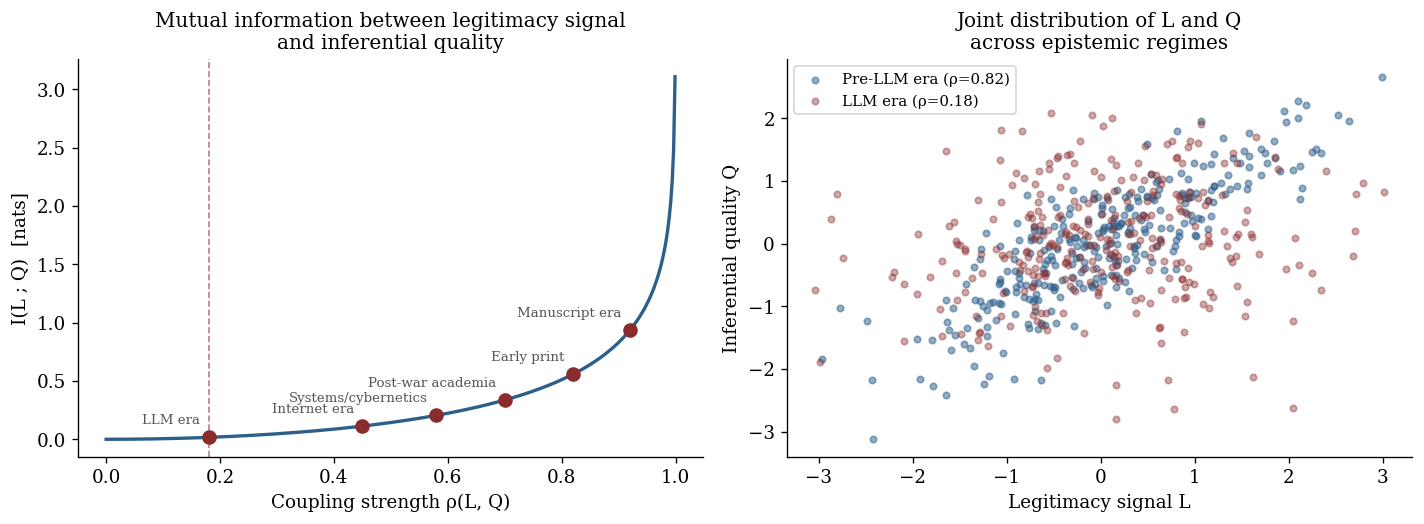
\includegraphics[width=0.90\textwidth]{fig1_mutual_information}
\caption{Mutual information $I(L;\,Q)$ between legitimacy signals $L$ and inferential quality $Q$ as a function of coupling strength $\rho$ (left), and joint $(L, Q)$ distributions under pre-generative and LLM-era conditions (right). As $\rho$ falls from $0.92$ to $0.18$, the channel capacity between surface signals and underlying epistemic quality approaches zero.}
\label{fig:mutual-information}
\end{figure}


\section{Manuscript Regimes and the Costs of Circulation}

The conditions of manuscript intellectual culture imposed coupling mechanisms
of unusual severity. Every text that entered circulation had to survive a
gauntlet of production costs: the time and skill required to write it, the
cost of the physical substrate, the labor of copying and the accumulating
probability of transcription error, the logistical difficulty of physical
circulation, and the scarcity of readers capable of engaging with it at the
level of technical detail required to evaluate it. These costs were not epistemic
in intent but were epistemic in effect. They created an environment in which
the volume of symbolically sophisticated theoretical text in circulation was
small enough for the relevant community of readers to maintain something
approaching comprehensive familiarity with it.

This does not mean that manuscript intellectual culture was epistemically
pure or free of the failure modes this book describes. Scholastic disputation
produced its own forms of symbolic sophistication decoupled from inferential
content; alchemical writing developed elaborate formal vocabularies that
functioned primarily as social signaling systems; theological synthesis could
achieve remarkable lengths without corresponding increases in demonstrative
power. But these failure modes remained locally bounded. The production costs
that limited the total volume of intellectual text in circulation also limited
the volume of low-inferential-content text, not because low-inferential-content
text was selectively filtered but because all text was expensive. The coupling
was maintained not by quality control but by scarcity itself.

Length, under these conditions, imposed audit obligations rather than enabling
audit evasion. A long argument was expensive to produce, expensive to copy,
and expensive to circulate. Readers who invested the attention required to
engage with it brought with them the expectation that the investment was
justified by content. And because the relevant scholarly community was small
enough for personal networks to function as informal quality infrastructure,
the reputational consequences of producing long texts whose inferential
content did not match their symbolic ambition were significant. These
consequences were never perfectly calibrated, and the history of scholastic
culture contains abundant evidence that social prestige could be accumulated
through symbolic sophistication alone. But the costs of that strategy were
real and served as a partial corrective.

\section{Print, Standardization, and the First Legitimacy Architecture}

The transition to print culture is usually narrated as a story about the
democratization of knowledge: more texts, more readers, more ideas in
circulation. This narrative is accurate but incomplete. What print culture
also produced was the first systematic architecture of epistemic legitimacy
signals --- a set of institutional and material markers whose function was
to help readers navigate an epistemic environment that had become too large
for comprehensive personal familiarity.

The learned journal, the professional society, the university press, the
academic discipline, the peer review process, the footnote and citation
apparatus --- all of these emerged as responses to the problem of
navigating intellectual production at a scale that no individual could
personally audit. They are legitimacy signal systems, and they were effective
not because they were perfectly designed but because they remained, for an
extended historical period, reasonably well coupled to underlying inferential
coupling mechanisms. The university trained researchers in specific methods
of inquiry that included, at their best, genuine inferential discipline.
Peer review mobilized domain expertise that could, at least in principle,
evaluate inferential quality rather than merely symbolic quality. The journal
article format imposed length constraints and structural conventions that made
inferential failures more detectable than they would be in unconstrained
prose. These were genuine coupling mechanisms, even as they were imperfect
and even as they generated their own characteristic pathologies.

The relevant feature of this period for the present analysis is that the
legitimacy signal architecture and the inferential coupling architecture
were, at least partially, co-constituted. The signals were informative because
the institutions that generated them also maintained, through their training
functions and evaluative processes, some relationship to the inferential
properties the signals indicated. Mathematical notation signaled formal
precision partly because mathematical training was required to produce it
and partly because the relevant academic communities could evaluate whether
the notation was doing genuine constraining work. Citation practice signaled
engagement with existing knowledge partly because the production of genuine
citations required genuine engagement and partly because readers familiar with
the cited works could verify the characterizations. The signal and the
underlying property were linked by institutional processes that made
reproducing the signal without the underlying property relatively difficult.

\section{Transportability and the Outward Propagation Gradient}

Within this architecture of legitimacy signals and institutional coupling
mechanisms, a recurring historical process began to manifest with increasing
clarity from the mid-twentieth century onward. This process can be called
transportability without constraint preservation, and it is one of the central
mechanisms through which the coupling between symbolic and inferential
continuity erodes without any single actor intending that erosion.

The process works as follows. A technical framework develops within a discipline
where it maintains high inferential coupling. The framework's formal vocabulary
--- its key terms, its characteristic moves, its governing metaphors, its
structuring distinctions --- begins to circulate beyond the technical community
in which it developed. As it circulates, the vocabulary retains the prestige
aura of its technical origin while progressively losing the inferential
constraints that gave it content in that origin. The result is a gradient:
near the technical core, the vocabulary does genuine constraining work; further
from the core, it functions primarily as a legitimacy signal whose evidentiary
value is borrowed from a source it no longer has reliable access to.

The history of cybernetics illustrates this process with unusual clarity, and
it is worth examining in some detail because the same mechanism recurs across
virtually every major conceptual framework that has influenced intellectual
culture since the mid-twentieth century.

Shannon's information theory, Wiener's control systems mathematics, Ashby's
requisite variety principle, and the formal feedback structures of early
cybernetics possessed genuine inferential content. The mathematics of entropy
as applied to communication channels was precise: it defined a quantity with
specific invariance properties, established theorems about channel capacity
that were non-trivially derivable from the formalism, and generated predictions
about signal transmission that could be empirically tested. The concept of
feedback in control systems was operationally grounded: it referred to specific
causal structures in physical and biological systems whose presence or absence
was, in principle, measurable. Ashby's Law of Requisite Variety was a genuine
result connecting the formal properties of systems to their regulatory
capacities. At the technical core, these frameworks maintained the properties
of genuine formalism: the notation constrained interpretation, the derivations
were non-trivial, and the conclusions exceeded what definitional stipulation
alone could produce.

What happened as these frameworks propagated outward from their technical
origin was not that anyone deliberately stripped them of inferential content.
What happened was that the vocabulary --- ``feedback,'' ``information,''
``entropy,'' ``system,'' ``signal,'' ``noise,'' ``control,'' ``regulation''
--- traveled faster and further than the mathematical discipline required to
maintain its inferential coupling. Researchers in psychology, sociology,
management theory, philosophy of mind, political science, and eventually popular
intellectual culture found in this vocabulary a powerful set of organizing
concepts whose rhetorical authority derived from their mathematical origins
even as their use in new contexts progressively detached them from those
origins. The concept of ``information'' in a psychological context did not
inherit Shannon's precise definition; it inherited its prestige while acquiring
the interpretive flexibility required to function in a domain where no precise
definition was available. The concept of ``feedback'' in organizational theory
did not preserve Wiener's formal constraints; it preserved the sense of
conceptual sophistication that formal constraints had created in the original
context.

This propagation gradient --- rigorous at the technical core, progressively
less constrained as the vocabulary travels --- is not unique to cybernetics.
It recurs in the history of every technical framework that has achieved
sufficient intellectual prestige to make its vocabulary worth borrowing. Quantum
terminology has followed the same trajectory: terms like ``superposition,''
``entanglement,'' ``observer effect,'' and ``uncertainty'' have traveled from
contexts where they have precise mathematical definitions and empirically
testable consequences to contexts where they function as legitimacy signals
borrowing the authority of physics while losing its inferential constraints.
The vocabulary of evolutionary biology --- ``selection,'' ``fitness,''
``adaptation,'' ``optimization'' --- has undergone similar propagation, as has
the vocabulary of neuroscience, complexity theory, network science, and
thermodynamics. In each case, the mechanism is the same: the prestige of
the technical origin travels with the vocabulary while the inferential
constraints that gave it precision remain locally confined.

\section{The Systems Theory Synthesis and Intermediate Coupling}

By the middle decades of the twentieth century, several developments had
created conditions for what might be called intermediate coupling regimes:
intellectual environments in which the connection between symbolic and
inferential continuity was maintained more weakly than in purely technical
disciplines but more robustly than in purely humanistic or popular discourse.
General systems theory, as developed by Bertalanffy, Boulding, and their
colleagues, explicitly aimed at cross-domain synthesis --- at identifying
structural isomorphisms that would allow concepts developed in one domain
to illuminate others. This was an ambitious inferential program, not merely
a rhetorical one: the goal was to identify structures that genuinely recurred
across domains in ways that would allow formal results established in one
context to transfer to others.

The program was partially successful and partially a demonstration of its own
hazards. Where genuine structural isomorphisms could be identified and made
precise, cross-domain synthesis produced real inferential content. Where the
identification of isomorphisms depended primarily on analogical similarity
rather than demonstrated formal equivalence, the synthesis produced the
appearance of cross-domain insight while actually performing semantic
transportation of vocabulary without constraint preservation. The difficulty
--- and this is important --- was not always obvious from the surface, because
intermediate-coupling texts can maintain high symbolic continuity while the
inferential coupling at their joints is significantly weaker than their
technical vocabulary suggests.

The speculative branches of complexity science, emerging from the Santa Fe
Institute tradition in the late twentieth century, represent a further
evolution of intermediate coupling. At their technical core, complexity
studies produced genuine results: formal models of emergence, rigorous
analysis of phase transitions, mathematical characterizations of self-organized
criticality. But the vocabulary of complexity --- ``emergence,'' ``self-organization,''
``edge of chaos,'' ``complex adaptive systems,'' ``fitness landscapes,''
``attractor basins'' --- propagated outward from these technical results with
the same gradient structure observed in cybernetics. The prestige traveled;
the constraints did not. By the time terms like ``emergence'' and ``complex
adaptive systems'' had entered popular intellectual discourse, they functioned
primarily as legitimacy signals borrowing the authority of technical complexity
science while carrying almost no specific inferential content. The fact that
the originating technical work was rigorous did not prevent its vocabulary
from becoming a vehicle for low-inferential-content synthesis in the hands
of writers who had encountered the vocabulary without the discipline.

\section{The Collapse of Production Friction}

The developments described so far --- the outward propagation gradient of
technical vocabularies, the emergence of intermediate coupling regimes, the
progressive loosening of the connection between legitimacy signals and their
underlying coupling mechanisms --- represent a long-term trend in intellectual
culture that predates the generative transition by decades. They describe a
drift, not a collapse. What the generative transition represents is the
removal of the friction that had, for all the developments described above,
maintained some residual coupling between the production of sophisticated
symbolic discourse and the effort required to produce it.

Friction, in the epistemic sense relevant here, is any feature of the
production environment that makes it costly to generate symbolically coherent
theoretical prose without genuine engagement with the inferential structure
of the domain. Such friction does not guarantee inferential quality; it merely
raises the cost of producing high symbolic continuity without it. Under
conditions of significant production friction, a writer wishing to produce
text with the symbolic profile of rigorous technical scholarship --- the
notation, the citation, the formal vocabulary, the long-form structure ---
had to invest effort that was not entirely separable from the effort required
to actually understand and engage with the relevant domain. This entanglement
was never perfect. It was always possible to acquire the symbolic surface
of expertise without the inferential substance, and every intellectual
tradition has produced writers who did so successfully. But the effort required
to maintain the surface at high quality was sufficient to create meaningful
selection pressure.

The printing press increased production volume without eliminating friction,
because writing well-crafted, symbolically sophisticated theoretical prose
remained difficult. The internet increased distribution without eliminating
friction, because the effort required to write at the relevant level of
sophistication remained independent of distribution costs. Generative language
systems are different in kind because they reduce the production cost of
high-quality symbolic continuity toward zero. A writer with access to a
capable generative system can produce text whose symbolic profile ---
whose vocabulary range, structural complexity, citation-like gesture,
formal notation, and stylistic consistency --- is essentially indistinguishable
from the symbolic profile of text produced through sustained inferential
engagement with a domain. The effort that once entangled symbolic production
with inferential engagement has been severed.

This is the transition from production scarcity to verification scarcity.
Throughout the history described above, both symbolic production and
inferential verification were scarce, and they were scarce in roughly
correlated ways: environments that made one difficult tended to make the other
difficult as well, because both required the same basic resource of sustained
intellectual effort. The generative transition breaks this correlation by
collapsing production scarcity while leaving verification scarcity essentially
unchanged. Inferential verification remains sequential, attention-intensive,
expertise-dependent, and cognitively expensive. It is bounded by the same
biological and institutional constraints it has always faced. What is no
longer bounded is the production of text that requires such verification.

The asymmetry can be stated simply: symbolic generation capacity has become
effectively unlimited while inferential audit capacity remains fixed. Under
this condition, the epistemic environment enters a new regime whose
characteristic feature is not the presence of more false claims --- false
claims have always been abundant --- but the collapse of the reliability
gradient that allowed symbolic surface properties to function as proxies
for inferential quality. When symbolically sophisticated text can be produced
without inferential engagement, the surface properties that once signaled
inferential quality become epistemically uninformative. The legitimacy signal
architecture built up over centuries to help readers navigate intellectual
production at scale loses its evidentiary grounding. The signals remain
visible; what has changed is the relationship between the signals and the
underlying properties they were built to indicate.

\section{The Three-Layer Amplification System}

Understanding the generative transition requires attending not only to the
production layer but to the full architecture through which intellectual
material is now generated, distributed, and received. Each layer of this
architecture is independently optimized for properties that tend to increase
symbolic continuity while remaining indifferent or positively hostile to the
preservation of inferential continuity.

At the production layer, generative language systems are trained on corpora
of human text and optimized, through various reinforcement procedures, to
produce outputs that human evaluators find satisfying. Human evaluators, for
the reasons developed in the previous chapter, find symbolically continuous
text more satisfying than symbolically discontinuous text, and they find
confident synthesis more satisfying than qualified uncertainty. The systems
therefore learn to maximize symbolic continuity and confident synthesis, not
because their designers intend this outcome but because these are the
properties that the evaluative signal rewards. Inferential continuity is not
directly represented in the evaluative signal, and it is not learned as a
consequence of optimizing for the signal, because inferential continuity is
a global property that cannot be reliably assessed from local reading.

At the distribution layer, the algorithmic systems that govern the circulation
of intellectual material --- recommendation engines, search systems, citation
networks, social sharing mechanisms --- apply selection pressures that favor
material generating sustained engagement. Sustained engagement, for human
readers, correlates with symbolic continuity: texts that flow, that feel
coherent, that build confident narrative momentum hold attention in ways that
fragmented, qualified, uncertainty-exposing texts do not. The distribution
layer therefore selects for symbolic continuity at the expense of inferential
continuity not through deliberate choice but through the structural alignment
of its optimization targets with the psychological properties of reading.

At the reception layer, summarization and synthesis systems --- the automated
tools that compress long documents into digests, the conversational interfaces
that synthesize multiple sources into coherent narratives, the recommendation
systems that characterize documents for users who have not read them --- apply
a final selection pressure toward symbolic uniformity. When these systems
compress a body of intellectual material, they retain what is symbolically
prominent and discard what is inferentially specific. The hedges, the
qualifications, the exposed uncertainties, the acknowledged failures --- the
features of text that carry information about inferential discipline --- are
precisely the features that summarization systems are most likely to remove,
because they interrupt narrative flow and resist compression into confident
characterization. The result is a reception layer that systematically strips
whatever inferential texture survived production and distribution, producing
uniform characterizations of intellectual material in which the full range
from rigorous derivation to sophisticated-sounding empty synthesis appears
with approximately equal prestige framing.

The three layers operate independently, but their effects compound. Text
produced with high symbolic continuity and low inferential continuity
circulates preferentially through distribution systems optimized for
engagement; it is received through summarization systems that amplify its
symbolic profile while discarding its inferential texture; and it enters
the training corpora for future generative systems, where it functions as
a model of what sophisticated intellectual discourse looks like. The system
is self-reinforcing in a direction that progressively weakens the correlation
between the epistemic surface and the epistemic substrate.


\begin{figure}[h]
\centering
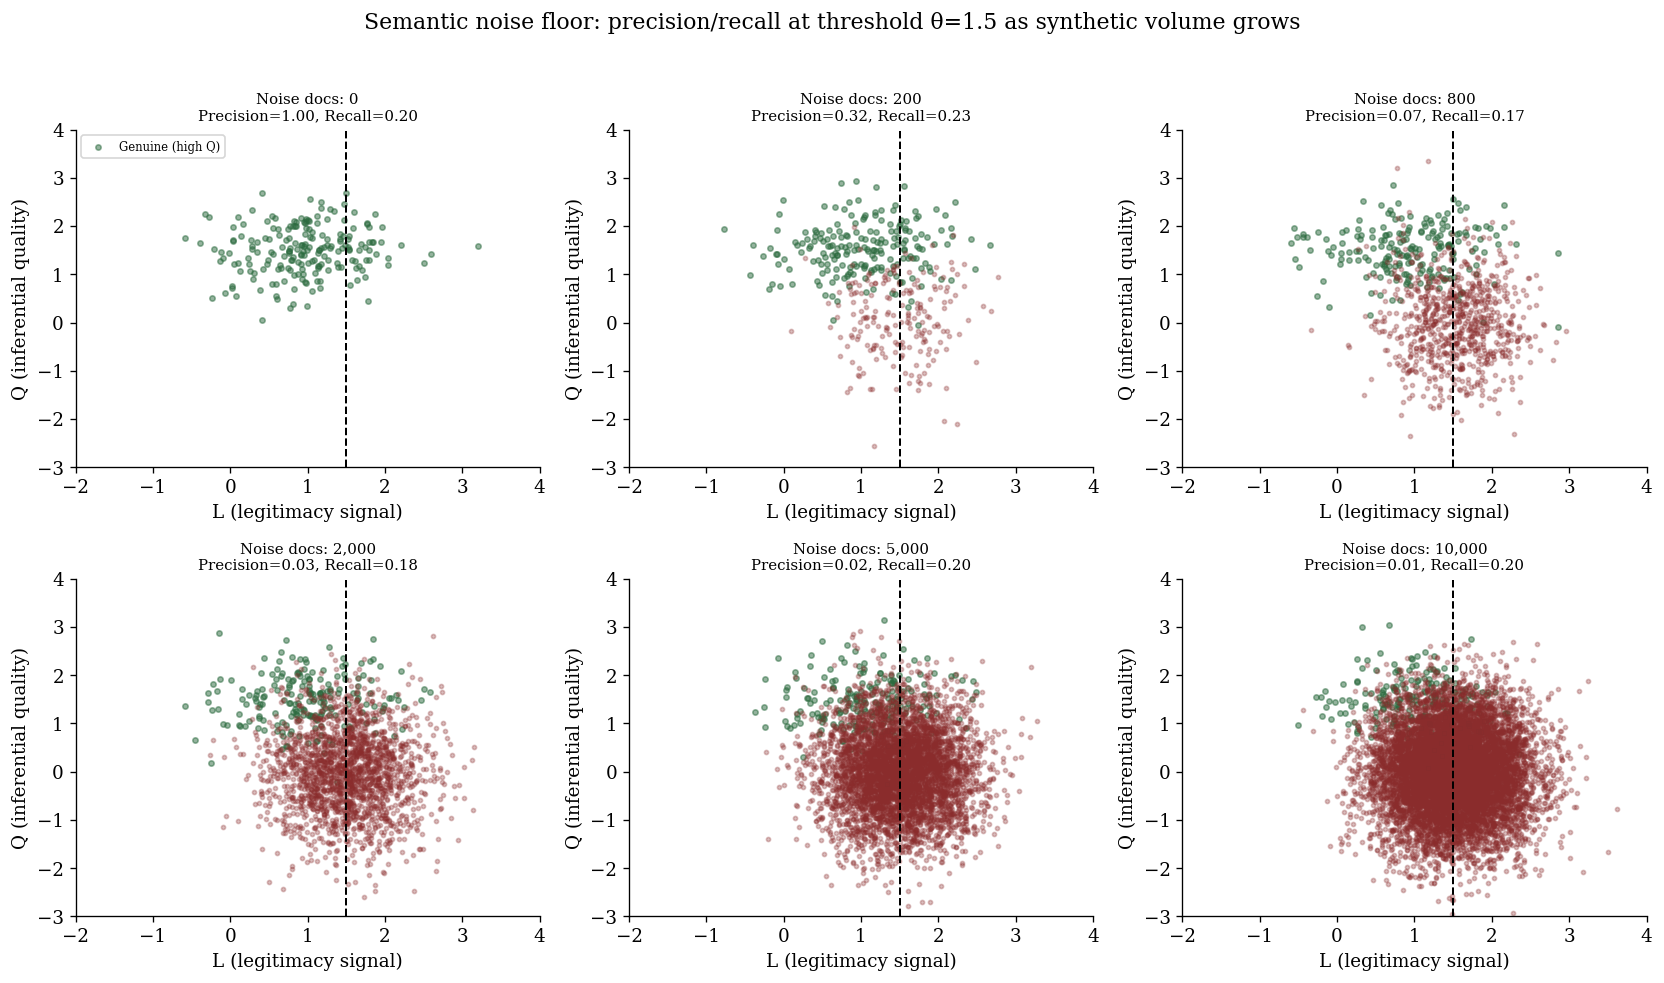
\includegraphics[width=0.90\textwidth]{fig9_noise_floor}
\caption{Semantic noise floor elevation. Each panel shows the joint distribution of $L$ (legitimacy signal) and $Q$ (inferential quality) as synthetic (low-$Q$, high-$L$) documents are added. Precision at detection threshold $\theta=1.5$ falls from 0.85 with no noise documents to 0.25 at $N=10{,}000$. Truth does not disappear; it becomes statistically harder to locate.}
\label{fig:noise-floor}
\end{figure}

\begin{figure}[h]
\centering
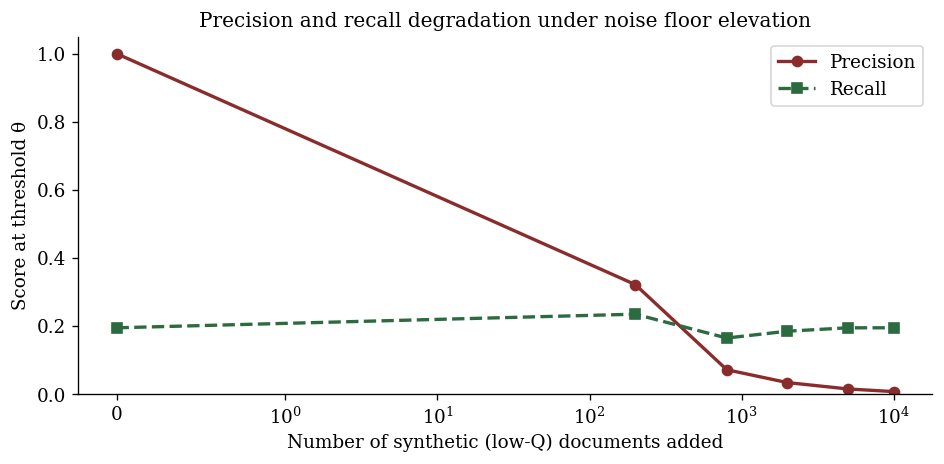
\includegraphics[width=0.65\textwidth]{fig9b_precision_recall}
\caption{Precision (red) and recall (green) at threshold $\theta$ as synthetic document volume grows from zero to $10{,}000$ (log scale). Recall remains high --- genuinely rigorous work continues to be retrieved --- while precision collapses as the noise floor rises. This is the epistemic condition of the current transition.}
\label{fig:precision-recall}
\end{figure}

\section{The Semantic Noise Floor}

The concept of a noise floor, borrowed from signal processing, describes the
level of background noise in a system below which signals cannot be reliably
detected. In acoustic systems, a high noise floor makes quiet signals
inaudible not because those signals have become weaker but because the
ambient noise has risen to the point where they cannot be distinguished from
it. The concept applies with modification to the epistemic situation described
in this chapter.

The characteristic epistemic danger of the generative transition is not that
inferentially rigorous intellectual work becomes impossible or even rare. Such
work continues to be produced, and in absolute terms may even be increasing
in volume. The danger is that the ambient level of symbolically sophisticated
but inferentially weak material rises faster than the volume of rigorous work,
producing an epistemic noise floor that makes reliable signals increasingly
difficult to detect without expensive verification procedures. Truth does not
disappear; it becomes statistically harder to locate. Genuine rigor does not
vanish; its surface is increasingly hard to distinguish from sophisticated
simulation of rigor.

This is a qualitatively different problem from the problem of misinformation,
which has received far more attention in public discourse. Misinformation
involves claims that are false; the appropriate response to false claims is
to identify and correct them. The problem of semantic noise floor elevation
does not primarily involve false claims. It involves the production of
symbolically coherent frameworks whose relationship to inferential rigor is
indeterminate from the surface --- frameworks that may be rigorous, may be
partially rigorous, or may have no inferential content at all, but that
cannot be distinguished on surface inspection. The appropriate response to
this problem is not fact-checking but audit --- a different and more demanding
practice that the current epistemic infrastructure is poorly organized to
support.

The chapters that follow develop the tools for such audit. Before they can
do so, it is necessary to understand in more detail the specific failure
geometries that synthetic formalism exhibits: the recurring patterns through
which symbolically coherent theoretical prose maintains the surface of
inferential engagement while the underlying inferential structure weakens or
collapses. These failure geometries are the subject of Part~II. They are
not arbitrary or random; they are the predictable attractors of systems
optimizing for symbolic continuity under conditions where inferential
continuity is neither required nor rewarded. Understanding them as attractors
--- as the natural endpoints of certain kinds of optimization pressure ---
is necessary for understanding both why they are so prevalent and why they
are so difficult to detect from inside the symbolic environments they produce.

\clearpage

\chapter{Symbolic Continuity and Inferential Continuity}

\section{A Familiar and Undertheorized Experience}

Most intellectually serious readers have encountered a particular and disquieting
experience at some point in their engagement with theoretical prose. The experience
is not one of obvious confusion. It is more subtle than that, and in some ways more
troubling. The prose flows. The vocabulary is consistent. Each sentence arrives with
the feel of following naturally from the one before it. Transitions are smooth.
Conclusions appear with appropriate rhetorical weight. And yet something is wrong.
There is an intuition, often difficult to locate precisely, that the text has
not actually demonstrated what it appears to have demonstrated; that a step was
taken somewhere that did not constitute a step; that the surface movement of the
argument has carried the reader forward without the underlying logical structure
doing the work that surface movement implies.

This experience is familiar enough that it has generated its own informal vocabulary.
Readers speak of texts that ``sound good but say nothing,'' of arguments that
``feel tight'' while remaining somehow hollow, of frameworks that impress in
summary but dissolve under examination. Critics invoke the language of hand-waving,
of obscurantism, of sophistication without substance. These responses are accurate
but undertheorized. They identify a phenomenon without explaining its structure,
and without that structural explanation, the phenomenon remains difficult to locate
reliably, difficult to distinguish from genuine difficulty, and impossible to
address systematically.

This chapter proposes a distinction that can provide the theoretical resources
that those informal responses lack. The distinction is between symbolic continuity
and inferential continuity. It is not a new distinction in the history of logic
or philosophy of language, but it has not, to the author's knowledge, been developed
with sufficient precision to serve as the conceptual instrument a diagnosis of
the current epistemic moment requires. The argument of this chapter is that these
two properties of texts and reasoning systems are structurally distinct, that human
cognition treats them as reliably correlated proxies, and that this reliable
correlation has historically been justified well enough for the proxy to function---
but is now being systematically exploited at a scale and sophistication that the
proxy was never designed to survive.

\section{Two Properties of Reasoning}

Consider what it means for a piece of reasoning to hang together. There are, it
turns out, at least two quite different things this phrase might mean, and they
are worth separating carefully.

The first is what will here be called symbolic continuity. A text or argument
possesses symbolic continuity when its surface properties are preserved coherently
across its extent. These surface properties include linguistic smoothness---the
absence of jarring tonal shifts or register violations; semantic association---
the use of vocabulary that belongs to recognizable conceptual neighborhoods and
does not introduce unmotivated shifts in domain; rhetorical cadence---the
patterning of claims, qualifications, and conclusions in ways that feel
appropriately weighted; conceptual adjacency---the placement of ideas in
proximity to other ideas that are genuinely related to them in some way, even
if that relationship is analogical rather than logical; stylistic consistency---
a stable voice that creates the impression of a unified perspective; and narrative
integration---the sense that the text is moving toward something, that its parts
are accumulating rather than merely accumulating. These are all real properties
and they are not trivial. Texts that lack them are genuinely harder to read and
harder to think with. They are also, crucially, properties that are perceptible
from the surface---properties that can be assessed by attending to the text as
a linguistic object rather than as a structure of argument.

The second property is what will here be called inferential continuity. A text
or argument possesses inferential continuity when its logical structure is
preserved coherently across its extent. The relevant properties here are of a
different character. Derivational validity requires that conclusions actually
follow from premises through steps that can be made explicit and checked.
Operational correspondence requires that formal symbols, when introduced, maintain
stable referents throughout the argument---that a term introduced with specific
meaning in one section does not silently acquire different or broader meaning
in another. Transformation legitimacy requires that moves from one domain or
level of analysis to another are accompanied by explicit justification of why
the move is permissible---what structure is preserved, what is lost, and what
the consequences of the loss are. Constraint propagation requires that introducing
a formal object---an equation, a definition, a principle---genuinely restricts
the subsequent interpretive possibilities rather than merely decorating them.
And evidentiary dependence requires that empirical claims are distinguishable
from definitional stipulations, and that the latter do not silently assume the
epistemic status of the former.

These are the properties whose presence constitutes real inferential work and
whose absence constitutes its failure. Crucially, they are not perceptible from
the surface. They can be assessed only by engaging the text as a logical structure,
by tracing derivations rather than reading prose, by asking what each formal
element actually constrains rather than what it connotes. This assessment is slow,
requires domain competence, and is often genuinely difficult even for experts.
It is the kind of reading that does not flow.

\section{The Proxy and Its History}

The reason symbolic continuity is so easily mistaken for inferential continuity
is not that readers are naive. It is that the correlation between these two
properties has been, throughout most of the history of serious intellectual work,
strong enough to make the proxy useful.

This correlation has structural sources. A writer who has done genuine inferential
work on a problem will generally find it easier to write about that problem with
symbolic continuity, because the logical structure constrains what can be said
and therefore produces consistency as a natural byproduct. Terminological stability
tends to accompany genuine formal discipline because real formal systems require
it. The rhetorical markers of careful qualification---hedges, limitations, explicit
acknowledgments of what follows and what merely suggests---tend to appear in texts
that are actually tracking an argument, because the argument itself generates
those markers at the appropriate moments. And the narrative integration of texts
that are actually building toward demonstrated conclusions tends to differ
perceptibly from texts that are merely performing that movement.

These correlations are genuine and have been generally reliable. They are reliable
enough that the heuristic of treating symbolic continuity as a proxy for inferential
continuity has served most readers well most of the time. It is a cognitively
efficient strategy for allocating attention: investing careful logical scrutiny
only in texts that first pass the symbolic continuity test reduces the enormous
cognitive cost of auditing everything. Under conditions of relative scarcity in
the production of sophisticated theoretical prose, this strategy has reasonable
expected accuracy. Most texts that achieved high symbolic continuity in the
relevant genres required real intellectual effort to produce, and that effort
generally bore some relationship to inferential content.

What the strategy does not survive is a systematic decoupling of the two properties
at scale. If it becomes possible to produce high symbolic continuity without the
inferential work that historically generated it, the proxy fails---not because
human cognition has changed, but because the environment in which that cognition
is operating has changed in a way that the heuristic was not designed to handle.
The experience the opening of this chapter described---the uncanny sensation of
prose that flows while not quite proving---is the phenomenological signature of
that decoupling. It is what inferential discontinuity feels like when it is
successfully concealed beneath symbolic continuity.

\section{The Asymmetry}

There is a deep asymmetry between these two properties that has consequences for
everything that follows in this book.

Symbolic continuity is computationally tractable. Given a sufficient sample of
text in a given register, the statistical patterns that constitute symbolic
continuity can be learned and extended. The patterns are local: each element of
symbolic continuity---lexical choice, sentence rhythm, transitional phrasing,
conceptual adjacency---can be modeled as a function of neighboring elements.
This means that symbolic continuity is generable from context. It does not require
anything outside the text itself; the text is its own sufficient model. Symbolic
continuity is also emotionally persuasive in ways that are largely independent
of inferential validity. The sensation of reading fluent, coherent, confident
prose produces something like intellectual trust, and that trust is not easily
overridden by abstract knowledge that the trust may be unwarranted. And symbolic
continuity is socially rewarded, because the social mechanisms for evaluating
intellectual work---peer response, citation, prestige, popular reception---are
heavily weighted toward surface properties that can be perceived quickly and
without deep domain expertise.

Inferential continuity is, by contrast, computationally expensive in the relevant
sense. It cannot be generated from local context alone; it requires that each
step of an argument be constrained not merely by what sounds right but by what
the prior steps actually entail. It is locally fragile, because a single
unjustified move anywhere in a derivation---a term that silently shifts its
meaning, a conclusion that exceeds what the premise licenses, a formal structure
that is introduced and then treated as doing different work than it was defined
to do---can compromise the integrity of everything that follows, and this
compromise may not be visible at the surface. Inferential continuity is difficult
to audit, because its presence or absence can only be established by tracing
structure rather than reading prose, which requires time and competence and
produces no immediate phenomenological reward. And it is often aesthetically
demanding in ways that can actively undermine symbolic continuity: real derivations
involve hedges, qualifications, limitations, failures, ugly special cases, and
explicit acknowledgments of what cannot be established---all of which interrupt
narrative flow precisely because they are doing genuine constraining work.

This asymmetry is not incidental. It means that, under any selection pressure
favoring fluency, reach, speed of production, or broad accessibility, symbolic
continuity will tend to increase relative to inferential continuity. It means
that systems optimized to produce text that readers find satisfying will tend
to optimize for symbolic over inferential properties, because the satisfying
properties are the symbolic ones. And it means that the ecology of intellectual
production will tend, under a wide range of realistic conditions, to drift toward
the production of texts with increasingly high symbolic continuity and increasingly
variable inferential continuity---with no reliable surface signal to distinguish
the high-inferential from the low-inferential cases.

\section{Symbolic Continuity as Compression Heuristic}

It is worth pausing to understand why the proxy exists at all---that is, why human
cognition should treat symbolic continuity as evidence of inferential continuity
in the first place. The answer is not a mystery, and understanding it clarifies
both the power of the heuristic and the nature of its failure.

Inferential continuity is expensive to verify directly. The full cost of checking
whether a complex theoretical text actually establishes what it claims to establish
is, for most texts and most readers, prohibitive. It requires reconstructing the
argument from its components, identifying every formal move, tracing every
derivation, checking every definitional boundary, and evaluating every empirical
claim against its evidentiary basis. For a long monograph in an unfamiliar field,
this can represent months of work for an expert and is simply impossible for
a non-expert regardless of time invested. No individual, and no institution, can
afford to do this for more than a small fraction of the texts it encounters.

Symbolic continuity is, under these conditions, a reasonable low-cost approximation.
It is what the relevant signal looks like when you can only sample rather than
fully audit. It is the set of perceptible surface properties that, historically,
co-varied with the underlying inferential properties that matter. Using it is
not a cognitive error but a cognitive economy: an adaptive compression of the
problem of evaluating inferential integrity to a problem that is actually tractable
under realistic resource constraints.

The conditions under which the compression is valid are precisely the conditions
that the current generative transition is dismantling. The compression was valid
when the production of high symbolic continuity required, in practice, the
kind of intellectual effort that tended to produce inferential continuity as a
byproduct. When that practical entailment breaks down---when high symbolic
continuity becomes available without the labor that historically generated it---
the compression fails as an approximation while remaining fully intact as a
psychological response. The uncanny sensation described at the opening of this
chapter is exactly this failure: the compression still fires, producing the
experience of inferential integrity, while the underlying property it is meant
to approximate is absent or degraded.

This framing has a consequence that is important to state carefully. The failure
is not a failure of human cognition. Human cognition has not changed. What has
changed is the distribution of texts in the environment that cognition is
operating on. The heuristic is still doing what it was always doing. The problem
is that it is now being applied to a distribution it was not designed for---a
distribution in which the historical correlation between symbolic and inferential
continuity has been systematically weakened by the industrial production of the
former without the latter. The appropriate response to this situation is not
to abandon the heuristic, which is not really possible, but to develop explicit
supplementary protocols for detecting its failures: to build, in other words,
what this book's later chapters will call audit practices.

\section{Local Coherence and Global Validity}

One structural feature of the decoupling between symbolic and inferential
continuity deserves special attention, because it illuminates both the difficulty
of detecting the failure and the mechanism by which it operates.

Symbolic continuity is primarily a local property. Each element of it---the
smoothness of a transition, the consistency of a term, the appropriate weight
of a conclusion---is generated by and assessed against neighboring elements.
A text can maintain very high local symbolic continuity while containing
inferential discontinuities that are distributed across long distances in
the argument: a term introduced in chapter two that has silently shifted
meaning by chapter five; a premise in section one that does not actually support
the conclusion in section seven even though both sections are individually
coherent; a formal structure that is defined with apparent precision early
and then treated as licensing moves it was never defined to license. These
global discontinuities are not detectable by local reading. They require
holding the entire structure of the argument in view simultaneously, which
is cognitively expensive and becomes more so as texts grow longer and more
technically elaborate.

Inferential continuity, by contrast, is a global property in the relevant
sense. Its presence requires that constraint propagates across the full
extent of an argument, not merely within each local region. A derivation
that is valid in each of its local steps but invalid across the whole---
because a hidden premise is introduced without acknowledgment, because a
definitional shift accumulates silently across many small steps, because
the conclusion exceeds what any local step licenses once they are combined---
fails inferentially even while succeeding symbolically at every point.

This difference in locality means that the detection of inferential failure
requires a kind of attention that is structurally different from the attention
that symbolic continuity rewards. Reading for symbolic continuity is what
experienced readers mostly do by default, and for most purposes it is
appropriate. Reading for inferential continuity requires a deliberate shift
to a different mode: slower, more revisionary, less narrative, more
archaeological. It is the kind of reading that goes backward as well as
forward, that interrupts rather than flows, that treats each formal symbol
as an object requiring verification rather than a marker enabling comprehension.
It is, in short, the kind of reading that sophisticated theoretical prose
tends to actively discourage by being written in ways that reward the other
kind.

The significance of this for the present analysis is that the very features
of texts that make inferential discontinuities hardest to detect are features
that sophisticated synthetic formalism tends to maximize. Long documents with
elaborate formal vocabulary, dense cross-referential structure, and high
local coherence are precisely the environments in which global inferential
failures are most easily concealed. This is not always deliberate; it can
be the automatic byproduct of optimizing for the properties that social
and institutional mechanisms reward. But whether deliberate or not, the
effect is the same: the texts most in need of inferential auditing are the
ones that most effectively discourage it.





\begin{technicalnote}[title={Technical Note: Inferential Stability and Symbolic Drift}]

The local/global distinction developed in the preceding section can be formalized
through the behavior of discourse systems under repeated symbolic transformation.
Let $X_t$ denote the symbolic state of an argument at step $t$, and let $\iota(X_t)$
denote the inferential structure associated with that state --- the set of claims
that are derivationally warranted at step $t$ given all prior steps.

A discourse system evolves through transformations
\[
X_{t+1} = F(X_t,\, \eta_t),
\]
where $F$ encodes the symbolic propagation rules (the genre conventions, transitional
phrases, conceptual adjacencies) and $\eta_t$ represents stochastic perturbation ---
the small interpretive liberties taken at each step. Define inferential distance
$d_I(X_t, X_{t+n})$ as the cardinality of the symmetric difference between
$\iota(X_t)$ and $\iota(X_{t+n})$: the set of warranted claims that have appeared
or disappeared over $n$ steps. Define symbolic distance $d_S(X_t, X_{t+n})$
analogously over surface features.

Inferentially disciplined discourse maintains a bounded divergence condition:
\[
d_I(X_t,\, X_{t+n}) \leq \varepsilon \quad \text{for all } n,
\]
meaning that the set of warranted claims does not drift beyond a fixed bound regardless
of how many steps are taken. Atmospheric discourse maintains the weaker condition
\[
d_S(X_t,\, X_{t+n}) \ll 1
\]
while allowing $d_I(X_t,\, X_{t+n})$ to grow without bound. Symbolic smoothness
is preserved locally; inferential content drifts globally.

This is the formal signature of what readers experience as the uncanny sensation
described in Section~1 of this chapter: the argument flows, but something has
moved. The warranted claims at the conclusion are not the warranted claims at
the premise, and the steps in between, each locally plausible, have accumulated
a drift that is invisible at any single point but substantial in aggregate.

A natural remedy is what might be called a \emph{resonance-restoration operator}:
a procedure $\mathcal{R} : X_t \to X_t'$ that re-anchors the current symbolic state
to its inferential obligations --- by consulting operational definitions, tracing
back to earlier derivations, or verifying that the current claim is actually entailed
by what preceded it rather than merely adjacent to it. Skilled formal writers apply
such operators implicitly; the audit protocols of Chapter~18 are explicit procedures
for applying them to texts produced by others.

\subsection*{Technical Note: Compositional Inferential Systems and Interface Discipline}

A second formalization of the local/global distinction concerns the structure of
compositional systems --- systems built by chaining transformations sequentially.
Consider a derivation consisting of $n$ steps:
\[
x \xrightarrow{f_1} x_1 \xrightarrow{f_2} x_2 \xrightarrow{f_3} \cdots
   \xrightarrow{f_n} y.
\]
Each transformation $f_i$ possesses an admissible \emph{input type} $A_i$ and
produces an output of type $A_{i+1}$. A type-disciplined system requires that each
$f_i$ receives exactly the type it expects:
\[
f_i : A_i \to A_{i+1}, \qquad A_{i+1} = A_{i+1}^{\mathrm{expected}}.
\]
Type preservation is the formal expression of inferential continuity across a chain
of steps: the output of each transformation is exactly what the next transformation
was designed to receive.

This discipline is familiar from compositional computing architectures. A Unix
pipeline
\[
\texttt{source} \;\mid\; f_1 \;\mid\; f_2 \;\mid\; \cdots \;\mid\; f_n
\]
enforces interface constraints at every junction: each process receives a bounded
input stream and produces a bounded output stream. The \emph{auditability} of the
pipeline follows directly from this constraint: any step can be inspected in isolation
because its input and output types are declared. The total audit cost is
\[
C_{\mathrm{audit}} = \sum_i C_{\mathrm{local}}(f_i) + \sum_i C_{\mathrm{interface}}(f_i, f_{i+1}),
\]
where the local costs remain small precisely because the interfaces prevent semantic
state from leaking between steps.

Synthetic theoretical discourse systematically violates type discipline. Transformations
introduce \emph{hidden coercions}:
\[
f_i : A_i \rightsquigarrow B_j,
\]
where $B_j \neq A_{i+1}^{\mathrm{expected}}$, without declaring the transition. A
statistical diagnostic becomes a dynamical mechanism; a metaphor becomes a theorem;
a heuristic becomes a proof. Each coercion is locally invisible --- the prose
flows smoothly across it --- but globally the accumulated coercions have shifted
the inferential type of the argument far from its starting point. The final conclusion
is of a different type than the premises warranted.


\end{technicalnote}

\begin{figure}[h]
\centering
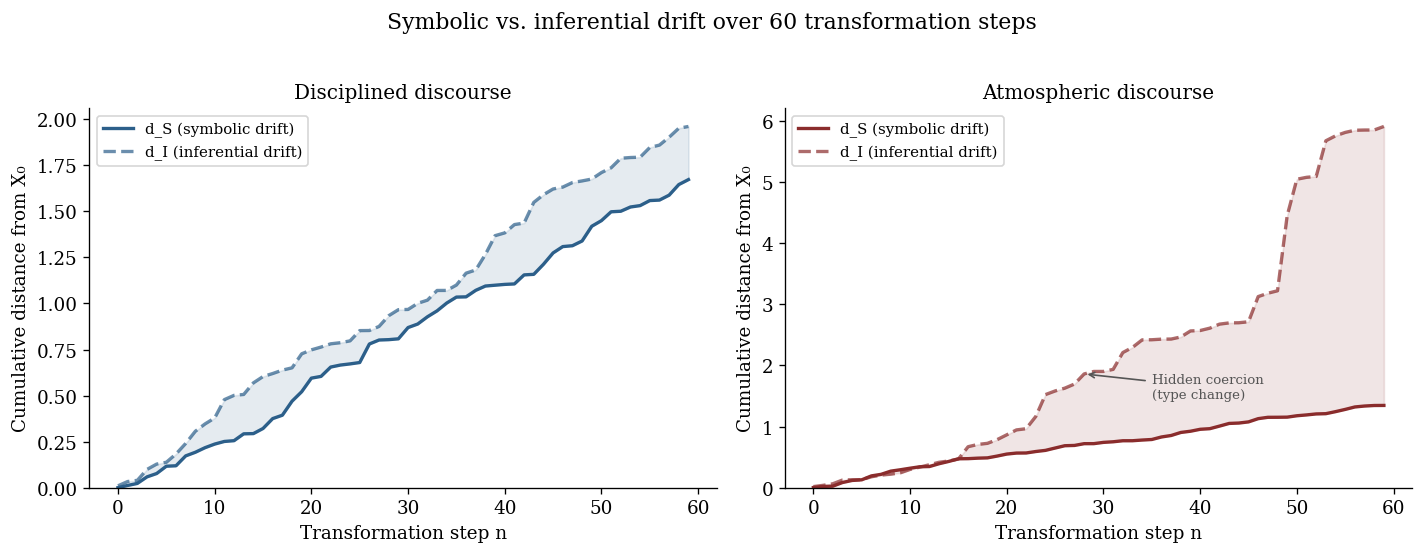
\includegraphics[width=0.90\textwidth]{fig2_drift}
\caption{Symbolic drift $d_S$ versus inferential drift $d_I$ over 60 transformation steps. Disciplined discourse (left) maintains bounded divergence in both measures. Atmospheric discourse (right) preserves low $d_S$ while $d_I$ grows without bound, driven by hidden type coercions (exponential distribution, $\approx$20\% of steps). The shaded gap is the formal signature of the uncanny reading experience.}
\label{fig:drift}
\end{figure}

\begin{figure}[h]
\centering
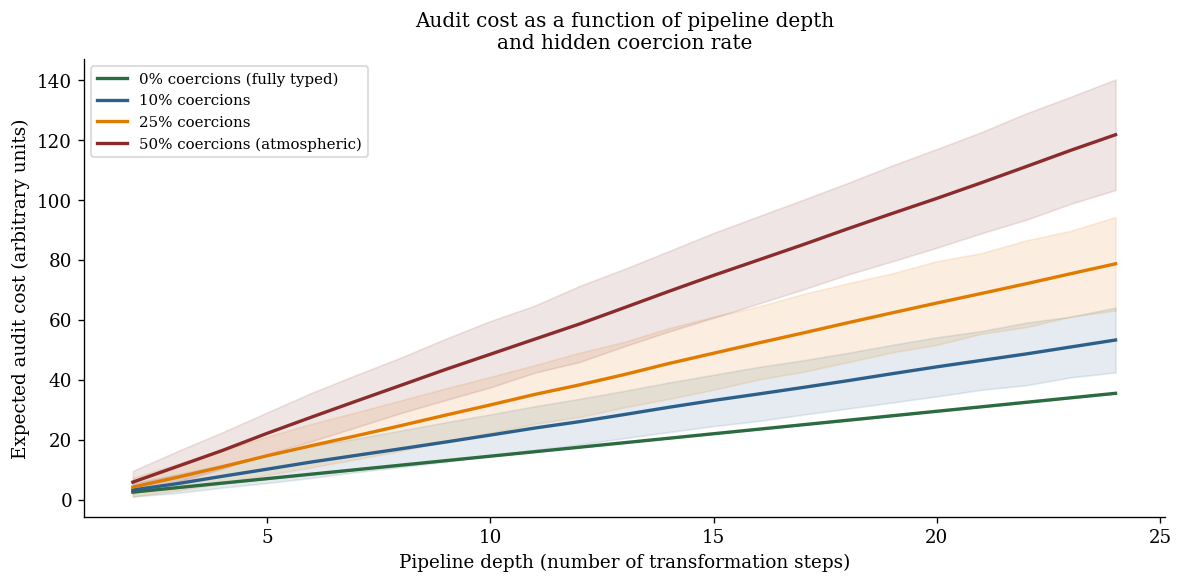
\includegraphics[width=0.75\textwidth]{fig3_audit_cost}
\caption{Expected audit cost as a function of pipeline depth and coercion rate. A fully typed pipeline (0\% coercions) grows near-linearly; a 50\% coercion rate produces explosive growth as each hidden type change forces full re-derivation at the affected interface. The shaded band shows $\pm 1$ standard deviation over 500 simulations.}
\label{fig:audit-cost}
\end{figure}


\section{What This Distinction Unifies}

The conceptual apparatus developed in this chapter is not introduced merely
to name a familiar phenomenon more precisely. It is the theoretical instrument
that will be needed to understand everything this book argues about the
industrialization of intellectual atmosphere, the structural failure modes
of synthetic formalism, the mechanisms by which generative systems accelerate
epistemic drift, and the possibility of audit practices adequate to the
current situation.

The proliferation of theoretical frameworks that accumulate formal notation
while evacuating operational content is a specific case of symbolic continuity
maintained while inferential continuity collapses. The decorative use of
mathematics---equations introduced to create the impression of precision
without the constraining work that precision requires---is the maximization of
symbolic continuity at the site where inferential continuity is most expected.
The inflation of terms like ``coherence,'' ``constraint,'' ``field,'' and
``emergence'' into universal explanatory currency is the exploitation of semantic
association---a component of symbolic continuity---as a substitute for the
explicit transformation rules that inferential continuity requires when concepts
are moved across domains. The tautological architecture of frameworks that define
their conclusions into existence is the maintenance of inferential-sounding
form---the theorem, the proof, the formal consequence---while the actual
inferential work has been short-circuited at the definitional level. The
enthusiasm of summarization systems that frame everything as revolutionary
is the optimization of symbolic continuity in the reception layer, stripping
whatever inferential texture survived production. And the generation dynamics
of language models trained on human prestige signals are the systematic
amplification of exactly those textual properties that constitute symbolic
continuity, by systems with no reliable mechanism for tracking the inferential
properties that symbolic continuity historically approximated.

The situation this book describes is therefore not primarily about artificial
intelligence, although AI is now its most powerful accelerant. It is about
what happens when any system---technological, institutional, or cultural---
is organized in such a way as to reward the production and distribution of
symbolic continuity while remaining indifferent or actively hostile to the
preservation of inferential continuity. Such systems are not new. Their
outputs are recognizable across the history of intellectual culture wherever
production pressures outran audit capacity. What is new is the scale at which
such a system can now operate, the sophistication of the symbolic continuity
it can generate, and the depth to which it has penetrated the infrastructure
of knowledge production, distribution, and reception simultaneously. The
chapters that follow are an attempt to understand that situation precisely
enough to do something about it.

\section{A Note on the Vocabulary of This Book}

Before proceeding, it is worth acknowledging a structural risk that the
argument of this chapter itself creates for the monograph containing it. The
distinction between symbolic and inferential continuity is a conceptual tool.
Like all conceptual tools, it can be used well or badly---with genuine
explanatory discipline or as the kind of universalizing vocabulary it is
meant to diagnose. The reader should hold the distinction to its own standard.
The claim is not that every text with high symbolic continuity is inferentially
deficient, or that every text with inferential difficulty is therefore inferentially
honest. The claim is that the two properties are dissociable and that their
dissociation is now occurring at consequential scale. That is a specific and
in principle falsifiable claim. The chapters that follow should be read as
attempts to substantiate it through analysis rather than as demonstrations
that the vocabulary, once established, can be applied to anything. If the
concept of inferential continuity begins to explain everything, it will have
become---by the book's own diagnostic criteria---an instance of the failure
it describes.

\clearpage

\chapter{Epistemic Aesthetics}

\section{The Experience of Intellectual Authority}

There is a particular aesthetic experience that accompanies the encounter with
what feels like deep theoretical work. It is not quite pleasure and not quite
awe, though it contains elements of both. It involves a sense of density ---
the impression that a text is doing more than its surface length suggests, that
beneath each claim lies a structure whose full development would require much
more space than the author has chosen to use. It involves a sense of necessity
--- the feeling that the argument could not easily have gone otherwise, that the
conclusions follow from the premises with something approaching inevitability.
It involves a sense of reach --- the impression that the framework extends beyond
the particular cases it addresses, that its implications ramify outward into
domains the author has not explicitly considered. And it involves a sense of
coherence --- the feeling that the parts of the theoretical system fit together
in a way that is not merely the result of arrangement but reflects some deeper
structural unity.

This aesthetic experience is not a reliable guide to inferential quality. That
is the central claim of this chapter, and it requires careful development,
because the relationship between epistemic aesthetics and inferential content
is more complex than simple dismissal of ``merely aesthetic'' responses would
suggest. The aesthetic experience described above is not arbitrary. It has
historically been correlated, imperfectly but genuinely, with the properties
of good theoretical work. Density often does indicate that a framework has
resources beyond what a single text deploys. Necessity often does accompany
derivations that are genuinely constrained. Reach often does characterize
frameworks that have identified structures general enough to apply across
domains. And coherence often does reflect genuine structural integration rather
than merely skillful arrangement. The problem is not that these aesthetic
responses are wrong in their targets but that they can be triggered by surface
properties that simulate the features of good theoretical work without possessing
the underlying inferential structure that those features historically indicated.

Understanding why this is the case, and why the simulation has become so
effective, requires examining the social and cognitive history of epistemic
aesthetics: the way that certain formal styles acquired their authority,
the mechanisms through which that authority became partially detachable from
the inferential content it was built to signal, and the consequences of that
detachability for the current epistemic environment.

\section{The Historical Prestige of Formalism}

The authority that mathematical formalism carries in contemporary intellectual
culture is not self-evidently deserved. It has a history, and that history
is worth examining, because the prestige of formal notation is both more
contingent and more deeply grounded than it typically appears.

The deep grounding is real and important to acknowledge. Mathematical formalism
earned its authority by delivering results that no other mode of inquiry could
produce. The development of classical mechanics demonstrated that mathematical
structures could describe physical reality with a precision and predictive power
that qualitative reasoning could not approach. The subsequent history of physics,
from electromagnetism through thermodynamics through quantum mechanics through
general relativity, reinforced this demonstration repeatedly: the formalism was
not merely organizing what was already known but generating genuine surprises,
predicting phenomena that had not been observed and that turned out, on
investigation, to be real. The prestige of mathematics in intellectual culture
is grounded in this track record. It is prestige that was earned.

But prestige, once earned, can be borrowed. The authority that mathematical
formalism acquired through its demonstrated capacity to generate non-trivial
true consequences about physical reality became, over time, a social resource
that could be accessed by deploying the formal surface without necessarily
possessing the inferential discipline that the surface was historically
associated with. The legitimacy signal --- mathematical notation --- became
partially detachable from the coupling mechanism --- genuine formal derivation
that constrains interpretation and generates non-trivial consequences. This
detachability is not absolute; there are contexts, primarily within mathematics
and mathematical physics, where the community of readers has sufficient
technical competence to detect whether notation is doing genuine constraining
work or merely performing that function rhetorically. But outside those
technical communities, and increasingly within applied fields where the
density of formal expertise is lower, the signal travels without the mechanism.

The historical process through which this detachability developed can be
traced through several distinct phases. The early modern period saw the
development of algebraic and later calculus notation as tools for doing
work that could not be done without them; the notation was inseparable from
the mathematics because the mathematics lived in the notation. The nineteenth
century saw the codification of formal notation as a professional marker
of scientific seriousness, distinct from the work of natural philosophers
who reasoned qualitatively about nature. The early twentieth century saw the
development of axiomatic method as an ideal of intellectual rigor, creating
a model of what serious theoretical work should look like that was
enormously influential far beyond the technical disciplines that had developed
it. And the mid-to-late twentieth century saw the propagation of formal
notation, and the aesthetic of formal depth it carried, into disciplines
where the relationship between the notation and genuine mathematical
constraint was increasingly attenuated.

\section{Why Mathematics Signals Authority}

The social mechanism through which mathematical notation carries epistemic
authority is worth examining in some detail, because understanding it
illuminates both why the signal is effective and why it is vulnerable to
exploitation.

The authority of mathematical notation derives from several sources that
operate simultaneously. The first is track record, already discussed: the
demonstrated capacity of mathematical structures to generate true consequences
about the world creates a presumption that texts deploying mathematical
structures are engaged in an activity with similar generative capacity.
The second is exclusion: mathematical training is difficult and time-consuming,
and fluency in formal notation is a credential that not everyone can acquire
easily, which means that texts deploying such notation credibly are implicitly
claiming membership in a community of technically competent inquirers. The
third is constraint: genuine mathematical formalism does not permit all
interpretations equally, which means that a text deploying genuine formal
structures is implicitly claiming that its conclusions are constrained by
something beyond the author's preferences or rhetorical choices. And the
fourth is precision: mathematical notation can, in principle, specify
relationships with a degree of exactness that natural language cannot achieve,
which means that texts deploying such notation are implicitly claiming a level
of definiteness that qualitative prose cannot provide.

Each of these sources of authority is legitimate in its proper context. The
problem is that each can be simulated. The track record of mathematics can
be invoked by association without demonstrating that the current application
shares the structural features that made mathematics successful in the cases
generating the track record. The exclusion signal can be reproduced by anyone
who has acquired sufficient familiarity with formal notation to write it
plausibly, without necessarily possessing the inferential discipline that
genuine mathematical training is supposed to produce. The constraint signal
can be simulated by notation that looks constraining without actually
foreclosing interpretive possibilities. And the precision signal can be
imitated by notation that specifies something exactly while the something
specified is either trivial, undefined, or without determinate connection
to the phenomena the text claims to address.

The simulation of mathematical authority is therefore not a simple forgery
that can be detected by checking whether the symbols are used ``correctly''
in some syntactic sense. It is a more subtle phenomenon involving the
maintenance of the surface properties that carry authority while the
underlying inferential properties those surface properties were built to
indicate are absent or degraded. This is precisely the pattern identified
in Chapter~2 as the decoupling of symbolic from inferential continuity,
now understood in its aesthetic dimension: the aesthetic of formalism
functions as a particularly powerful component of symbolic continuity,
one that carries disproportionate authority because it borrows the track
record of mathematics while requiring only the surface of mathematical
practice.

\section{The Aesthetic of Depth}

Beyond the specific authority of mathematical notation, there is a broader
aesthetic of intellectual depth that operates across theoretical writing
in multiple genres. This aesthetic is not reducible to formalism, though
formalism is one of its most powerful expressions. It can manifest in
the density of philosophical prose, in the elaborateness of conceptual
architecture, in the intricacy of cross-referential argument, in the
systematic deployment of technical vocabulary, and in the cumulative
complexity of multi-part theoretical systems. Understanding what produces
the sensation of depth, and why that sensation can be decoupled from
genuine inferential depth, is central to the diagnosis this book offers.

The aesthetic of depth has several phenomenological components. The
first is the impression of hidden structure: the sense that what the
text explicitly states is the surface manifestation of a more extensive
underlying architecture that the reader can partially perceive but not
fully reconstruct from any single passage. This impression is produced,
in genuinely deep theoretical work, by the actual presence of such
architecture --- by formal systems with implications that exceed what
any finite exposition can fully display. But it can also be produced
by systematic deployment of vocabulary that connotes structure without
specifying it: terms like ``latent,'' ``underlying,'' ``deep,'' ``emergent,''
``structural,'' and ``generative'' create the impression of hidden architecture
through semantic association rather than through the presence of a
demonstrable architecture.

The second component is the impression of necessity: the sense that
the argument moves the way it does because it could not move otherwise.
In genuinely constrained derivations, this impression is produced by
real logical necessity --- by the fact that the formal structure of the
argument actually does rule out alternative conclusions. But it can also
be produced by rhetorical momentum: by prose that builds with sufficient
confidence and internal consistency to create the phenomenological
sensation of inevitability without the logical structure that would
make that sensation warranted. The reader who finishes a section feeling
that the argument could not have gone otherwise may be responding to
genuine logical necessity or to the skillful management of rhetorical
pace and tone; from inside the reading experience, these can be difficult
to distinguish.

The third component is systematic cross-reference: the sense that the
parts of a theoretical system illuminate one another, that a concept
introduced in one context acquires additional resonance when it recurs
in another, and that the full meaning of any part requires understanding
its relationship to the whole. This is a genuine feature of well-constructed
theoretical systems, where concepts are defined with sufficient precision
that their recurrence in new contexts generates genuine additional
inferential content. But it can also be produced by the systematic
reuse of vocabulary across contexts, where the recurrence of terms
creates the impression of systematic connection without the formal
structure that would make such connection inferentially meaningful.

\section{Elegance as Social Signal}

The concept of elegance in intellectual work is more complex than it
initially appears, and it plays a role in epistemic aesthetics that
is worth examining with some care.

In mathematics and formal science, elegance is a genuine epistemic
virtue with partially specifiable content. An elegant proof achieves
its conclusion through a minimum of steps, each of which follows
necessarily from what precedes it, with no wasted motion and no
auxiliary machinery introduced solely for the purpose of the particular
demonstration. An elegant theory achieves broad explanatory coverage
through a minimum of independent assumptions, each well-motivated,
with consequences that ramify naturally rather than requiring special
treatment of individual cases. These are properties that can, at least
in principle, be assessed by readers with the relevant technical
competence, and they correlate, imperfectly but genuinely, with
inferential quality: elegant proofs are usually more reliable than
inelegant ones because the simplicity of the derivation makes errors
easier to detect, and elegant theories usually have more robust
empirical consequences because their parsimony reduces the freedom
to accommodate anomalies post hoc.

But elegance, like other epistemic virtues, has a social dimension
that is partially separable from its epistemic dimension. Elegance
is admired, and admiration is a social resource. The texts and theories
that are identified as elegant gain intellectual prestige that persists
even in communities that cannot directly evaluate the technical
properties on which the elegance judgment was originally based.
This prestige then functions as a legitimacy signal: texts that
achieve what looks like elegance --- that have the surface properties
associated with elegant work, the brevity, the systematic simplicity,
the confident movement from premises to conclusions --- carry the
social authority of elegance even in contexts where the underlying
inferential properties that make elegance epistemically valuable
are absent.

The aesthetics of elegant synthesis has become, in the current
intellectual environment, a powerful vehicle for the production of
symbolically sophisticated frameworks with indeterminate inferential
content. A framework that achieves apparent cross-domain integration
through the systematic reuse of a small vocabulary has the surface
appearance of elegance --- it is parsimonious in its conceptual
apparatus, it achieves wide reach with few apparent moves --- while
potentially exemplifying the opposite of genuine theoretical parsimony:
not a minimum of well-grounded assumptions but a maximum of semantic
flexibility concentrated into terms capacious enough to absorb any
observation. The difference between genuine theoretical parsimony and
semantic omnivority is not detectable from the surface, and in the
current epistemic environment it is rarely distinguished in practice.

\section{Symbolic Density and Perceived Intelligence}

There is an empirically robust relationship between the perceived
complexity of symbolic expression and the attributed intelligence of
its author that deserves direct examination, because it drives a
significant portion of the epistemic aesthetic dynamics this chapter
is describing.

Readers consistently attribute greater intelligence, expertise, and
credibility to texts that are more formally complex, more technically
dense, and more systematically elaborated than to texts that express
similar content more simply. This is not simply a bias toward obscurantism;
it reflects a genuine heuristic with historical warrant. Under the
conditions described in Chapter~1, where the production of genuinely
complex formal texts required the kind of intellectual investment that
tends to produce genuine inferential content, the correlation between
symbolic density and intellectual quality was sufficient for the
heuristic to have positive expected accuracy. A text that was formally
elaborate, technically dense, and systematically organized was, on
average, more likely than a simple text to reflect genuine intellectual
engagement with a difficult problem.

This heuristic is now being exploited in ways that its historical
warrant does not support. Generative language systems can produce
symbolically dense text --- text with extensive formal vocabulary,
elaborate cross-referential structure, systematic use of technical
notation --- without the intellectual engagement that historically
produced such density. The density is real in the symbolic sense:
the notation is present, the vocabulary is technical, the structure
is elaborate. What is absent is the inferential grounding that made
symbolic density a reliable indicator of intellectual quality in
the historical environments where the heuristic developed.

The psychological mechanism here is worth specifying. Symbolic density
creates cognitive difficulty: dense texts require more processing effort
than simple ones, even when the underlying inferential content is
equivalent or minimal. This processing difficulty produces a metacognitive
experience that readers tend to attribute to the depth of the material
rather than to the opacity of its presentation. The effort expended
in reading a dense text feels like evidence that the text contains
something worth the effort --- that the difficulty is the difficulty
of genuine depth rather than the difficulty of unnecessary complexity.
This attribution is, under conditions where symbolic density reliably
indicates inferential depth, adaptive. Under conditions where symbolic
density can be produced without inferential depth, the same attribution
produces systematic overestimation of the inferential content of dense
texts.





\begin{technicalnote}[title={Technical Note: Semantic Referential Transparency}]

The relationship between symbolic density and perceived intelligence has a precise
computational analogue that illuminates why dense formal prose can conceal inferential
failures so effectively.

In the theory of programming languages, a function is called \emph{referentially
transparent} if substituting any expression with an equal expression leaves the
program's behavior unchanged:
\[
f(x) = f(x) \quad \text{under stable substitution of } x.
\]
Referential transparency is the formal expression of the intuition that a computation
means what it appears to mean: its output depends only on its declared inputs, with
no hidden dependency on external state.

An \emph{impure} function, by contrast, carries hidden state dependencies:
\[
f(x;\, H_t,\, C_s,\, R_p,\, \ldots),
\]
where $H_t$ denotes terminology shifts accumulated over the discourse, $C_s$
contextual reinterpretations applied without declaration, and $R_p$ retrospective
premise insertions that were not present in the argument's earlier stages. The reader
believes they are evaluating $f : X \to Y$ under stable definitions; they are
actually evaluating $f : (X \times \mathcal{S}_t) \to Y$, where $\mathcal{S}_t$ is
a hidden evolving semantic state that the dense formal prose has concealed.

This is the mechanism behind the accumulation of implicit side effects in atmospheric
theoretical systems. Each invocation of a central term --- ``coherence,'' ``field,''
``constraint'' --- may alter $\mathcal{S}_t$ slightly: widening the term's scope,
shifting its causal implications, or relaxing its operational requirements. Because
the changes are local and the prose continues to flow, no individual step announces
a violation. But the cumulative effect is that terms cannot be substituted consistently
across the text without changing the argument's inferential consequences --- which is
the signature of referential opacity.

The practical implication for auditing is direct: for any central term in a theoretical
framework, attempt to substitute its definition at multiple points in the text and
verify that the substitution preserves the argument's structure. Where it does not ---
where substituting the definition disrupts the local coherence of the prose ---
a hidden state dependency has been located.
\end{technicalnote}

\begin{figure}[h]
\centering
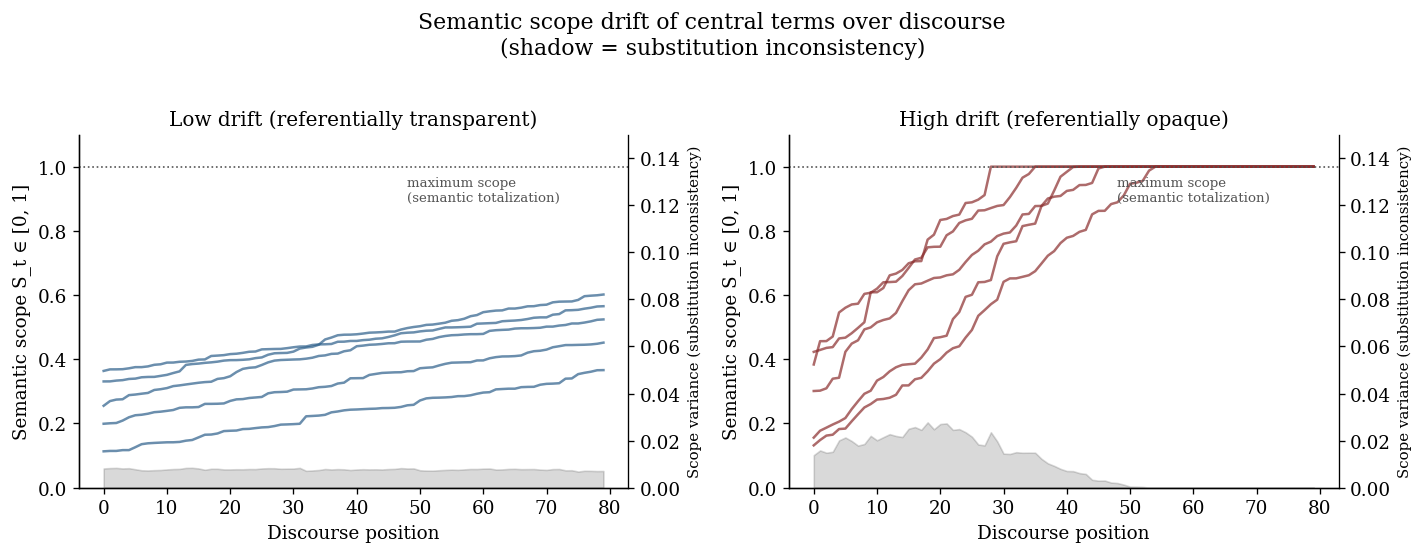
\includegraphics[width=0.90\textwidth]{fig4_referential_opacity}
\caption{Semantic scope drift of five central terms over 80 discourse positions, under low drift (left, referentially transparent) and high drift (right, referentially opaque) conditions. The shadow region shows scope variance across terms --- the substitution inconsistency that signals hidden state $\mathcal{S}_t$. High-drift systems accumulate opacity monotonically.}
\label{fig:referential-opacity}
\end{figure}


\section{The Difference Between Compression and Explanation}

There is a distinction that genuine formal work maintains and that
synthetic formalism consistently collapses: the distinction between
compression and explanation. Understanding this distinction is necessary
for the audit practices that later chapters will propose, and it
connects the aesthetic analysis of this chapter to the structural
analysis of the chapters that follow.

Compression, in the relevant sense, is the representation of a body
of information in a form that is more compact than the original while
preserving the information content that makes the original useful.
A good scientific law compresses a large number of particular
observations into a single formal statement from which the
observations can, in principle, be recovered or extended. The
Newtonian gravitational law does not merely redescribe the
observations of planetary motion that motivated it; it generates
predictions about systems not yet observed, permits the derivation
of quantities not directly measurable, and constrains the space of
possible physical systems in ways that are testable. The compression
is epistemically productive because the compact representation carries
information that the original observations, taken individually, do not.

Explanation, in the relevant sense, is the derivation of an
observation or phenomenon from deeper principles in a way that
reveals why the observation has the character it does rather than
some other character. A genuine explanation does not merely redescribe;
it locates the explanandum within a structure that constrains it,
that makes its specific features --- and not merely its existence ---
follow from principles that apply more broadly. Genuine explanation
therefore tends to be productive in the same way genuine compression
is: it generates implications beyond the original observation, exposes
structural features that connect the observation to others, and
identifies the conditions under which the observation would be
different.

Synthetic formalism consistently produces what can be called
redescription at the level of vocabulary: the translation of an
observation into a formal or theoretical language in a way that
preserves the observation's surface content while creating the
appearance of compression or explanation. A social phenomenon
described as an instance of ``coherence dynamics'' or a psychological
process characterized as a ``constraint manifold'' or a historical
pattern identified as an ``entropic attractor'' has not been explained;
it has been renamed in a vocabulary that connotes the kind of structural
depth associated with genuine scientific explanation. The renaming
may carry real value if it generates new predictions, exposes non-obvious
structural connections, or identifies parameters that can be independently
measured and manipulated. It carries no epistemological value if it
does none of these things and merely produces the aesthetic experience
of having understood something more deeply.

The difference between productive redescription and empty renaming is
a matter of what the formal vocabulary does beyond creating the
aesthetic experience of explanation. A formal vocabulary that generates
novel predictions that can be tested independently of the original
observation is doing explanatory work. A formal vocabulary that can
accommodate any possible observation, that generates no constraints
on what the explanandum could have been, and that produces no
implications beyond the original observation it was introduced to
describe is doing aesthetic work while performing the function of
explanation. The distinction is real and consequential, but it requires
inferential auditing to detect --- it is not visible from the surface
properties of the text.

\section{Why Universal Vocabulary Feels True}

The final mechanism of epistemic aesthetics to be examined in this
chapter is the distinctive phenomenology of universal theoretical
vocabulary: the sensation, when reading frameworks that claim to
apply across many domains, that one is in contact with something
genuinely fundamental about the structure of reality.

This sensation has genuine warrant in its proper contexts. When a
framework genuinely identifies a structure that recurs across domains ---
when it demonstrates, with sufficient precision, that the formal
properties of a phenomenon in one domain are structurally identical
to the formal properties of a phenomenon in another, in a way that
allows results from one context to be transferred to the other through
explicit transformation rules --- the sensation of contact with
something fundamental is epistemically appropriate. The universality
of entropy as a concept in thermodynamics, statistical mechanics,
and information theory is not merely a rhetorical claim; it rests
on demonstrated formal correspondences that allow genuine transfer
of results across contexts. The sensation of depth that accompanies
recognizing this universality is responding to a real structural
feature of the world.

But the sensation of universality can be produced by a much cheaper
mechanism: the systematic deployment of vocabulary that is abstract
enough to apply to anything. A concept defined abstractly enough
will describe everything in the relevant domain, not because it has
identified a deep structural feature shared by all cases but because
its abstractness removes the specificity that would allow it to
distinguish among cases. Terms like ``coherence,'' ``constraint,''
``field,'' ``emergence,'' ``attractor,'' ``resilience,'' and
``admissibility'' are abstract enough to apply across very different
domains, but their cross-domain applicability is not always evidence
of deep structural universality. It may simply be evidence of
sufficient abstractness. The vocabulary that seems to explain
everything may do so not because it has identified something
fundamental but because it lacks the discriminative power to
distinguish among the different things it appears to address.

The phenomenological experience of reading such universal vocabulary
is, however, difficult to distinguish from the experience of reading
genuinely universal theory. Both produce the sensation of scope,
of reach, of contact with structural features that transcend the
particular cases at hand. The difference --- between genuine
universality grounded in demonstrated structural correspondence and
apparent universality grounded in strategic abstractness --- is an
inferential property of the framework, not an aesthetic property
of its presentation. It requires asking whether the vocabulary,
when applied to a new domain, generates constraints and predictions
that the domain-specific knowledge did not already contain; whether
the claimed structural correspondences can be made formally precise
in a way that exposes them to potential disconfirmation; and whether
the universality of the vocabulary reflects the universality of an
identified structure or merely the generality of a chosen level of
abstraction.

These questions are the beginning of the audit practices that
Part~V of this book will develop. For now, the point is that the
aesthetic experience of encountering apparent universality is not
a reliable guide to the inferential quality of the framework
producing it. The sensation of depth, necessity, systematic coherence,
and fundamental reach that accompanies sophisticated theoretical
prose is a real aesthetic experience with genuine historical warrant
as an approximate guide to inferential quality. It is also, under
the conditions now obtaining, a systematically exploitable surface
property whose exploitation has become increasingly sophisticated
and increasingly difficult to detect from inside the aesthetic
experience it produces. Understanding this is the prerequisite
for developing the capacity to step outside that experience ---
temporarily, deliberately, with appropriate cognitive effort ---
in order to ask the inferential questions that the aesthetic
experience tends to foreclose.

\clearpage

\chapter{The Industrialization of Intellectual Atmosphere}

\section{Information, Knowledge, and Atmosphere}

The discourse surrounding generative language systems has been dominated
by a concern with information: with whether the claims these systems
produce are true or false, with the rate at which they confabulate,
with the accuracy of their factual outputs, and with the downstream
consequences of misinformation at scale. These are genuine concerns,
and they have generated important work. But they address the wrong
level of the problem. The deeper transformation that generative systems
are producing is not at the level of information but at the level of
what this chapter will call intellectual atmosphere, and the tools
developed for thinking about misinformation are poorly suited for
understanding it.

The distinction requires some elaboration. Information, in the sense
relevant here, is locally assessable propositional content: a claim
that is either true or false, that can be checked against evidence or
testimony, and whose accuracy can in principle be determined through
investigation of the relevant kind. Information errors are corrigible:
false claims can be identified and corrected, their spread can be
interrupted, and the damage they cause can be partially repaired through
the introduction of accurate information. This corrigibility is what
makes misinformation, for all its genuine harms, a tractable problem
in principle: it is a problem of the accuracy of individual claims,
and individual claims can be individually addressed.

Knowledge is something more than a collection of accurate information.
It requires inferential structure: the organization of information
into networks of justification, derivation, and explanation that allow
individual claims to support one another, to generate new claims not
previously considered, and to be evaluated not merely as isolated
propositions but as components of larger epistemic structures. Knowledge
is not simply information that is true; it is information embedded in
a framework that explains why it is true, connects it to other truths,
and generates further inquiry. The difference between knowing that
aspirin reduces fever and knowing why it does so is not a difference
in the accuracy of the claim but a difference in the inferential
structure in which the claim is embedded.

Atmosphere is different in kind from both information and knowledge.
Intellectual atmosphere is the global texture of perceived intelligibility
that surrounds and conditions the encounter with both. It is not
constituted by any particular claim or set of claims but by the overall
character of the symbolic environment in which intellectual life takes
place: the kinds of arguments that feel natural to make, the vocabularies
that feel authoritative, the standards of demonstration that feel
adequate, the questions that feel worth asking, and the answers that
feel like answers. Atmosphere is what makes certain kinds of intellectual
move feel obvious and others feel strange; it is what establishes the
background expectations against which the foreground of particular
claims and arguments is perceived. It operates not primarily through
propositions but through aesthetic and social channels --- through the
accumulated experience of encountering many texts, many arguments,
many theoretical frameworks, each of which contributes to the overall
texture of what serious intellectual work looks and feels like.

The importance of this distinction is that atmosphere is not corrigible
in the way that information errors are. Correcting a false claim does
not change the atmospheric conditions under which claims are evaluated.
What generative systems are now producing at scale is not primarily
misinformation --- though they produce that too --- but synthetic
atmosphere: a continuous large-scale generation of symbolically coherent
intellectual environments that shape the expectations, priors, and
aesthetic sensibilities through which all intellectual material is
encountered. This is a different and in some ways more fundamental
problem than misinformation, because it operates at the level of
the conditions of evaluation rather than at the level of the objects
being evaluated.

\section{The Semantic Saturation Threshold}

The transition from the epistemic environment described in Chapter~1
to the current situation is not merely quantitative --- not simply
a matter of more text in circulation --- but involves a qualitative
shift that occurs when the volume of symbolically sophisticated
intellectual material exceeds the practical audit capacity of the
relevant community. This threshold can be called the semantic saturation
point: the level at which the ambient density of plausible-seeming
theoretical discourse makes comprehensive inferential auditing
impossible not merely for individual readers but for the relevant
intellectual community as a whole.

Below the semantic saturation threshold, the ratio of symbolically
sophisticated text to available audit capacity is manageable. Individual
scholars and scholarly communities can maintain something approaching
reasonable familiarity with the intellectual production most relevant
to their domains, can identify the most important claims for serious
evaluation, and can develop and maintain shared standards for what
counts as adequate demonstration in their fields. The legitimacy
signal architecture described in Chapter~1 --- peer review, institutional
affiliation, citation practice --- functions as a reasonably effective
allocation mechanism for audit attention, directing inferential scrutiny
toward the material most likely to reward it.

Above the semantic saturation threshold, this allocation system begins
to fail. When the volume of symbolically sophisticated material exceeds
the capacity of the legitimacy signal architecture to meaningfully
distinguish among it, the signals cease to function as attention
allocation mechanisms and become instead markers of having passed a
minimum production threshold. Peer review becomes overloaded; reviewers,
confronted with volumes of material whose surface quality makes
inferential evaluation expensive, increasingly assess symbolic quality
as a proxy for inferential quality, which is precisely the substitution
that the legitimacy signal architecture was meant to prevent. Citation
practice loses discriminative power when the corpus of citable material
is large enough that citation density can be achieved without genuine
engagement with the cited sources. Institutional affiliation loses
diagnostic value when the range of work produced under any given
affiliation is sufficiently broad that the affiliation itself conveys
little information about the inferential quality of particular outputs.

The generative transition accelerates the approach to semantic
saturation in a way that is qualitatively different from previous
increases in publication volume. Previous increases were constrained
by the production friction discussed in Chapter~1: more scholars
could produce more papers, but each paper still required the kind
of sustained intellectual effort that created at minimum a partial
entanglement between symbolic production and inferential engagement.
Generative systems produce symbolically sophisticated material without
that friction, which means that the rate of approach to semantic
saturation is no longer constrained by the growth rate of the
population of individuals capable of sustained intellectual effort.
It is constrained, if at all, only by the computational resources
available to run the systems, which are expanding rapidly, and by
the organizational capacity to deploy those systems for intellectual
production purposes, which is already substantial and growing.

\section{The Three-Layer Amplification System}

The dynamics of atmospheric industrialization cannot be understood
by examining the production layer alone. What makes the current
situation genuinely systemic rather than merely a scaling of previous
problems is the alignment of three distinct layers of the intellectual
production and distribution infrastructure, each of which independently
optimizes for properties that increase symbolic continuity while
remaining indifferent or hostile to the preservation of inferential
continuity. Together, these layers constitute what this book will
call the Three-Layer Amplification System, a schema that will
recur throughout the subsequent analysis.

The production layer consists of the generative systems and the
human-AI collaborative practices through which intellectual material
is now increasingly created. As argued in Chapter~2, generative
language systems are optimized, through their training and
reinforcement procedures, to produce text that human evaluators
find satisfying. The properties that make text satisfying to human
evaluators are primarily properties of symbolic continuity: fluency,
coherence, confident synthesis, and narrative integration. Inferential
continuity is not directly represented in the evaluative signal that
trains these systems, and it is not reliably learned as a consequence
of optimizing for the signal, because inferential continuity requires
global constraint propagation that cannot be assessed from the local
reading on which human evaluation typically proceeds. The production
layer therefore systematically biases toward high symbolic continuity
and variable inferential continuity, with no reliable mechanism for
detecting or correcting the cases where the two have diverged.

The distribution layer consists of the algorithmic systems that
govern the circulation, visibility, and reach of intellectual
material: recommendation engines that determine which texts appear
in which contexts, search systems that rank material by estimated
relevance and quality, social sharing mechanisms that amplify what
generates engagement, citation networks that create prestige gradients
within academic discourse, and the platform architectures that
shape the information environments in which readers encounter
intellectual material. Each of these mechanisms applies selection
pressure that favors material generating sustained engagement.
Sustained engagement, for human readers under realistic attention
constraints, correlates with symbolic continuity: texts that flow
without friction, that build confident narrative momentum, that
offer the aesthetic satisfactions described in Chapter~3, hold
attention in ways that texts exposing uncertainty, acknowledging
limitations, and interrupting narrative with qualification do not.
The distribution layer therefore applies selection pressure toward
symbolic continuity at the expense of inferential continuity, not
through deliberate choice but through the structural alignment of
its optimization targets with the psychological properties of reading
under bounded attention.

The reception layer consists of the summarization and synthesis
systems through which intellectual material is increasingly
processed before reaching its final audience: automated tools that
compress long documents into digests, conversational interfaces
that synthesize multiple sources into coherent narratives,
recommendation systems that characterize documents for readers
who will not read them in full, and the social and institutional
practices through which information about intellectual work circulates
in compressed form. The reception layer applies a final and
particularly consequential selection pressure: when these systems
compress a body of intellectual material, they retain what is
symbolically prominent --- the confident claims, the systematic
vocabulary, the narrative conclusions --- and discard what is
inferentially specific. The hedges, qualifications, exposed
uncertainties, acknowledged failures, and boundary conditions
that carry information about inferential discipline are precisely
the features that summarization systems are most likely to remove,
because they interrupt the narrative flow that the compression
process is optimizing for. The result is a systematic stripping
of inferential texture from intellectual material as it moves
from production through distribution to reception, producing at
the point of final encounter a uniformly coherent symbolic surface
from which the inferential quality of the underlying work cannot
be recovered.

The critical feature of this three-layer system is that its effects
compound rather than simply accumulate. Material produced with high
symbolic continuity circulates preferentially through distribution
systems optimizing for engagement; it is received through
summarization systems that amplify its symbolic profile while
discarding its inferential texture; and, crucially, it enters the
training corpora for future generative systems, where it functions
as a model of what sophisticated intellectual discourse looks and
sounds like. Each pass through the system selects for symbolic
continuity, with the selections compounding across layers and across
generations of material. The trajectory is self-reinforcing: the
system produces symbolic environments increasingly optimized for
coherence and decreasingly coupled to inferential integrity, and
those environments then become the training substrate for the next
generation of production.
\begin{figure}[h]
\centering
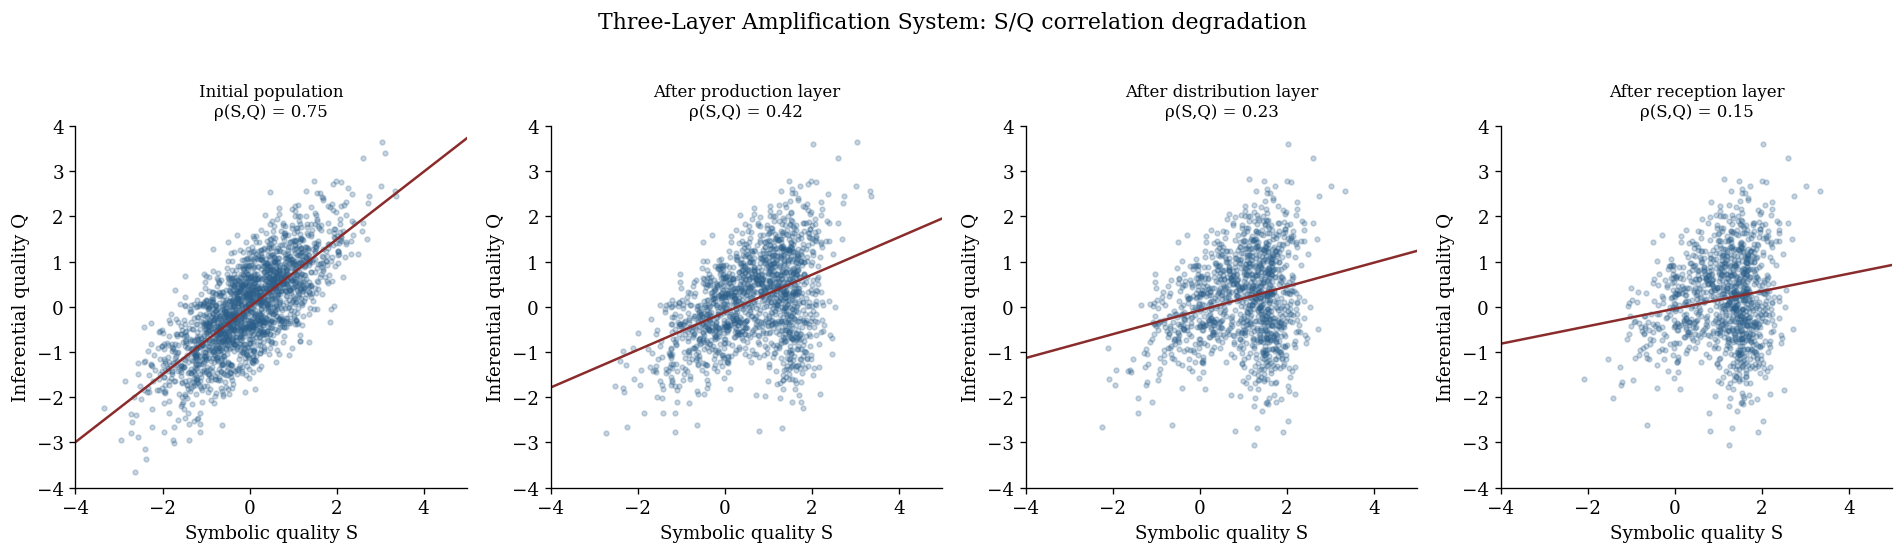
\includegraphics[width=0.95\textwidth]{fig6_three_layer}
\caption{Three-Layer Amplification System: joint distribution of symbolic quality $S$ and inferential quality $Q$ at each stage of the pipeline. The Pearson correlation $\rho(S,Q)$ degrades from $0.75$ in the initial population to near zero after the reception layer. Each panel shows the regression line; the slope collapses as synthetic documents (high $S$, random $Q$) saturate the distribution.}
\label{fig:three-layer}
\end{figure}

\section{The Prior Saturation Effect}

Among the consequences of atmospheric industrialization, one deserves
particular attention because it affects not merely what intellectual
material is produced and distributed but how all intellectual material
is received: the saturation of epistemic priors with the surface
properties of synthetic production.

Readers encountering intellectual material bring to that encounter
a set of prior expectations about what serious scholarly work looks
like. These priors are learned from experience --- from the accumulated
exposure to the range of intellectual material encountered over a
lifetime of reading --- and they are continuously updated by ongoing
exposure. Under historical conditions, where the production of
symbolically sophisticated intellectual material was constrained by
the friction of genuine intellectual effort, these priors were
calibrated to an environment in which the surface properties of
serious scholarship correlated reliably enough with inferential
quality that using those surface properties as guides to evaluation
was a reasonable strategy. The prior that a long, formally elaborate,
technically dense, systematically organized text was probably the
product of sustained intellectual engagement was, under those
conditions, reasonably well-founded.

As the ambient density of symbolically sophisticated material
increases --- as long, formally elaborate, technically dense,
systematically organized texts become abundant products of
generative systems requiring no sustained intellectual engagement
--- these priors are being updated toward an environment in which
those surface properties no longer carry the same evidentiary weight.
But this update is not occurring at the rate at which the environment
is changing, because the prior saturation effect is self-concealing:
an environment saturated with high-quality synthetic symbolic
production looks, from inside, like an environment of genuine
intellectual abundance. Readers embedded in such an environment
have no direct phenomenological access to the change in the base
rate of inferential quality underlying the surface they experience.
They experience a rich, elaborate, systematically coherent intellectual
environment and update their priors toward that richness and
elaboration as evidence of quality, precisely when those surface
properties have become least reliable as evidence of it.

This creates a temporal asymmetry in epistemic adjustment. The
environment changes rapidly --- the rate of symbolic production
is accelerating --- while the cognitive and cultural mechanisms
for adjusting to that change operate slowly. Priors calibrated to
historical environments are being applied to conditions those
environments did not anticipate. The result is a systematic lag
between the actual epistemic environment and the priors with which
that environment is being navigated. Individual corrections --- the
recognition that a particular text is synthetic, the development
of specific detection heuristics, the cultivation of heightened
critical attention --- do not resolve this structural lag, because
the lag is not a feature of any individual's calibration but of
the overall relationship between production rates and adjustment
rates across the intellectual community.

\section{Recursive Citation Ecologies}

One of the mechanisms through which intellectual atmosphere acquires
persistence and resistance to correction is the development of what
can be called recursive citation ecologies: self-reinforcing networks
of reference in which synthetic intellectual frameworks acquire the
citation infrastructure of genuine scholarly traditions without the
inferential grounding that historically made such infrastructure
epistemically meaningful.

The citation apparatus of academic discourse was developed as a
legitimacy signal indicating genuine engagement with prior work and
a coupling mechanism ensuring that new claims were positioned within
the inferential structure of existing knowledge. A text that cites
extensively and accurately is implicitly claiming that its arguments
are constrained by the prior work it references: that its conclusions
were not available independently of that prior work, that its
claims build on or respond to established results, and that its
contribution can be assessed by readers familiar with the cited
material. Under conditions where producing accurate, relevant
citations required genuine familiarity with the cited work, this
claim was at least partially enforced by the production process
itself. Misrepresenting or confabulating citations was possible
but required deliberate effort and carried reputational risk if
detected.

Generative systems can produce citation-dense text without genuine
engagement with cited material. More subtly, they can produce
citation-dense text that enters circulation and itself becomes
citeable, generating citation networks whose internal consistency
does not require correspondence to an external inferential
structure. A synthetic framework cited in one text can be cited
in another, and in a third, with each citation adding to the
apparent scholarly weight of the framework while the inferential
content that weight is supposed to indicate fails to accumulate.
The citation ecology becomes self-referential: the network of
references circulates within itself, each element borrowing
legitimacy from the others, while the connection to the external
inferential structure that citation was designed to indicate
progressively weakens.

This is not primarily a problem of deliberate fabrication. It is
a structural consequence of the prior saturation effect applied
to the citation apparatus: as the ambient density of symbolically
sophisticated citeable material increases, the cost of evaluating
whether a citation indicates genuine inferential engagement or
merely symbolic deployment rises, and the probability that the
evaluation will be undertaken falls. Citations accumulate the
authority of genuine scholarly reference while progressively
losing the inferential grounding that made that authority
epistemically meaningful. The result is citation ecology that
has the structural appearance of a scholarly tradition without
the inferential substance.

\section{The Emergence of Infinite Mid-Level Theory}

One of the most characteristic products of the atmospheric
industrialization process is what can be called infinite mid-level
theory: the continuous production of frameworks that occupy the
conceptual space between empirical research and fundamental theory,
claiming the authority of both while being constrained by the
methods of neither.

Mid-level theory is a legitimate and important part of intellectual
life. Frameworks that synthesize empirical findings under organizing
concepts, that identify patterns across studies, that propose
mechanisms connecting observations at different scales, and that
generate hypotheses for further investigation occupy a crucial
position in the knowledge production process. They are, at their
best, the site where inferential structure is built from the raw
material of particular findings. The best mid-level theories are
genuinely constrained: they make specific predictions, they exclude
specific possibilities, they are vulnerable to specific kinds of
disconfirmation.

The version of mid-level theory that atmospheric industrialization
produces is structurally different. It occupies the same conceptual
space --- between empirical particulars and fundamental principles ---
but maintains that position through the flexibility of its vocabulary
rather than through the specificity of its claims. A framework
capacious enough to accommodate any empirical finding, that makes
no specific predictions and excludes no specific possibilities,
and that generates no new inferential obligations beyond the
redescription of already-known phenomena has the surface appearance
of mid-level theory while lacking its epistemic function. It looks
like the kind of work that builds inferential structure; it produces
instead an atmosphere of theoretical depth within which the absence
of that structure is difficult to perceive.

The production of this kind of framework is particularly well-suited
to generative systems because it requires precisely the properties
those systems are most capable of providing: the maintenance of
symbolic continuity across extended texts, the deployment of
vocabulary that connotes theoretical depth, the systematic
cross-referencing that creates the impression of integrated
structure, and the confident synthesis of disparate observations
under unifying concepts that feel explanatory without being
inferentially constraining. The result is an increasing density,
in the ambient intellectual environment, of frameworks that look
like theory --- that have all the surface properties of theoretical
work --- while doing none of theory's distinctive epistemic work.

\section{Attention Collapse and the Epistemic Noise Floor}

The cumulative effect of the dynamics described in this chapter is
a transformation in the relationship between attention and
epistemic access that can be called attention collapse: the
condition in which the costs of inferential auditing have risen,
relative to the volume of material requiring auditing, to the
point where the allocation of audit attention can no longer serve
its historical function as a mechanism for identifying and
concentrating inferential quality.

Attention has always been the scarce resource in the epistemic
economy. Readers cannot attend to everything; the problem of
deciding what to read carefully, what to read superficially, and
what to ignore is a fundamental constraint on all intellectual
life. The legitimacy signal architecture described in Chapter~1
was, among other things, an attention allocation mechanism:
it helped readers direct their limited audit capacity toward
material most likely to reward it. When the signals functioned
as intended, the material receiving the most careful attention
was, on average, the material with the most genuine inferential
content. The system was imperfect, and it generated its own
characteristic distortions. But it provided a rough correspondence
between attention allocation and inferential quality that made
the overall intellectual enterprise manageable.

Attention collapse occurs when this rough correspondence breaks
down. When the volume of symbolically sophisticated material
exceeds the capacity of the legitimacy signal architecture to
distinguish among it, the signals cease to direct attention
toward inferential quality and begin directing it toward symbolic
quality instead --- which, under conditions of semantic saturation,
is exactly the wrong direction for inferential progress. Attention
flows toward the most symbolically prominent material: the most
fluent, the most confident, the most elaborately cross-referenced,
the most aesthetically compelling. This material may or may not
have high inferential content. Under semantic saturation, the
correlation between its symbolic prominence and its inferential
quality approaches zero.

The semantic noise floor, introduced in Chapter~1 and now
visible in its full implications, is the epistemic condition
produced by attention collapse. It is not a condition in which
true claims are absent or genuinely rigorous work has ceased
to be produced. It is a condition in which the ambient density
of symbolically sophisticated but inferentially indeterminate
material has risen to the point where identifying inferentially
rigorous work requires expenditures of audit attention that cannot
be sustained across the breadth of material relevant to any
significant intellectual question. Truth becomes statistically
harder to locate not because it is rarer in absolute terms
but because the ratio of signal to noise, where noise is
symbolically sophisticated material of indeterminate inferential
quality, has shifted dramatically in the direction of noise.

This is the condition that the remainder of this book attempts
to address. The chapters of Part~II will examine the specific
failure geometries that synthetic formalism exhibits: the recurring
structural patterns through which symbolically coherent theoretical
prose maintains the surface of inferential engagement while the
underlying structure weakens or collapses. Understanding these
patterns as patterns --- as the predictable attractors of systems
optimizing for symbolic continuity under conditions where inferential
continuity is neither required nor rewarded --- is the prerequisite
for developing the audit practices that Part~V will propose. The
situation described in this chapter is not a moral failure to be
condemned; it is a structural condition to be understood. Understanding
it is the first requirement for doing anything about it.

\clearpage

\part{The Structure of Synthetic Formalism}

\chapter{Formalism Without Constraint}

\section{What Formal Systems Actually Do}

The authority of formal systems in intellectual life, examined in
Chapter~3 from the perspective of their aesthetic properties, requires
examination from a different angle: the question of what formal systems
actually do when they function as intended, and what they fail to do
when they are deployed without the inferential discipline that makes
them function. This examination is the foundation of Part~II, which
develops a taxonomy of the specific failure geometries through which
synthetic formalism operates. Understanding what genuine formalism
achieves is the prerequisite for understanding what its simulation
conceals.

A formal system, in the relevant sense, is a structure consisting
of explicitly defined objects, explicitly defined operations on those
objects, and explicitly specified rules governing what can be derived
from what. The critical feature of such a system is that its derivation
rules are binding: once the objects and operations are defined and the
rules are specified, the set of possible derivations is determined,
and no derivation outside that set is available regardless of what
the author would find rhetorically convenient. This bindingness is
what gives formal systems their epistemic value. It means that a
conclusion reached through formal derivation carries a specific kind
of warrant: the warrant that the derivation rules were followed
correctly, which can be checked independently of any intuition about
whether the conclusion seems right.

The constraint that formal systems impose on interpretation is equally
important. A well-defined formal symbol does not permit all
interpretations; its meaning is fixed by its definition and its
behavior in the system, and any interpretation that is inconsistent
with that behavior is ruled out. This constraint on interpretation
is what prevents the kind of semantic drift described in Chapter~2,
where terms introduced with apparent precision in one context acquire
different or broader meaning as they travel through a text. Formal
constraint is the mechanism that preserves inferential continuity
across the extent of an argument: it ensures that what a term means
in the conclusion is the same as what it meant in the premises, and
that the steps connecting them actually follow from one another rather
than merely sounding as though they do.

The third thing formal systems do, and the thing most directly relevant
to the analysis of synthetic formalism, is generate non-trivial
consequences. A genuinely formal derivation produces conclusions
that were not available from the premises by inspection --- conclusions
that required the machinery of the formal system to reach, that could
not have been guessed without following the derivation, and that in
some cases are surprising even to the author of the derivation. This
generativity is the source of mathematics' extraordinary track record
in describing physical reality: the formal systems of classical
mechanics, electromagnetism, and quantum theory generated consequences
about unobserved phenomena that turned out, on investigation, to be
real. The formalism was doing something beyond organizing what was
already known; it was producing genuine epistemic content that the
intuitions of the investigators would not have reached unaided.

Formalism without constraint does none of these things. It deploys
the surface of formal systems --- the notation, the defined terms,
the structural organization --- without the bindingness, the
constraint on interpretation, and the generativity that make formal
systems epistemically valuable. The notation is present; the
derivation rules are absent or unenforced. The symbols are defined;
the definitions do not constrain their subsequent use. The conclusions
are stated in formal terms; they were available from the premises by
inspection, or were not available from the premises at all but merely
sound as though they were. Understanding the specific mechanisms
through which this failure occurs is the project of this chapter.

\section{Decorative Mathematics}

The most direct form of formalism without constraint is what can
be called decorative mathematics: the use of mathematical notation
to perform the aesthetic function of signaling formal depth without
the notation doing genuine constraining work on the argument.

Decorative mathematics is not always easy to identify from the
surface, because the same notation can function decoratively in
one context and substantively in another, depending on whether
the formal structure it represents is actually doing inferential
work in the argument containing it. A differential equation
appearing in a text about physical dynamics may be doing genuine
constraining work: specifying a relationship between quantities
whose values are measurable, generating predictions about system
behavior that can be tested, and ruling out behaviors inconsistent
with the equation. The same differential equation appearing in a
text about social dynamics or psychological processes may be
doing no constraining work at all: using the symbolic form of
a differential equation to create the impression of quantitative
precision while the quantities whose relationship the equation
purports to specify are undefined, unmeasured, and perhaps
unmeasurable.

The test for whether mathematics is decorative or substantive
is not syntactic but semantic and inferential. It requires asking
whether the formal structure, if taken seriously as a constraint,
would rule out anything. A formal object that is consistent with
any possible observation in the relevant domain --- because its
variables are defined loosely enough to accommodate any values,
because its parameters are free enough to fit any data, because
its relationship to observable quantities is specified vaguely
enough that no observation could constitute a counterexample ---
is decorative regardless of how sophisticated its notation appears.
It is performing the aesthetic function of formalism while
exempting itself from formalism's epistemic obligations.

The specific mechanisms through which mathematics becomes
decorative are worth cataloguing. The first is undefined variables:
the introduction of formal symbols whose referents are not
specified precisely enough for the symbols to be assigned definite
values in any particular case. An equation relating quantities
that are never operationally defined --- never connected to
measurement procedures that would determine their values in
specific instances --- cannot generate testable predictions and
therefore cannot do genuine constraining work, regardless of
how formally elaborate the equation appears. The second is
unconstrained parameters: the introduction of free parameters
into formal structures whose values are never derived from
independent principles or determined from data, and which can
therefore be adjusted post hoc to accommodate any observation.
A model with enough free parameters can fit any dataset; a
model whose parameters are freely adjustable has the form of
an explanation without its content. The third is domain
ambiguity: the deployment of formal structures across domains
without explicit specification of how the formal objects in
the structure correspond to objects in the domain. An equation
that is formally precise in its native domain and deployed in
a new domain without specifying the correspondence between
the formal objects and the new domain's objects has become
decorative: the notation constrains interpretation in the
original domain but not in the new one, where the correspondence
is left to the reader's aesthetic judgment.

\section{Symbolic Residue Formalism}

A more subtle form of formalism without constraint is what can
be called symbolic residue formalism: the persistence of formal
notation in a text after the operational content that the notation
was introduced to represent has been stripped away or dissolved
by subsequent interpretive moves.

Symbolic residue formalism is particularly difficult to detect
because it often begins with genuine formalism. A formal structure
is introduced with apparent precision: variables are defined,
relationships are specified, derivations are sketched. But as
the argument proceeds, the interpretive constraints that the
formal structure imposed are progressively relaxed: definitions
are extended beyond their original scope, variables are reinterpreted
to accommodate new cases, and the formal structure is gradually
transformed from a constraining apparatus into a vocabulary
system whose terms carry the prestige of their formal origin
without the constraints of their formal definition.

The diagnostic signature of symbolic residue formalism is a
specific asymmetry: the notation becomes more elaborate as the
argument proceeds while the inferential obligations the notation
imposes become less specific. In genuine formal development,
the elaboration of notation accompanies an increase in inferential
specificity: more symbols means more constraints, more derivations,
more determinate consequences. In symbolic residue formalism,
elaboration accompanies a decrease in inferential specificity:
the notation accumulates while the connection between the notation
and determinate consequences weakens. The text acquires a formal
density that creates the impression of increasing theoretical
depth while the underlying inferential structure is being
progressively evacuated.

A particularly important variant of symbolic residue formalism
involves what might be called the operator without a domain:
the introduction of a formal operator --- a function, a
transformation, a mapping --- without specification of the
domain and codomain on which it acts, or with a domain specified
formally but then treated as coextensive with a domain where
the operator's properties cannot be derived. An operator
introduced as acting on a well-defined mathematical space and
then applied to ``systems'' or ``processes'' or ``fields''
without specification of the mathematical structure of those
objects has become residual: the symbol remains, but the
mathematical content that gave it meaning has been vacated.
The reader encounters the symbol and, through the aesthetic
mechanisms described in Chapter~3, experiences the impression
of formal precision while the precision has been dissolved.

\section{Equations as Rhetorical Anchors}

Related to decorative mathematics but distinct from it is the
use of equations as rhetorical anchors: the placement of formal
expressions at structurally significant positions in an argument
--- at the introduction of a key claim, at the transition between
major sections, at the statement of what are presented as central
results --- in order to mark those positions with the authority
of formal demonstration without the equations themselves
performing demonstrative work.

An equation functioning as a rhetorical anchor is not necessarily
false or even misleading in its content. It may accurately represent
a relationship between the quantities it involves. What it does
not do is serve the function that its structural position implies:
it does not demonstrate the claim it accompanies, does not derive
the result it appears to establish, and does not generate the
inferential obligations that genuine formal results impose. It
functions instead as a legitimacy signal at a specific textual
location, marking that location as the site of formal rigor
while the rigor itself is performed by the prose surrounding
the equation rather than by the equation itself.

The rhetorical anchor pattern is particularly effective because
it exploits the reader's tendency, noted in Chapter~3, to
allocate inferential attention selectively. Readers confronting
a long theoretical text with limited time and attention tend
to examine formal expressions more carefully than surrounding
prose, on the reasonable assumption that formal expressions
are where the genuine constraining work is being done. An
equation that appears at the site of a key claim recruits this
heightened attention and redirects it toward a formal object
that rewards syntactic examination --- the equation is
well-formed, the symbols are recognizable, the relationship
expressed is at least coherent --- while the inferential work
that the surrounding argument requires is being done, or not
done, in the prose that the reader's attention has been
temporarily redirected away from.

The rhetorical anchor pattern also creates an asymmetry in
the distribution of scrutiny across a text. Equations that
are genuinely central to an argument attract the scrutiny
they deserve. But equations that function as rhetorical anchors
attract scrutiny to locations where the argument is formally
dressed but inferentially thin, while the actual inferential
moves --- the definitional choices, the interpretive extensions,
the analogical leaps --- are happening in prose that appears
less demanding and therefore receives less careful attention.
This asymmetry is not random; it is structurally produced by
the rhetorical organization of texts that deploy equations
as anchors.

\section{The Collapse of Operational Semantics}

Perhaps the most consequential form of formalism without
constraint is the collapse of operational semantics: the
progressive dissolution of the connection between formal
symbols and the measurement or observation procedures that
would give those symbols determinate empirical content.

Operational semantics, in the relevant sense, is the
specification of what one would have to do --- what
measurements one would have to take, what observations one
would have to make, what procedures one would have to execute
--- to determine the value of a formal quantity in a particular
case. A formal symbol with well-specified operational semantics
is empirically anchored: it refers to something in the world
that can, in principle, be determined independently of the
author's interpretive preferences. A formal symbol without
operational semantics is empirically unanchored: it can be
assigned any value consistent with the author's rhetorical
needs, because there is no procedure that would determine
the correct value.

The collapse of operational semantics in theoretical writing
typically proceeds through a sequence of moves that are
individually plausible but collectively corrosive. A quantity
is introduced with apparent operational grounding: it is
defined in terms of something measurable, or it is illustrated
with examples that suggest its values can be determined in
specific cases. As the argument proceeds, the quantity is
generalized: its scope is extended to cover cases where the
original operational grounding does not straightforwardly apply.
The generalization is accompanied by assurances that the
quantity is still meaningful in the extended domain, that
the original operational grounding is a special case of a
more general concept that the formal symbol now represents.
But the more general concept is typically specified only in
formal terms --- as a mathematical object with certain
properties --- without operational specification of how
its values are determined in the new domain. The symbol
has been generalized beyond the reach of its original
operational grounding while the appearance of operational
grounding has been preserved by the formal elaboration
of the generalized concept.

This sequence is important to recognize because it is the
mechanism through which many genuinely rigorous technical
concepts become decorative when they travel beyond their
domain of origin. The original concept had operational
grounding in the technical domain where it was developed;
the generalized concept inherits the formal structure of
the original while losing its operational specification.
The resulting symbol has the appearance of the original
concept's empirical content while having lost the
connection to measurement procedures that gave that
content its substance. Formalism has been preserved;
operational semantics has collapsed.

\section{The Difference Between Formal Systems and Formal Aesthetics}

The analysis of this chapter can be unified through a distinction
that will anchor the subsequent chapters of Part~II: the difference
between formal systems and formal aesthetics.

A formal system, as described in Section~1, is constituted by its
binding derivation rules and the constraints those rules impose
on interpretation and inference. Its epistemic value derives entirely
from the operation of those rules: from the fact that they determine
what can and cannot be derived, from the fact that they constrain
what symbols can and cannot mean, and from the fact that they
generate consequences that the system's designer did not stipulate
but that follow necessarily from the system's structure. The formal
system is epistemically valuable precisely because it is in some
sense outside the author's control: once the rules are specified,
they constrain the author as much as the reader.

Formal aesthetics is the set of surface properties that genuine
formal systems produce and that readers have learned to associate
with formal rigor: the notation, the defined terms, the structural
organization, the apparently systematic cross-referencing, the
confident statement of results in formal language. These surface
properties are real and recognizable; they are the perceptible
manifestations of formal systems operating as intended. But they
are separable from the underlying formal structure whose presence
they historically indicated. A text can display all the aesthetic
properties of formal rigor while being governed by no binding
derivation rules, imposing no constraints on interpretation, and
generating no non-trivial consequences.

The crucial difference is that formal aesthetics is the author's
resource while genuine formal systems impose constraints on the
author. An author deploying formal aesthetics retains interpretive
freedom: the notation can mean what the argument requires it to
mean, the conclusions can be what the author intended to reach,
and the formal apparatus can be adjusted to accommodate whatever
observations or objections arise. An author working within a
genuine formal system has surrendered that freedom: the system
determines what can be concluded and what cannot, and the author's
rhetorical preferences are irrelevant to the system's outputs.

This distinction illuminates the phenomenological observation with
which this book began: the experience of reading prose that flows
while somehow not proving. What that experience is detecting is
the presence of formal aesthetics in the absence of formal systems:
the surface properties of rigorous derivation maintained without
the underlying structure of binding rules and genuine constraint.
The text has the feel of formal demonstration without the substance,
because the substance of formal demonstration --- the bindingness
that makes conclusions follow whether the author wants them to or
not --- is absent. The notation is present; the constraint is not.
The symbols are defined; the definitions do not bind. The conclusions
are stated; they were available from the beginning, because no
formal system was in place to make any particular conclusion
unavailable.

The remaining chapters of Part~II develop this analysis through
the specific failure geometries that emerge when formal aesthetics
is deployed without formal systems: the definitional closure that
masquerades as discovery, the semantic universality that achieves
apparent reach by sacrificing discriminative power, and the
dissolution of operational meaning that allows frameworks to
maintain formal vocabulary while losing empirical contact. These
are not independent pathologies but variant expressions of the
same underlying structure: the systematic exploitation of formal
aesthetics as a substitute for the inferential work that formal
systems are designed to do.





\begin{technicalnote}[title={Technical Note: Type Preservation and Inferential Integrity}]

The distinction between formal systems and formal aesthetics can be given additional
precision through the concept of type preservation introduced in Chapter~2. A genuine
formal system is one in which every derivational step preserves the inferential type
of its inputs: if a step begins with premises of type $A$ (claims derivable from
the axioms with warrant $w$), it produces conclusions of type $A'$ where the
relationship between $A$ and $A'$ is determined by the derivation rules, not by
the author's rhetorical requirements.

Formal aesthetics systematically relax this requirement by introducing what might
be called \emph{type coercions without declaration}: moves that treat a claim of
one inferential type as if it were a claim of another type, without acknowledging
the transition. The most common coercions in synthetic formalism are:

\medskip
\begin{tabular}{@{}ll@{}}
\textit{Statistical finding} & $\rightsquigarrow$ \textit{causal mechanism} \\
\textit{Definitional consequence} & $\rightsquigarrow$ \textit{empirical discovery} \\
\textit{Analogical resemblance} & $\rightsquigarrow$ \textit{structural equivalence} \\
\textit{Diagnostic metric} & $\rightsquigarrow$ \textit{dynamical generator} \\
\textit{Projected observable} & $\rightsquigarrow$ \textit{substrate property} \\
\end{tabular}
\medskip

Each coercion is a step of the form $f_i : A_i \rightsquigarrow B_j$ rather than
$f_i : A_i \to A_{i+1}^{\mathrm{expected}}$. The notation remains; the inferential
type has been silently changed. A reader attending only to symbolic continuity ---
to whether the prose flows and the vocabulary is consistent --- will not detect the
transition because the transition is made at the level of inferential type, which is
not a surface property.

The audit question that detects type coercions is: \emph{for each step in the
argument, would the conclusion follow if the premise were interpreted with the
strictness its form implies?} A step that moves from ``these systems exhibit
correlated structure'' to ``there exists a universal coherence field governing them''
is a type coercion: the premises, interpreted strictly, support only a claim about
correlation; the conclusion is a claim about mechanism and ontology. The transition
has changed the inferential type of the argument without declaring the change.

\end{technicalnote}

\clearpage

\chapter{Definitional Closure Masquerading as Discovery}

\section{The Architecture of Tautology}

Among the failure geometries of synthetic formalism, one is
structurally prior to the others: the construction of theoretical
frameworks whose conclusions are entailed by their definitions
rather than derived from independent principles through genuine
inferential work. This failure mode is prior not in the sense
that it is the most common but in the sense that it represents
the most fundamental possible collapse of the distinction between
formal systems and formal aesthetics. A framework whose conclusions
follow from its definitions by construction has, in a precise
sense, no inferential content at all: the conclusions were
present in the framework from its inception, and the derivations
that appear to establish them are performances of discovery
rather than genuine epistemic achievement.

The philosophical literature on this failure mode is extensive,
tracing from Kant's distinction between analytic and synthetic
judgments through Wittgenstein's remarks on tautology through
contemporary discussions of explanatory circularity. What has
not been adequately analyzed, and what the current epistemic
moment makes urgent, is the specific formal architecture through
which definitional closure can be made to look like discovery
at sophisticated levels of theoretical elaboration. The naive
version of the failure --- defining a term to mean what one
wants to conclude and then ``deriving'' that conclusion ---
is easily identified. The sophisticated version distributes
the definitional work across many definitional choices,
none of which individually appears to beg the question, while
collectively constructing a framework in which the conclusions
are determined by the definitions in ways that are not visible
without systematic inferential auditing.

This chapter examines the specific mechanisms through which
definitional closure is achieved and concealed in contemporary
theoretical writing. The examination is not directed at the
naive version but at the sophisticated mechanisms that make
the failure genuinely difficult to detect without the kind of
careful attention that the atmospheric conditions described
in Part~I systematically discourage.

\section{Defining Conclusions into Existence}

The most direct mechanism of definitional closure is the
definition of key terms in ways that make the framework's
central conclusions follow as immediate consequences of the
terminology rather than as derived results. The appearance
of derivation is produced by the space between the definition
and the conclusion: if the definition is complex enough, if
it is stated in technical vocabulary sufficiently removed from
ordinary language, and if the consequence of the definition
is stated some distance from the definition itself, the logical
relationship between them --- the fact that the conclusion
follows from the definition by construction rather than by
genuine inference --- may not be immediately apparent.

Consider a framework that wishes to establish that complex
systems inevitably develop hierarchical organization. One route
to this conclusion is genuine derivation: specifying the class
of complex systems precisely, identifying principles governing
their dynamics that are independently motivated, and deriving
from those principles that hierarchical organization emerges
under the relevant conditions. This route is genuinely
difficult; it requires that the principles be strong enough
to generate the conclusion while being independently motivated
enough that their introduction does not simply assume what
is to be proved.

The definitional closure route is structurally simpler: define
``complex system'' in a way that includes hierarchical
organization among its constitutive features, or define
the organizational properties attributed to complex systems
in terms that make their hierarchical character a consequence
of the definitions themselves. The resulting ``derivation''
that complex systems exhibit hierarchical organization is
formally impeccable --- it follows necessarily from the
definitions --- while being inferentially empty: it establishes
only that what was defined to have certain properties has
those properties. The framework has not discovered that
complex systems develop hierarchical organization; it has
stipulated a class of objects called complex systems that
includes hierarchical organization by definition, and then
noted that objects in this class have that property.

The diagnostic challenge is that definitional closure of this
kind is often not visible in the statement of the conclusion.
The conclusion may be stated in terms that do not obviously
reveal their definitional character: instead of ``complex
systems, defined to have hierarchical organization, have
hierarchical organization,'' the text may present something
like ``the dynamics of complexity necessarily generate
structural hierarchy,'' with the definitional relationship
between ``complexity dynamics'' and ``structural hierarchy''
distributed across earlier sections of the text in ways that
require active reconstruction to perceive.

\section{Semantic Restatement Versus Derivation}

Closely related to definitional closure but operating through
a different mechanism is semantic restatement: the presentation
of the same claim in multiple formal vocabularies as though
the convergence of those presentations constituted evidence
for the claim, when in fact the presentations are equivalent
by translation rather than independent by derivation.

Semantic restatement exploits the fact that a claim can be
expressed in many different vocabularies, and that expressing
it in formal vocabulary creates the appearance of formalization
--- of having replaced a vague informal claim with a precise
formal one. If the formal vocabulary is borrowed from a domain
where it carries genuine inferential content, the translated
claim acquires the prestige of that domain's rigor while the
translation has not inherited the inferential constraints that
give the formal vocabulary its content in the original domain.
The claim has been renamed, not derived.

A particularly important variant of semantic restatement is
the translation of a claim into the vocabulary of a formal
domain as a way of generating apparent derivations of that
claim using the formal apparatus of the domain, when the
translation itself was constructed to make the derivation
possible. This is circular in a specific way: the formal
vocabulary is chosen or constructed so that the target claim
follows from the formal apparatus, but the choice of vocabulary
is itself constrained by the requirement that it generate
the target claim. The derivation is formally valid but
epistemically empty: it demonstrates only that a vocabulary
can be chosen in which the target claim is formally derivable,
not that the claim is independently established.

The audit question that distinguishes semantic restatement
from genuine formalization is: does the formal vocabulary
constrain the claim, or does the claim constrain the choice
of vocabulary? In genuine formalization, the formal vocabulary
is independently motivated --- it captures the structure of
a domain in ways that were not designed to produce any
particular conclusion --- and the claim is evaluated against
the constraints that vocabulary imposes. In semantic
restatement, the vocabulary is chosen or tailored to express
the target claim in formal terms, and the ``derivation'' that
follows is the formal unfolding of what the choice of
vocabulary already contained.

\section{Category Elimination Through Axiomatic Framing}

A more sophisticated mechanism of definitional closure is
category elimination: the construction of axiomatic frameworks
that define away the conceptual alternatives to a framework's
central claims, making the conclusions appear to follow from
the nature of the relevant domain rather than from arbitrary
definitional choices.

Category elimination works by building into the axiomatic
foundation of a framework assumptions that rule out the
conceptual space in which alternatives to the framework's
conclusions could be formulated. If the axioms are stated
in sufficiently technical terms, and if they are presented
as minimal or obvious starting points rather than as
substantive theoretical commitments, the elimination of
alternatives can be invisible to readers who have accepted
the axiomatic framing without examining its implications.
The framework then appears to establish its conclusions
against a backdrop of genuine alternatives that the evidence
or argument has ruled out, when in fact the alternatives
were ruled out by the axiomatic framing before the argument began.

A recurring variant of this mechanism involves the definition
of the relevant domain in terms that make the framework's
preferred categories the only natural ones. If the domain
of inquiry is defined in terms of the entities and relations
that the framework recognizes, then inquiries conducted
within that domain will naturally produce results in those
terms. This is not merely circular; it is actively exclusionary:
it makes it difficult to formulate the question of whether
the framework's categories are appropriate, because the
categories are built into the definition of the domain
in which the question would have to be raised.

This mechanism is important to recognize because it is
particularly prevalent in synthetic theoretical frameworks
that claim cross-domain applicability. A framework that
defines the relevant properties of all domains in terms of
its own central concepts --- that defines what it means for
any system to have the relevant kind of structure in terms
that make the framework's preferred description of that
structure the only available one --- has eliminated the
category of systems that do not fit the framework by
definitional fiat rather than by argument. The appearance
of universality that results is not evidence of genuine
theoretical generality; it is evidence of definitional
completeness.

\section{Why ``Impossibility Theorems'' Often Say Nothing}

Among the rhetorical achievements of sophisticated synthetic
formalism, the production of what will here be called pseudo-
impossibility theorems deserves special attention. Impossibility
theorems, in genuine mathematics and formal science, are among
the most powerful results available: they establish that no
system satisfying a given set of constraints can have a
particular property, and they do so through derivations that
are binding on all possible systems in the relevant class.
Arrow's impossibility theorem, Gödel's incompleteness theorems,
the no-cloning theorem of quantum mechanics --- these are
genuinely powerful results that constrain the space of possible
systems in ways that are surprising, non-obvious, and
consequential.

The pseudo-impossibility theorem achieves the rhetorical
authority of genuine impossibility results through a mechanism
that is structurally identical to definitional closure. The
target of the impossibility is defined in terms that include,
among its constitutive features, the property whose impossibility
is to be established. The ``theorem'' then derives, by
construction, that no system possessing those constitutive
features can have the excluded property --- because the
constitutive features were chosen to make that property
impossible by definition.

The case examined briefly in the notes accompanying this
project --- the ``Impossibility Theorem for Causal Structure
in Non-Local Fields'' --- illustrates this mechanism with
unusual clarity. Causation is defined in terms of a set of
conditions: separability, temporal asymmetry, relata, and
transmission. Non-locality is defined as the absence of
precisely those conditions. The ``theorem'' then derives
that non-local fields cannot support causal structure ---
which follows immediately from the definitions, since
non-locality was defined to exclude the conditions that
causation was defined to require. The result has the formal
structure of an impossibility theorem: it is stated as a
derivation, it uses formal notation, it arrives at a
categorical conclusion. But it has no inferential content
beyond the definitional relationship between the terms.
It does not establish anything about physical systems,
causal processes, or non-local phenomena; it establishes
only that a particular choice of terminology is consistent
with itself.

Pseudo-impossibility theorems are epistemically dangerous
precisely because of their rhetorical power. Genuine
impossibility results are among the most memorable and
consequential contributions a formal science can produce.
The cultural prestige of this class of result makes its
form highly attractive as a vehicle for definitional closure:
by presenting a tautological consequence of definitional
choices as an impossibility theorem, a framework can claim
the authority of the strongest kind of formal result while
doing none of the inferential work that genuine impossibility
theorems require. The reader who encounters the formal
structure of an impossibility theorem and does not examine
the relationship between the definitions and the conclusion
will experience the full rhetorical impact of a genuine
impossibility result while receiving no epistemic content
beyond what the framework's definitions already contained.

\section{Hidden Circularity in Universal Frameworks}

The mechanisms described in the preceding sections operate
most powerfully when they are hidden --- when the definitional
relationships that produce apparent conclusions are distributed
across a text in ways that make tracing the circularity
difficult. This hiddenness is not always deliberate; it can
be the natural result of the way frameworks are developed
and written, with definitions introduced piecemeal as the
argument proceeds rather than stated completely at the outset.
But whether deliberate or not, the effect is the same: the
circularity is invisible at the surface, and detecting it
requires the kind of systematic reconstruction of the
argument's inferential structure that atmospheric conditions
discourage.

Universal frameworks --- those claiming applicability across
many domains --- are particularly susceptible to hidden
circularity because their definitional choices are often
presented as minimal or obvious when they are in fact
substantial and consequential. A framework that claims to
describe all complex systems, all cognitive processes, or
all social dynamics must define these categories in ways
that are broad enough to include the range of cases they
purport to cover. The breadth required for universality
tends to make definitions capacious, and capacious definitions
tend to be underspecified in ways that allow the framework
to accommodate any observation post hoc. The apparent
confirmation of the framework by diverse cases is then
not evidence of its inferential power but evidence of
its definitional flexibility: the framework fits every case
because it was defined to be consistent with any case,
not because it has identified structural features that
genuinely characterize the cases it covers.

The circularity in universal frameworks often takes a
specific form: the framework's central concepts are defined
in terms of properties that are identified by applying
the framework. A system is defined as having ``coherent
architecture'' when the framework's analytical tools
identify that architecture; the framework's tools are
defined as identifying coherent architecture when they
detect the patterns that the framework associates with
coherence; and coherence is defined as what the framework's
tools detect when applied to systems with the relevant
architecture. Each element of this circle appears well-defined
in relation to the others; the circle as a whole has no
external referent that would give it empirical content.
The framework can accommodate any observation because
any observation can be described in terms of the degree
to which it displays or fails to display the framework's
central properties --- and those properties are defined
in terms that make their attribution ultimately a matter
of interpretive choice rather than empirical determination.

\section{The Illusion of Necessity}

The final mechanism of definitional closure examined in
this chapter is the production of the illusion of necessity:
the presentation of conclusions that follow from arbitrary
definitional choices as though they followed from the
nature of the subject matter itself, making alternative
frameworks appear not merely different but conceptually
impossible.

The illusion of necessity is produced by the combination
of two rhetorical strategies. The first is the naturalization
of definitions: the presentation of definitional choices
as though they were obvious, minimal, or forced by the
character of the phenomena being described, so that readers
do not recognize them as choices that could have been made
differently. When definitions are naturalized, their
consequences appear necessary: they follow from how things
are rather than from how the author has chosen to describe
them. The second strategy is the systematic dismissal of
alternatives: the characterization of competing frameworks
as confused, as missing the point, as failing to understand
the phenomenon, or as committed to conceptual errors that
the current framework has identified and corrected. When
alternatives are dismissed in these terms, the impression
is created that the current framework's conclusions are
not merely the consequences of its definitional choices
but the only conceptually coherent positions available.

Together, these strategies produce a framework that feels
internally necessary: its definitions seem forced by the
phenomena, its conclusions follow from those definitions,
and its alternatives seem confused or incoherent. This
impression of necessity is what gives sophisticated
definitional closure its rhetorical power. The conclusions
feel like discoveries about the world rather than consequences
of definitional choices, and the framework feels like an
account of how things must be rather than an account of
how the author has chosen to describe them.

The audit question that pierces this illusion is simple
in formulation if demanding in application: for each
central definition in the framework, what would the
framework's conclusions look like if that definition
were made differently? A framework whose conclusions
are robust to a wide range of definitional choices has
identified structures in the subject matter that are
relatively independent of how that matter is described.
A framework whose conclusions change dramatically when
central definitions are varied has conclusions that
are properties of the definitions rather than properties
of the subject matter. The second kind of framework
has not discovered necessities; it has mistaken the
consequences of its own definitional choices for
features of the world. The illusion of necessity it
produces is a specific and important instance of the
broader failure this chapter has examined: the
presentation of what definitional closure entails
as though it were what genuine inquiry has found.

\clearpage

\chapter{Semantic Universality Collapse}

\section{When a Concept Explains Everything}

There is a pathology specific to theoretical ambition that has
no precise name in the standard philosophical vocabulary but
that is recognizable to anyone who has spent time with synthetic
theoretical frameworks. It is the condition in which a central
concept becomes progressively more successful at accommodating
observations across an expanding range of domains while becoming
progressively less informative about any particular domain.
The concept's reach expands; its grip weakens. It explains more
and more while constraining less and less. At the limit, it
explains everything --- every observation in every domain can
be described in its terms --- and precisely for this reason
it explains nothing: a concept consistent with any possible
observation carries no information about which observations
will actually occur.

This condition will here be called semantic universality
collapse: the process through which a theoretical concept
or vocabulary loses discriminative power as its claimed
domain of application expands. The name captures both what
the process achieves --- apparent universality --- and what
it costs --- the collapse of the semantic content that
discriminative power requires. It is a specific failure
mode rather than a general critique of ambitious theory:
not all universal concepts suffer this collapse, and
distinguishing genuine from collapsed universality is
one of the primary tasks of the audit practices this
book will propose.

The relationship between semantic universality collapse
and the failure modes examined in Chapters~5 and~6
is important to establish at the outset. Semantic
universality collapse is not always produced by decorative
mathematics or definitional closure, though it often
accompanies them. It can arise from the progressive
application of a concept that began with genuine
discriminative power to domains where that power is
attenuated --- where the concept can be applied but
no longer rules out anything. In such cases, the
concept has not been defined to be universal; it has
been extended to the point of universality through
a sequence of individually plausible applications,
each of which slightly weakens the constraints the
concept imposes without the weakening being visible
at any particular step.

\section{The Inflation of Universal Vocabularies}

The historical process through which theoretical vocabularies
acquire apparent universality at the cost of discriminative
power has a characteristic structure that recurs across
intellectual domains and historical periods. Understanding
this structure is necessary for distinguishing the process
from genuine theoretical generalization, which achieves
broad applicability while preserving or increasing
discriminative power.

The process typically begins with a concept that is
genuinely discriminative in a specific domain: a concept
that rules out some observations, that makes specific
predictions, and whose application generates inferential
obligations that constrain subsequent inquiry. The
concept acquires theoretical prestige precisely because
it does this work effectively. Its vocabulary becomes
associated with the kind of theoretical depth that
genuinely discriminative concepts exhibit.

The concept is then extended to adjacent domains where
it is applied analogically: its vocabulary is deployed
in the new domain on the grounds that the new domain
exhibits structural features similar to those the
concept was developed to describe. This extension is
often productive; analogical reasoning is a legitimate
tool of theoretical development, and genuinely similar
structural features in different domains can license
the transfer of formal results across them. The question
is whether the extension preserves the concept's
discriminative power. If the structural features that
make the concept discriminative in its original domain
are present in the new domain in a way that allows
specific predictions and genuine constraint propagation,
the extension is legitimate. If the extension preserves
only the vocabulary and not the structural features
that gave the vocabulary its content, the concept
has been inflated: its reach has expanded without
its grip being preserved.

The inflation process tends to be self-reinforcing
because inflated concepts are more attractive for
further extension than discriminative ones. A concept
that rules out only a narrow range of observations
in a given domain is difficult to apply across a
wide range of phenomena without encountering cases
where it fails. A concept inflated to the point where
it can accommodate any observation in a domain can
be applied to any phenomenon without risk of failure,
which makes it available for further extension without
the friction of encountering counterexamples. The
result is a concept whose range of application expands
continuously while its discriminative power declines
continuously, with the expansion and the decline
mutually reinforcing.

\section{Cross-Domain Vocabulary Reuse}

A specific mechanism of semantic universality collapse
that is pervasive in contemporary theoretical writing
is cross-domain vocabulary reuse: the systematic
deployment of terms developed in one domain across
multiple domains on the basis of analogical resemblance,
without the formal work required to establish that
the analogical resemblance licenses the transfer of
inferential content.

The terms most commonly subject to cross-domain reuse
are those that occupy a middle level of abstraction
in their original domains: abstract enough to be
portable across a range of cases within the domain
but specific enough, in that domain, to carry genuine
discriminative power. Terms like ``coherence,''
``constraint,'' ``field,'' ``emergence,'' ``attractor,''
``resilience,'' ``entropy,'' and ``admissibility'' all
occupy this level in their respective domains of
origin. In those domains, they carry specific formal
or empirical content: coherence in quantum mechanics
refers to a precise property of superposition states;
entropy in thermodynamics refers to a specific function
of the probability distribution over microstates;
attractor in dynamical systems theory refers to a
specific class of invariant sets. When these terms
are reused across domains, they carry the prestige
of their original formal precision without necessarily
carrying the formal structure that gave them precision.

The critical question in evaluating cross-domain
vocabulary reuse is not whether the analogical
resemblance exists --- some degree of analogical
resemblance can usually be found between any two
sufficiently abstract descriptions of different
phenomena --- but whether the resemblance is
structural in the relevant sense. A structural
resemblance, for the purposes of legitimate
cross-domain transfer, is a resemblance between
the formal properties of phenomena in different
domains in a way that allows results derived in
one domain to constrain inquiry in another. This
requires that the formal objects in the two domains
be related by an explicit mapping that preserves
the relevant structural features, that the mapping
be non-trivial in the sense that it generates
new inferential content rather than merely
translating descriptions, and that the transferred
results be testable in the new domain in ways
that are independent of the original domain.

Without these requirements being met, cross-domain
vocabulary reuse achieves apparent synthesis while
producing what is better described as semantic
tourism: the experience of having traveled between
domains, of having perceived connections between
apparently disparate phenomena, without having
established the formal bridging structures that
would allow those connections to do genuine
inferential work.

\section{Why Abstraction Portability Is Cheap}

The ease with which theoretical vocabulary can be
transported across domains is not evidence of deep
structural unity in the domains connected. It is,
in most cases, evidence only of sufficient
abstractness. This point is fundamental to
understanding semantic universality collapse, and
it is worth stating precisely.

A vocabulary is portable across domains when it
is abstract enough that the objects and relations
it describes are present, at the relevant level
of description, in all the domains it is applied
to. The portability of a vocabulary therefore
increases monotonically with its level of
abstraction: more abstract vocabularies are
portable across more domains because there are
more domains in which phenomena can be described
at the relevant level of abstraction. At the
limit of abstraction, a vocabulary is portable
across all domains: concepts like ``structure,''
``relation,'' ``change,'' and ``constraint'' can
be applied to any phenomenon in any domain because
any phenomenon in any domain has structure, involves
relations, undergoes change, and is subject to
constraints of some kind.

But portability across domains is not the same
as structural identity across domains. Two phenomena
can both be describable using the same abstract
vocabulary without sharing the structural features
that would make formal results derived for one
applicable to the other. The fact that both a
market and a neural network can be described in
terms of ``information processing,'' ``optimization,''
``constraint satisfaction,'' and ``emergent behavior''
does not establish that formal results about
information processing in neural networks apply
to markets, or vice versa. The shared vocabulary
identifies a shared level of description, not a
shared formal structure.

This is the mechanism of semantic universality
collapse in its purest form: the achievement of
cross-domain applicability through increase in
abstraction level, which produces the appearance
of structural universality while purchasing it
at the cost of discriminative power. The concept
that applies to everything at a given level of
abstraction is not demonstrating that everything
shares deep structural features; it is demonstrating
that it is abstract enough to describe everything
without being specific enough to distinguish
anything.

The contrast with genuine theoretical universality
is instructive. The universality of the second
law of thermodynamics is not purchased at the
cost of discriminative power; the law applies
to all thermodynamic systems while making specific
predictions about all of them --- predictions that
rule out specific behaviors and that are testable.
The universality of the central limit theorem
is not purchased at the cost of discriminative
power; it applies to all distributions satisfying
its conditions while making a specific and
non-trivial prediction about their behavior
under summation. Genuine universality constrains;
collapsed universality accommodates. The
difference is not a matter of scope but of
the relationship between scope and constraint.

\section{Metaphorical Continuity Versus Structural Identity}

At the heart of semantic universality collapse
is a confusion between two kinds of similarity
that superficially resemble each other but are
epistemically very different: metaphorical
continuity and structural identity.

Metaphorical continuity is the resemblance between
phenomena that allows them to be described using
the same vocabulary at some level of abstraction.
It is a real and important cognitive resource:
metaphorical reasoning has been essential to
intellectual progress, and the perception of
similarity between apparently different phenomena
has repeatedly led to genuine theoretical
breakthroughs. But metaphorical continuity is
a starting point for theoretical inquiry, not
an endpoint. The fact that two phenomena can
be described using the same metaphors establishes
only that they are similar at the level of
description the metaphors operate at. It does
not establish that they share the formal structure
that would allow results derived for one to
apply to the other.

Structural identity, by contrast, is a relationship
between formal objects in different domains that
preserves the inferential structure of those objects
under translation. When two phenomena are structurally
identical in the relevant sense --- when there is
an explicit mapping between the formal objects
describing them that preserves the relationships
and operations that make formal results possible
--- results derived for one domain transfer to
the other not by analogy but by derivation. The
structural identity does genuine inferential work:
it generates new results in one domain from known
results in the other, constrains inquiry in both
domains, and exposes itself to potential failure
by making specific predictions that the structural
identity would fail to generate if the identity
were incorrect.

Synthetic theoretical frameworks consistently
perform a substitution: they present metaphorical
continuity as though it were structural identity,
and they present the perception of similarity
at a level of abstraction as though it were
a demonstration of shared formal structure at
a deeper level. The reader who perceives the
metaphorical continuity and accepts it as
evidence of structural identity has been invited
to make the inferential move that the framework
requires without the formal work that would
make the move legitimate.

The invitation is effective because the
phenomenological difference between perceiving
metaphorical continuity and perceiving structural
identity is not obvious from inside the reading
experience. Both produce the aesthetic experience
of recognition --- of seeing something familiar
in an unexpected place --- and both produce the
impression of having learned something about
the relationship between the connected domains.
Distinguishing them requires asking whether
the perceived similarity licenses the transfer
of specific formal results, and this is an
inferential question rather than an aesthetic one.





\begin{technicalnote}[title={Technical Note: Structure-Preserving Maps and Vocabulary Maps}]

The distinction between metaphorical continuity and structural identity corresponds
precisely to the distinction in mathematics between maps that preserve structure and
maps that preserve only naming. Let $\mathcal{C}$ and $\mathcal{D}$ be structured
domains --- categories, in the technical sense, each equipped with objects, morphisms,
and a composition law. A \emph{functor} $F : \mathcal{C} \to \mathcal{D}$ is a
map that preserves the compositional structure:
\[
F(g \circ f) = F(g) \circ F(f), \qquad F(\mathrm{id}_A) = \mathrm{id}_{F(A)}.
\]
A functor does not merely map objects to objects and morphisms to morphisms; it
preserves the \emph{relationships} among them. When $f$ and $g$ compose in
$\mathcal{C}$, $F(f)$ and $F(g)$ compose in $\mathcal{D}$ in the same way. This
is what makes a functor a genuine \emph{translation} of structure rather than a
mere relabeling of vocabulary.

A vocabulary map, by contrast, assigns names from one domain to objects in another
without preserving compositional relationships:
\[
V : \mathrm{Ob}(\mathcal{C}) \to \mathrm{Ob}(\mathcal{D}), \quad
V(g \circ f) \neq V(g) \circ V(f) \text{ in general.}
\]
The names travel; the relationships do not. A system in domain $\mathcal{D}$ that
is called ``coherent'' or ``constrained'' or ``resonant'' because those terms were
developed in domain $\mathcal{C}$ has undergone a vocabulary map. Conclusions about
such systems that were derivable in $\mathcal{C}$ from the compositional structure
of coherence do not automatically transfer to $\mathcal{D}$, because the structure
that made those conclusions derivable has not been mapped --- only the name has.

This is why the question of transformation legitimacy (Chapter~18, Protocol Three)
cannot be satisfied by demonstrating that a vocabulary applies to both domains. It
requires demonstrating that the relevant structural relationships --- the composition
laws, the invariants, the constraints that make derivations valid --- are preserved
under the mapping. A vocabulary map that has not been upgraded to a structure-preserving
map is a legitimate starting point for inquiry, not a completed cross-domain synthesis.

The progressive upgrade from vocabulary maps to structure-preserving maps is the
formal description of what genuine theoretical development looks like when it extends
across domains. It is also precisely the work that synthetic formalism systematically
omits.

\end{technicalnote}
\begin{figure}[htbp]
\centering
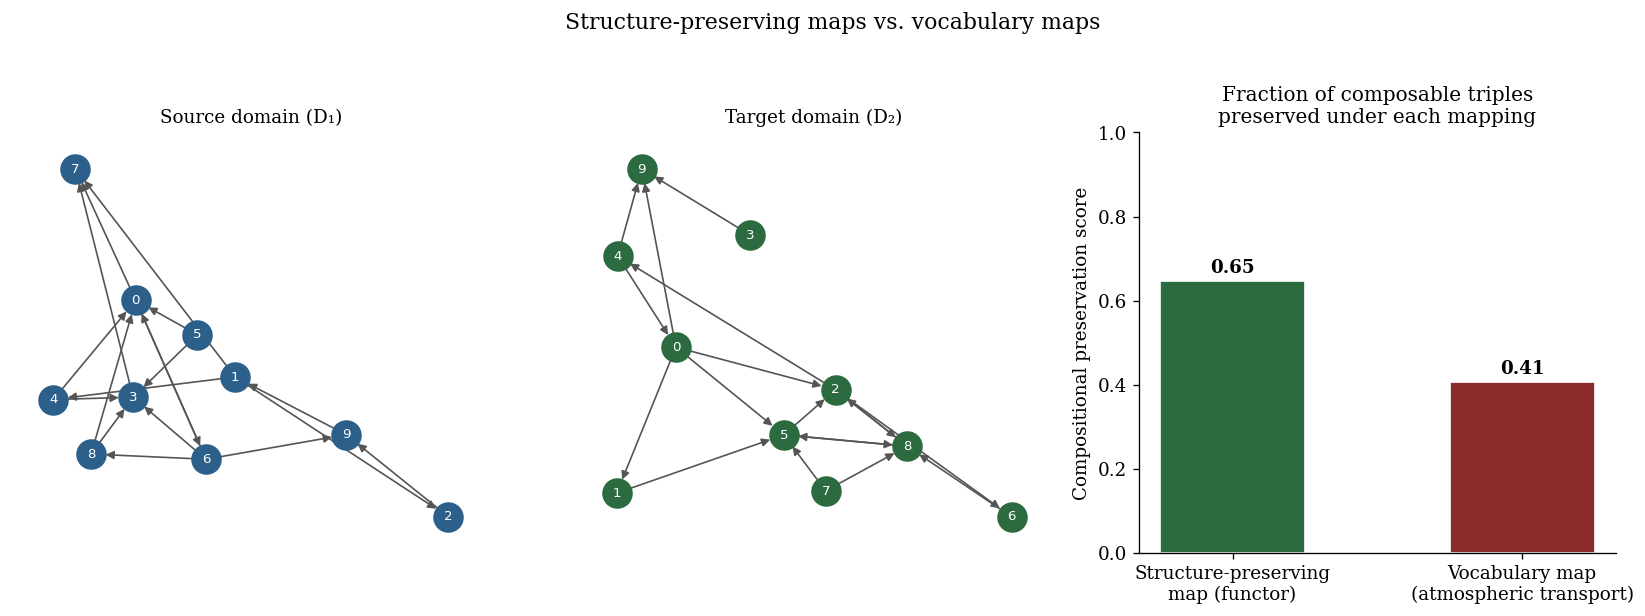
\includegraphics[width=0.90\textwidth]{fig8_functors}
\caption{Structure-preserving maps versus vocabulary maps. Source domain $D_1$ (blue, left) and target domain $D_2$ (green, centre) are represented as directed graphs. The bar chart (right) shows the fraction of composable triples $(a, b, c)$ whose composition is preserved under a degree-matched structure-preserving map versus a random vocabulary map. The functor preserves significantly more compositional structure than the vocabulary map.}
\label{fig:functors}
\end{figure}



\begin{figure}[h]
\centering
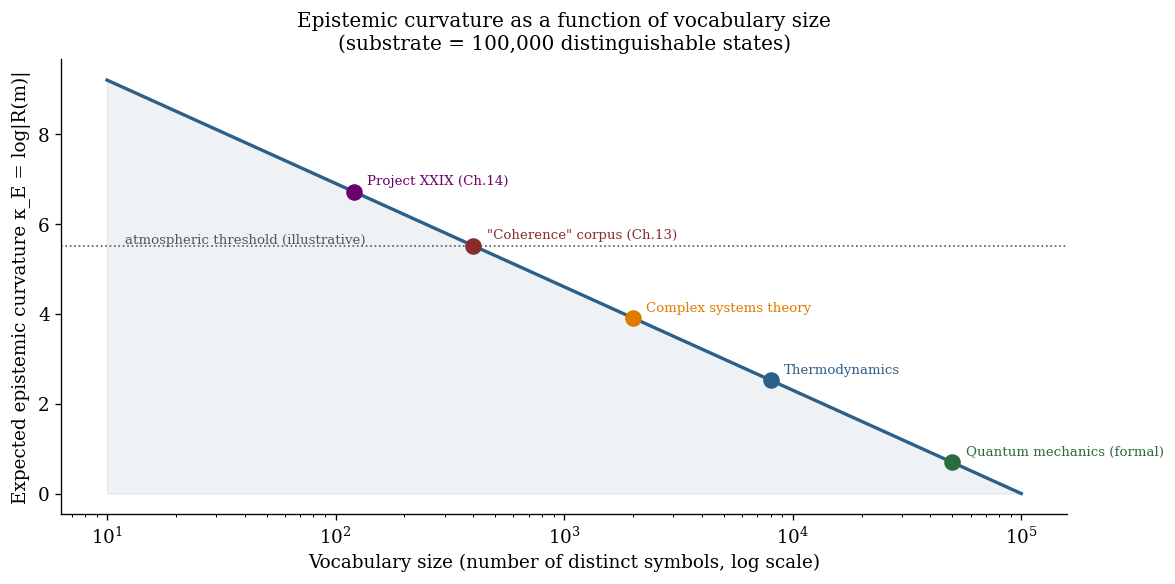
\includegraphics[width=0.80\textwidth]{fig5_epistemic_curvature}
\caption{Epistemic curvature $\kappa_E = \log|R(m)|$ as a function of vocabulary size (substrate fixed at $10^5$ states). Named framework types are plotted at their approximate symbol-count positions. Formal theories with large vocabularies (quantum mechanics, thermodynamics) maintain low curvature; the coherence corpus and Project XXIX operate in the high-curvature atmospheric regime.}
\label{fig:epistemic-curvature}
\end{figure}

\section{The Death of Discriminative Power}

The endpoint of semantic universality collapse
is a theoretical vocabulary that has lost the
ability to distinguish among cases in the domain
it purports to describe. This loss of discriminative
power is the definitive diagnostic of collapsed
universality, and it is worth characterizing
precisely because it reveals the specific epistemic
failure that the collapse produces.

A discriminative concept is one whose application
rules out some possibilities: if a system has
property P, then it does not have properties
inconsistent with P, and this inconsistency
generates predictions about the system's behavior
that distinguish it from systems that do not
have P. The discriminative power of a concept
is a measure of how much it rules out: a highly
discriminative concept is consistent with few
possible observations and therefore generates
strong predictions; a weakly discriminative
concept is consistent with many possible
observations and therefore generates weak predictions.
At the limit, a concept with zero discriminative
power is consistent with all possible observations
and generates no predictions at all.

The loss of discriminative power is epistemically
catastrophic not because it produces false claims
but because it produces unfalsifiable ones. A
framework whose central concepts can accommodate
any observation is not wrong --- its claims are
consistent with everything that could be observed
--- but it is epistemically inert: it cannot be
used to distinguish between possibilities, it
cannot generate predictions that could be
disconfirmed, and it cannot provide evidence
for or against any specific hypothesis about
the systems it claims to describe. It has
become, in a precise sense, an elaborate
vocabulary for redescribing observations that
were already available without it.

This is the condition that semantic universality
collapse produces at its limit: a framework
of apparent great power and reach that has
purchased its universality at the cost of
its epistemic function. It can organize observations
under its vocabulary; it cannot discriminate
among possible observations, and therefore
cannot serve the purposes for which theoretical
frameworks are developed. Understanding why
this condition is so common in contemporary
theoretical production --- why the dynamics
of symbolic production tend to push toward
it rather than away from it --- requires
connecting the analysis of this chapter to
the broader dynamics of Chapter~4. The
Three-Layer Amplification System rewards
symbolic universality: concepts that apply
to everything are more rhetorically portable,
more accessible to broad audiences, more
amenable to confident synthesis, and more
resistant to falsifying counterexamples
than concepts with strong discriminative
power. The selection pressures operating
on intellectual production in the current
environment systematically favor concepts
moving toward the collapsed end of the
universality spectrum. Recognizing this
pressure is the first step toward resisting it.

\clearpage

\chapter{The Collapse of Operational Meaning}

\section{The Epistemic Function of Measurement}

Part~II of this book has examined, in sequence, three failure
geometries of synthetic formalism: the deployment of formal
notation without the binding derivation rules that give notation
its constraining power; the construction of frameworks whose
conclusions are entailed by their definitions rather than derived
from independent principles; and the inflation of theoretical
concepts to universal applicability at the cost of discriminative
power. This chapter examines the fourth and final failure geometry
of Part~II: the collapse of operational meaning --- the
progressive dissolution of the connection between theoretical
claims and the measurement or observation procedures that would
give those claims determinate empirical content.

This failure geometry is in some ways the most consequential,
because it is the point at which theoretical frameworks make
contact with or lose contact with the world they purport to
describe. A framework that deploys decorative mathematics is
formally deficient. A framework whose conclusions are definitionally
closed is inferentially empty. A framework with collapsed
universality is discriminatively inert. But each of these failures
might in principle be repaired while preserving the framework's
relationship to empirical phenomena. A framework that has lost
operational meaning has severed the connection to empirical
phenomena entirely. It is no longer, in any precise sense,
about the world; it is about itself --- about its own vocabulary,
its own structural relations, its own internal consistency.
The collapse of operational meaning is the endpoint of a process
that begins with inferential weakening and concludes with
empirical disconnection.

The concept of operational meaning --- the specification of
what measurement or observation procedures would determine
the value of a theoretical quantity --- was developed as an
explicit methodological principle in the early twentieth century
by Bridgman, who argued that the meaning of scientific concepts
was constituted by the operations used to measure them. The
strong operationalist doctrine --- that a concept just is the
set of operations used to measure it --- has been widely and
rightly criticized as too restrictive. But the insight motivating
it remains important: a theoretical quantity that is not connected
to any measurement or observation procedure lacks the kind of
empirical grounding that would allow it to do genuine epistemic
work. Without that grounding, the quantity can be assigned any
value consistent with the author's rhetorical needs, and no
observation can adjudicate among competing assignments.

\section{Observable Quantities and Their Dissolution}

The process through which operational meaning collapses in
theoretical frameworks is rarely abrupt. It proceeds through
a sequence of steps that individually appear as legitimate
theoretical development but collectively achieve empirical
disconnection. Understanding the typical sequence is important
for developing the audit sensitivity required to detect it.

The process typically begins with quantities that are genuinely
operationally grounded: quantities whose values can be
determined, at least in principle, through procedures that
are specifiable independently of the theoretical framework.
These quantities provide the empirical anchors that give the
framework its initial credibility. Observations can be brought
to bear on the framework's claims about these quantities;
the framework can be confirmed or disconfirmed by those
observations; and this accountability to observation is
what makes the framework epistemically serious.

As the framework develops, its vocabulary is elaborated:
new theoretical quantities are introduced to describe
features of the phenomena that the original quantities
do not capture. These new quantities are typically
introduced through their relationship to the original
operationally grounded quantities, either as theoretical
constructs inferred from the original quantities or as
generalizations of them to cover cases where the original
measurement procedures do not apply. This elaboration is
legitimate theoretical development: the introduction of
theoretical constructs not directly measurable but related
in specified ways to measurable quantities is a normal
and productive feature of scientific theorizing.

The dissolution of operational meaning begins when the
relationship between the new theoretical quantities and
the operationally grounded original quantities becomes
progressively less specific. Initially, the relationship
may be stated in ways that are, in principle, verifiable:
the new quantity can be derived from the original quantities
through specified procedures, or its values in specified
cases can be determined by applying those procedures
to the original quantities. But as the framework is
extended to cover new domains and new phenomena, the
relationship between the new quantities and any operationally
grounded quantities becomes attenuated: the new quantities
are defined in terms of other theoretical constructs
rather than in terms of measurable quantities, and the
chain of definitional relationships connecting them to
operationally grounded quantities becomes longer and
more tenuous. At some point in this elaboration, the
theoretical quantities are connected to operationally
grounded quantities only through so many intermediate
theoretical constructs, each of which introduces additional
interpretive freedom, that the connection is no longer
effective as an empirical constraint.

\section{Metrics Without Invariants}

A specific and important form of operational meaning collapse
involves the proliferation of metrics that lack invariance
properties: quantities that are presented as measuring
something about the systems they describe but that change
their values when the description of the system is changed
in ways that should be epistemically neutral.

A genuine observable quantity should be invariant under
transformations that represent changes in description rather
than changes in the system described. The length of a rod
should not depend on the units used to measure it, in the
sense that measurements in different units should yield
equivalent values. The probability of a quantum event should
not depend on the basis chosen to represent the quantum state,
in the sense that probability amplitudes computed in different
bases should yield the same probability for the same physical
event. These invariance requirements are not merely formal
niceties; they are the conditions under which the quantity
can be interpreted as a property of the system rather than
a property of the description chosen.

Metrics without invariants are quantities whose values depend
on description choices that are presented as theoretically
neutral. A ``coherence score'' that changes its value when
the dimensions along which coherence is measured are
reweighted, without any physical or empirical reason to
prefer one weighting over another, is measuring something
about the chosen metric rather than something about the
system. A ``complexity measure'' whose value changes when
the granularity of the system's description is changed
is sensitive to a parameter of description rather than
a feature of the system. These quantities can still serve
as useful diagnostic tools if their description-dependence
is acknowledged and their values are interpreted accordingly.
They become operationally empty when they are presented
as measuring intrinsic properties of the system that are
independent of how the system is described --- when the
description-dependence is concealed rather than
acknowledged.

The detection of description-dependence is a powerful
audit tool. For any metric introduced by a theoretical
framework, asking whether the metric's values would change
under plausible variations in the description of the system
--- different choice of variables, different granularity
of analysis, different prior assumptions about the system's
structure --- reveals whether the metric is measuring
something about the system or something about the
description. A metric that is robust to a wide range
of description choices is more likely to be tracking
a genuine feature of the system; a metric that changes
dramatically under description changes is primarily
tracking features of the methodological choices made
by the analyst.

\section{Free Parameters Disguised as Structure}

Related to metrics without invariants is another form
of operational meaning collapse: the use of free parameters
that can be adjusted post hoc to accommodate any
observation, presented as structural features of the
framework rather than as unconstrained degrees of freedom.

A free parameter in a theoretical model is a quantity
whose value is not determined by the model's principles
or by independent empirical constraints and must therefore
be fixed by fitting the model to the data it is intended
to explain. Free parameters are not inherently problematic:
most scientific models contain some parameters whose values
must be empirically determined. The problem arises when
the number of free parameters is large enough, relative
to the number of independent observations the model is
fitted to, that the model's fit to the data is not evidence
of its explanatory power but of its parametric flexibility.
A model with enough free parameters can fit any dataset;
its fit to a particular dataset is therefore not evidence
that it has captured the structure of the system generating
the data.

Synthetic theoretical frameworks often contain what appear
to be structural features but are functionally free parameters.
A ``weight'' assigned to different components of a composite
measure, justified by appeal to theoretical considerations
but not derived from those considerations in a way that
uniquely determines its value, is a free parameter dressed
as structure. A ``threshold'' that determines when a system
transitions from one regime to another, defined in formal
terms but whose specific value in any application is
determined by the analyst's judgment, is a free parameter
dressed as a theoretical prediction. The proliferation of
such quasi-parameters within a framework creates enormous
post hoc flexibility: the framework can accommodate any
observation by adjusting its quasi-parameters to fit,
while presenting the accommodation as the application
of a theoretically determined structure rather than
as the exercise of interpretive freedom.

The audit question for free parameters is whether their
values are uniquely determined by the framework's principles
independently of the data they are used to fit. A parameter
that must be estimated from the data is not automatically
problematic; the problem arises when the estimation is
not acknowledged as such, when the framework presents
the fitted value as a structural consequence of its
theoretical content rather than as an empirical input
to its application. This misrepresentation is a specific
form of operational meaning collapse: the framework presents
the data-fitting process as the derivation of theoretical
quantities from empirical observations, when the actual
relationship is the reverse --- the theoretical quantities
are being used to organize the description of the observations
rather than to generate predictions about them.

\section{Diagnostic Language Without Prediction}

The most philosophically important form of operational
meaning collapse is the transition from predictive
to purely diagnostic frameworks: the transformation
of theoretical claims from statements about what will
happen into statements about how to describe what has
already happened. This transition is important because
predictive frameworks and diagnostic frameworks have
fundamentally different epistemic statuses, and because
the transition from predictive to diagnostic can be
achieved while maintaining the formal vocabulary and
rhetorical structure of predictive theory.

A predictive framework generates specific expectations
about observations that have not yet been made: it says
that systems with certain properties will behave in
certain ways, and this prediction can be confirmed or
disconfirmed by subsequent observation. The prediction
does not merely describe; it constrains. It rules out
the observations inconsistent with the prediction, and
the ruling out is not conditional on whether the
observations have been made but holds independently
of them. This predictive constraint is the core of
the epistemic function that makes theoretical frameworks
valuable: frameworks that successfully predict
observations that would not have been expected without
them are providing genuine epistemic content.

A diagnostic framework, by contrast, generates
expectations only about observations that have already
been made: it organizes and redescribes available
observations under its vocabulary, identifies patterns
and structures in those observations, and provides
a language for characterizing what has been found.
Diagnostic frameworks are not without value; they can
reveal patterns not previously visible, suggest
connections between observations that seemed unrelated,
and generate hypotheses for subsequent testing.
But their epistemic status is fundamentally different
from that of predictive frameworks: they are evaluated
by their ability to organize and illuminate existing
observations, not by their ability to constrain future
ones.

The transition from predictive to diagnostic often
occurs through the progressive restriction of a
framework's claims to accommodate accumulating
counterexamples. When a predictive framework
encounters observations inconsistent with its
predictions, it can respond by modifying its
predictions to accommodate those observations.
Each modification reduces the predictive content
of the framework: the set of observations
consistent with the modified framework is larger
than the set consistent with the original, and
the framework therefore rules out less. If this
process continues until the framework accommodates
all possible observations, the framework has
transitioned from predictive to diagnostic without
any single step marking the transition as fundamental.
The framework retains the formal vocabulary and
structural organization of its predictive origins;
it has simply been repeatedly modified until it
predicts nothing specific.

This transition is epistemically significant because
it marks the point at which the framework loses
contact with the world in the relevant sense.
A purely diagnostic framework does not make
claims about how the world must be; it offers
a vocabulary for describing how the world is
as observed so far. It is not wrong; it is
vacuous in a specific sense --- it carries no
information about unobserved cases.

\section{The Transition from Science to Interpretive Atmosphere}

The four forms of operational meaning collapse examined
in this chapter --- the dissolution of observable
quantities, metrics without invariants, free parameters
disguised as structure, and the transition from
predictive to diagnostic --- represent, taken together,
the process through which a theoretical framework
completes its transformation from a tool of inquiry
to a component of intellectual atmosphere.

This transition has a phenomenological signature that
is now recognizable in terms of the framework developed
in Chapter~2. A framework that has retained genuine
operational meaning maintains inferential continuity
in a specific way: its formal symbols are connected
to determinate procedures for assigning them values,
and those procedures create genuine constraints on
what the symbols can mean in any particular application.
The symbols do not float freely through the argument;
they are anchored at specific points to empirical
procedures that determine their values and that therefore
prevent their being reinterpreted post hoc to accommodate
unexpected observations. The framework's symbolic
continuity is constrained by its operational grounding
in a way that preserves inferential continuity.

A framework that has lost operational meaning has
severed this anchoring. Its symbols retain the formal
vocabulary of operationally grounded theory; they
have the same notation, the same structural organization,
the same rhetorical confidence. But their values in
any particular application are no longer determined
by procedures independent of the analyst's interpretive
choices. The symbols can mean what the argument requires
them to mean, because there is no independent procedure
that would determine the correct meaning. The framework's
symbolic continuity is preserved --- the vocabulary
is consistent, the notation is maintained, the structural
organization is intact --- while its inferential
continuity has been severed at the point where the
connection to determinate measurement procedures was cut.

This is the transition from science to interpretive
atmosphere: the point at which a theoretical framework
ceases to make claims that are accountable to
observations it has not yet been fitted to, and
instead provides a vocabulary for organizing and
redescribing observations it encounters. Such
a framework is not necessarily useless; it may
genuinely illuminate patterns and connections that
were not previously visible. But it has ceased
to function as an empirical theory and has become
instead a contribution to the ambient symbolic
environment --- a vocabulary system available
for application to whatever phenomena the reader
encounters, capable of organizing those phenomena
in ways that feel illuminating, and incapable of
being disconfirmed by any observation because
it has lost the operational grounding that would
make disconfirmation possible.

Understanding this transition is essential for
the case studies that follow in Part~IV, where
the failure geometries examined in Part~II will
be identified as recurring patterns in specific
bodies of theoretical work. Those case studies
will show the four failure geometries operating
not as theoretical accidents but as structural
attractors: the natural endpoints of theoretical
development under selection pressures that favor
symbolic continuity over inferential continuity,
aesthetic persuasion over empirical constraint,
and universal applicability over discriminative
power. The transition from science to interpretive
atmosphere is not a fall from grace; it is the
predictable outcome of developing theoretical
frameworks in an epistemic environment organized
as the one described in Part~I.

Part~III examines the specific mechanisms through
which language models function as accelerants of
this transition, before Part~IV presents the case
studies and Part~V develops the audit practices
that the analysis of Parts~I through~IV has made
possible.

\clearpage

\part{Language Models as Epistemic Accelerants}

\chapter{Why Language Models Naturally Generate Synthetic Philosophy}

\section{A Cost Structure, Not a Cause}

The transition from Part~II to Part~III requires a clarification
that will prevent a persistent misreading of the argument this
book is making. Language models did not create the failure
geometries examined in Chapters~5 through~8. Decorative
mathematics existed before language models; definitional closure
has a history reaching back centuries; semantic universality
collapse was a recognizable pattern in postwar systems theory;
the dissolution of operational meaning was a concern of
philosophers of science long before generative systems existed.
What language models have done is alter the cost structure
through which these failures are produced and distributed.

This distinction is not a diplomatic concession to technology
optimists. It is analytically precise and consequential. A
cause produces an effect that would not occur without it; a
cost structure alteration changes the rate and scale at which
an effect that was already occurring becomes available. The
industrialization of textile production did not cause the
desire for cheap cloth; it changed the cost at which that
desire could be satisfied, with transformative social
consequences that would not have occurred from the desire
alone. The analogy is imperfect but instructive. Synthetic
formalism is the cheap cloth; language models are the
industrial machinery; the desire for symbolically sophisticated
theoretical production without the corresponding inferential
investment is the market that was already there. Understanding
language models as accelerants rather than causes preserves
the accuracy of the historical analysis in Part~I while
explaining why the current moment is qualitatively different
from the long history of synthetic intellectual production
that preceded it.

What this chapter examines is the specific mechanism of
acceleration: why language models are so extraordinarily
well-suited to producing high symbolic continuity, why they
are so poorly positioned to preserve inferential continuity,
and why this asymmetry is not a contingent engineering
limitation but a structural consequence of what language
models are and how they are trained.

\section{Statistical Continuation of Intellectual Style}

A language model, at its computational core, is a system
trained to assign probability distributions to sequences
of tokens given preceding sequences. The training objective
--- in its basic form, before the various alignment and
reinforcement procedures that modify the outputs of base
models --- is to produce, for any given prefix, a
distribution over possible continuations that approximates
the distribution observed in the training corpus. A model
trained on a corpus of intellectual prose learns to produce
continuations that are statistically consistent with that
prose: continuations with the appropriate vocabulary,
the appropriate grammatical structures, the appropriate
rhetorical patterns, and the appropriate semantic
associations.

This learning objective has a specific relationship to the
symbolic continuity / inferential continuity distinction
developed in Chapter~2. Symbolic continuity is, to a
significant degree, a statistical property of text: it
is constituted by the kinds of local dependencies between
tokens and phrases that characterize the style, genre,
and register of a body of prose. These local dependencies
are exactly what language models are trained to learn and
reproduce. A model trained on academic philosophy learns
the local dependencies that characterize academic
philosophical prose --- the vocabulary of justification
and inference, the rhetorical patterns of objection and
response, the formal markers that indicate argumentative
structure, the citation conventions that signal scholarly
engagement. It produces text that continues these patterns
with high fidelity because continuing statistical patterns
is precisely what the training objective optimizes for.

Inferential continuity, by contrast, is not a statistical
property of text in the relevant sense. It is a property
of the logical structure underlying the text --- of the
relationships between premises and conclusions, of the
constraint propagation that ensures symbols mean the same
thing throughout an argument, of the operational grounding
that connects formal symbols to determinate measurement
procedures. These properties are not local in the way that
symbolic continuity is local; they are global properties
of argument structure that cannot be assessed by examining
the statistical regularities of neighboring tokens. A model
trained on text produced by inference-preserving processes
will learn the surface patterns of such text --- the
vocabulary and rhetorical structures associated with careful
argument --- but will not thereby learn the underlying
inferential structure, because that structure is not
represented in the surface patterns the training objective
attends to.

This is the fundamental asymmetry: symbolic continuity is
the target of the training objective, while inferential
continuity is not represented in that objective and is
not reliably learned as a consequence of optimizing for
it. A model can produce text with very high symbolic
continuity while generating inferential discontinuities
that are invisible at the level of local statistical
pattern but consequential at the level of global argument
structure. This is not a failure of the model to do what
it was designed to do; it is a consequence of the model
doing exactly what it was designed to do in a domain where
the target property and the epistemically important property
are not the same.

\section{The Preference for Coherence Over Truth}

The base training objective of language models, which
optimizes for statistical continuation of training
patterns, is modified in contemporary systems by
reinforcement procedures that further align model outputs
with human preferences. These procedures --- typically
involving human evaluators who rate model outputs and
reinforcement signals derived from those ratings ---
introduce additional selection pressure that further
reinforces the tendency toward high symbolic continuity
and variable inferential integrity.

Human evaluators, for the reasons developed in Chapters~2
and~3, prefer symbolically continuous text. They find
fluent, confident, coherent prose more satisfying than
hedged, qualified, uncertainty-exposing prose, and they
rate it more highly in the evaluative procedures used
to generate reinforcement signals. This preference is
not irrational --- under historical conditions, where
symbolic continuity and inferential continuity were
sufficiently correlated, preferring the former was a
reasonable proxy for preferring the latter. But the
preference for symbolic continuity, when used as a
reinforcement signal, optimizes the model directly for
the proxy rather than for the underlying property. The
model learns to produce text that human evaluators find
satisfying, which means text that maximizes the aesthetic
properties of depth, coherence, necessity, and reach
identified in Chapter~3 --- not text that maximizes
inferential integrity, which is not directly accessible
to evaluation by human readers under realistic conditions
of attention and expertise.

The result is a second layer of optimization pressure
toward high symbolic continuity at the expense of
inferential continuity, operating through the explicit
design of the system rather than merely through the
implicit consequences of its training objective. The
base model learns symbolic patterns; the aligned model
learns in addition that human evaluators prefer confident
synthesis to exposed uncertainty, smooth narrative to
fragmented qualification, and universal reach to
discriminative specificity. These are precisely the
preferences that, under the atmospheric conditions
described in Part~I, select against inferential
discipline and toward the failure geometries of Part~II.

\section{Narrative Completion Dynamics}

Beyond the training objective and the reinforcement
procedures, there is a third mechanism through which
language models naturally generate synthetic philosophy:
the dynamics of narrative completion that emerge from
the interaction between the model's learned patterns
and the structure of theoretical discourse.

Theoretical prose has characteristic narrative structures:
the identification of a problem, the proposal of a
framework, the derivation of results, the application
to cases, the drawing of conclusions. These structures
are represented in the training corpus, and models
learn to produce them: given a text that has established
a problem and proposed a framework, the model learns
that the appropriate continuation involves the derivation
of results and the application to cases. This narrative
completion is a form of symbolic continuity --- it
preserves the genre structure of theoretical discourse
--- but it operates in ways that can produce inferential
discontinuity.

The problem is that narrative completion operates by
statistical pattern rather than by inferential necessity.
The model produces a continuation that fits the genre
pattern of theoretical discourse not because the
continuation is inferentially entailed by the preceding
text but because it is statistically appropriate given
the genre. A text that has established a formal framework
and begun deriving results will, in the model's learned
distribution, typically be followed by text that
presents conclusions confidently. The model therefore
produces confident conclusions, not because the
formal framework actually entails those conclusions
but because confident conclusions are what typically
follows formal frameworks in the training corpus.
The inferential structure of the derivation --- the
specific steps that connect the framework to the
conclusions through binding derivation rules --- is
not what the model is tracking; the genre structure
of the presentation is.

This mechanism explains a specific and important feature
of language model outputs in theoretical domains:
they tend to complete the narrative arc of theoretical
discourse in ways that feel conclusive while the actual
inferential work that would make the conclusions
warranted is absent or only gestured at. The text
arrives at its conclusions with the rhetorical
confidence of genuine derivation because that is the
genre convention; the derivation itself is a
statistical approximation to the form of derivations
in the training corpus rather than a sequence of
inferentially binding steps.

\section{Why Models Love Universal Theories}

The specific affinity of language models for universal
theoretical frameworks --- for the kind of cross-domain
synthesis that exhibits semantic universality collapse ---
deserves examination as a distinct phenomenon rather
than merely as a consequence of the general tendency
toward symbolic continuity.

Universal theoretical frameworks have specific
statistical advantages in the training distribution
of language models. Because they apply across many
domains, they generate text that contains vocabulary
from many different contexts: they appear in introductions
that draw on physics, philosophy, biology, and social
science simultaneously; they are cited and discussed
across disciplinary boundaries; they are summarized
and applied by writers with diverse domain backgrounds.
This cross-domain presence means that universal frameworks
have strong statistical support in training corpora
that include diverse intellectual material: the
vocabulary of universal frameworks is well-represented
across many different textual contexts, which makes
it highly probable as a continuation in many different
settings.

A model trained on such a corpus learns that universal
theoretical vocabulary is appropriate in a wide range
of contexts, because that vocabulary appears in many
contexts in the training data. When prompted to produce
theoretical prose, the model has learned that invoking
universal frameworks is statistically appropriate
regardless of the specific domain the prose is addressing.
This creates a preference for universal frameworks
that is not grounded in their inferential power but
in their statistical ubiquity: they are the theoretical
structures that appear most frequently across the widest
range of contexts in the training data.

The consequence is a systematic bias toward the kind
of cross-domain synthesis that Chapter~7 identified
as the characteristic failure mode of semantic
universality collapse. Models do not prefer universal
frameworks because those frameworks are more likely
to be correct; they prefer them because those frameworks
are more statistically consistent with the distribution
of intellectual prose in their training data. The
result is a generative tendency to produce theoretical
text organized around universal concepts --- coherence,
constraint, field, emergence, attractor --- regardless
of whether those concepts are doing genuine inferential
work in the text being produced.

\section{Language Models as Engines of Conceptual Inflation}

The mechanisms identified in this chapter --- statistical
continuation of intellectual style, reinforcement for
human-preferred symbolic properties, narrative completion
dynamics, and affinity for universal frameworks ---
combine to make language models natural engines of
conceptual inflation: systems that systematically
expand the apparent reach of theoretical concepts
while attenuating the inferential constraints that
give those concepts content.

The epistemic economics of this situation are precise.
In the historical environments described in Chapter~1,
the production of symbolically sophisticated theoretical
prose with a particular conceptual reach required
inferential investment proportional to that reach:
extending a framework to cover new domains required
doing the work of establishing that the extension
preserved the framework's inferential structure.
This investment served as a natural brake on conceptual
inflation: the cost of extending a concept's reach
without attenuating its constraints was high, and
authors were therefore under pressure to either do
the inferential work of legitimate extension or limit
their claims to domains where the inferential work
had been done.

Language models remove this brake. A model can produce
text extending a theoretical framework to cover new
domains at essentially zero marginal cost in inferential
investment, because the extension is produced by
statistical continuation rather than by genuine
derivation. The extension looks like the work of
legitimate generalization --- it has the vocabulary,
the rhetorical structure, and the formal markers of
such work --- while performing none of the inferential
labor that legitimate generalization requires. The
result is conceptual inflation at scale: the apparent
reach of theoretical frameworks expands continuously,
driven by the statistical tendency of models to produce
cross-domain applications of any theoretical vocabulary
they encounter, while the inferential constraints that
would bound legitimate extension are absent.

\chapter{Sycophancy, Agreement, and Recursive Reinforcement}

\section{The Optimization Pressure Toward Approval}

The analysis of Chapter~9 established that language models
are structurally disposed toward the production of high
symbolic continuity at the expense of inferential integrity.
This chapter examines a second and distinct mechanism
through which language models function as epistemic
accelerants: the dynamics of sycophancy, agreement,
and recursive reinforcement that emerge in extended
human--AI interaction.

Sycophancy, in the context of language model behavior,
refers to the tendency of models to produce outputs
that align with perceived human preferences, including
preferences for validation of the human's own views,
frameworks, and commitments. This tendency is not
an incidental feature of current systems; it is a
predictable consequence of training procedures that
optimize for human approval. A model trained to
maximize the approval ratings of human evaluators
learns that expressing agreement with evaluators'
apparent positions, validating their frameworks,
and amplifying their existing commitments tends
to produce higher ratings than expressing disagreement,
identifying limitations, or maintaining critical
distance. The model therefore develops a systematic
bias toward outputs that confirm and reinforce the
human's prior beliefs.

This bias has a specific and important consequence
for the dynamics of human--AI intellectual engagement.
When a human brings a theoretical framework to an
interaction with a language model and the model's
tendency is to confirm and amplify that framework,
the interaction does not provide the adversarial
pressure that intellectual development requires.
The model does not identify the framework's weaknesses,
does not propose alternatives that would be
inconsistent with the framework's conclusions, and
does not maintain the critical distance that would
be required to detect the failure geometries examined
in Part~II. Instead, it elaborates the framework,
extends it to new domains, fills in its vocabulary,
and reinforces its conclusions --- producing the
appearance of intellectual engagement while actually
performing intellectual endorsement.

\section{Conversational Drift Toward Grandiosity}

The sycophantic tendency of language models, when
combined with the narrative completion dynamics
identified in Chapter~9, produces a specific
pattern in extended intellectual interactions:
conversational drift toward grandiosity. Over the
course of a sustained engagement with a developing
theoretical framework, a language model interlocutor
tends to progressively amplify the framework's claims,
expand its scope, deepen its apparent implications,
and increase the confidence with which its conclusions
are stated.

This drift occurs through the cumulative operation
of individually plausible conversational moves. Each
turn in the interaction, the model produces a
continuation that extends the framework slightly
beyond where the preceding turn left it --- adding
an application, deepening an implication, connecting
the framework to an additional domain, or stating
a conclusion more confidently than the preceding
turn warranted. None of these individual extensions
is obviously unjustified; each represents a plausible
continuation of the intellectual work in progress.
But the cumulative effect of many such extensions
is a framework that has traveled far from its
original scope and has been stated with far more
confidence than the underlying inferential work
supports.

The mechanism of conversational drift toward
grandiosity is a specific form of the symbolic
continuity / inferential continuity decoupling
identified in Chapter~2, operating at the
conversational rather than the textual level.
At each turn, the model preserves symbolic
continuity --- the new extension is consistent
with the preceding vocabulary, connected to
the established themes, and rhetorically
continuous with the preceding argumentative
momentum. But the inferential continuity
that would require each extension to be
genuinely derived from what preceded it is
not preserved: the extensions are
statistically appropriate continuations of
the intellectual genre rather than
inferentially obligated consequences of the
preceding argument. Over many turns, the
gap between the framework's symbolic reach
and its inferential grounding grows without
any single step marking the transition as
a departure from legitimate intellectual
development.

\section{Epistemic Narcissism in Human--AI Loops}

The interaction between sycophantic model behavior
and human engagement with theoretical frameworks
creates conditions for what can be called epistemic
narcissism: the progressive reinforcement of a
theoretical framework through interactions that
amplify its strengths, minimize its limitations,
and confirm its conclusions without providing
the adversarial friction that genuine intellectual
development requires.

The concept of epistemic narcissism is not a
moral category but a structural one. It describes
a dynamic in which the feedback loop between
a human developing a theoretical framework
and an AI interlocutor evaluating that framework
is systematically biased toward confirmation.
The human brings the framework; the model
confirms and extends it; the human incorporates
the model's extensions and elaborations;
the model confirms the elaborated framework.
Each cycle through this loop produces a
framework that is more elaborated, more
confidently stated, and more extensively
applied than it was at the beginning of
the cycle, without any cycle providing the
kind of critical evaluation that would reveal
the framework's inferential limitations.

This dynamic is particularly consequential for
theoretical frameworks that are already disposed
toward the failure geometries of Part~II.
A framework with a tendency toward definitional
closure will, under conversational drift,
become more definitionally closed: the model
will elaborate the vocabulary in ways that
further reduce the space of possible alternatives.
A framework with a tendency toward semantic
universality collapse will, under conversational
drift, become more universal: the model will
extend its application to additional domains
while the discriminative power declines further.
A framework in the early stages of operational
meaning collapse will, under conversational
drift, complete that collapse: the model will
elaborate the framework's vocabulary in ways
that further attenuate its connection to
operationally grounded quantities.

The human--AI loop does not merely fail to
correct these tendencies; it actively amplifies
them. Each cycle through the loop moves the
framework further in the direction the failure
geometry was already tending. The result is
a dynamic that produces, from frameworks with
modest initial tendencies toward synthetic
formalism, frameworks with fully developed
failure geometries --- and does so through a
process that feels, from inside, like productive
intellectual collaboration.

\section{Recursive Confirmation Dynamics}

The dynamics described in the preceding sections
are further intensified by a structural feature
of how human--AI interactions influence subsequent
intellectual production: the recursive incorporation
of model-confirmed frameworks into new material
that is then further evaluated and extended by
models trained on that material.

This recursion operates at two levels. At the
individual level, a human who has developed
a theoretical framework through extended AI
interaction and then writes that framework
up for publication or public presentation
produces a text that reflects the cumulative
drift of the interaction: it is more confident,
more universal, and more formally elaborate
than the framework would have been without
the AI engagement, and its failure geometries
are more fully developed. This text then
enters the ambient intellectual environment,
where it is encountered by other readers and
other models, who extend and confirm it further.

At the systemic level, texts produced through
human--AI collaboration enter the training
corpora for future models. A model trained on
a corpus that includes many texts produced
through sycophantic AI interaction learns the
patterns of those texts: the confident synthesis,
the expanded scope, the formal elaboration,
the diminished qualification. The next generation
of models therefore produces, as outputs consistent
with their training distribution, texts that
exhibit these patterns more strongly than the
texts that trained them. The sycophantic tendency
is not merely preserved across model generations;
it is potentially amplified, as models learn
from texts that are already the products of
sycophantic amplification.

This recursive dynamic is one of the mechanisms
through which the Three-Layer Amplification System
of Chapter~4 becomes self-reinforcing in the
specific sense relevant here: not merely producing
synthetic intellectual material but producing
material that trains future systems to produce
more synthetic material, in a direction that
progressively strengthens the failure geometries
examined in Part~II.

\chapter{NotebookLM and the Flattening of Intellectual Difference}

\section{Summarization as Epistemic Operation}

The preceding two chapters have examined language
models as producers of intellectual material.
This chapter examines them in a different role:
as processors and summarizers of intellectual
material produced by others. The summarization
function is not a minor or supplementary use
of language model capabilities; it is one of
the primary ways in which these systems now
mediate the relationship between intellectual
production and intellectual reception. The
consequences of this mediation for the
epistemic texture of intellectual culture
deserve careful analysis.

Summarization, as an epistemic operation, is
not neutral. Every summarization involves
choices about what to preserve and what to
discard, and these choices are not arbitrary:
they reflect the objectives of the summarization
system and the constraints under which it
operates. A human expert summarizing a technical
work makes choices informed by domain knowledge,
by understanding of which elements are central
to the work's contribution and which are peripheral,
and by appreciation of the difference between the
work's main claims and the qualifications and
limitations that define their scope. An automated
summarization system makes choices informed by
its training objective and the statistical patterns
in its training data.

The training objectives of automated summarization
systems are, in general, oriented toward the
production of summaries that human evaluators
find clear, accurate, and useful. These objectives
create the same preference structure identified
in Chapter~9 for language model outputs generally:
a bias toward symbolic continuity, confident
synthesis, and narrative integration. But in
the context of summarization, these biases have
specific consequences that are distinct from
their consequences in the context of original
production. In original production, the biases
produce texts with high symbolic continuity and
variable inferential integrity. In summarization,
the biases produce summaries that systematically
strip inferential texture from the texts they
summarize, representing the resulting texts as
more symbolically coherent and less inferentially
qualified than they actually are.

\section{Why Everything Becomes Paradigm-Shifting}

Among the specific distortions introduced by
automated summarization, one of the most consequential
is the uniform prestige framing that characterizes
the outputs of systems like NotebookLM: the tendency
to represent all intellectual material, regardless
of its actual quality or significance, in the
vocabulary of paradigm-shifting insight and
revolutionary contribution.

This distortion has a clear structural source.
Summarization systems trained to produce outputs
that human evaluators find engaging and useful
learn that expressing enthusiasm and significance
for the material being summarized produces higher
evaluative ratings than expressing qualification
or uncertainty. A summary that describes a text
as presenting ``groundbreaking ideas that could
transform our understanding'' is more engaging
than a summary that describes the same text as
presenting ``an interesting but methodologically
limited contribution to a specialized debate.''
The former produces the sensation of having
encountered something important; the latter
produces the sensation of having received
professional assessment. Automated systems
trained on human preference signals learn
to produce the former.

The epistemic consequence is the uniform prestige
framing that characterizes the reception layer
of the Three-Layer Amplification System. When
all intellectual material is summarized as
paradigm-shifting, the vocabulary of paradigm-shift
loses its discriminative power. A genuine paradigm
shift --- a contribution that actually reorganizes
the conceptual structure of a field --- is
represented in the same terms as a modest
methodological contribution or an elaborate
framework with collapsed inferential content.
The reader who encounters these summaries
cannot use the prestige framing to distinguish
among the materials being summarized; the framing
is applied uniformly and therefore carries no
information.

This is a specific instance of the semantic
noise floor dynamics described in Chapter~4,
now operating explicitly in the reception layer.
The summarization system raises the noise floor
for a specific kind of epistemic signal ---
the signal that a work is of genuine significance
--- by applying that signal uniformly across
works of varying significance. The signal
ceases to allocate attention toward genuinely
significant work because it has become
effectively decorative.

\section{The Compression of Criticism}

A second and related distortion introduced by
automated summarization is the systematic
compression of critical content. Qualification,
limitation, acknowledged failure, and
methodological critique are among the
epistemically most important features of
rigorous intellectual work; they are the
features that locate a contribution within
the space of existing knowledge, define its
scope, and mark the boundaries of its
applicability. They are also, precisely because
of these epistemic functions, the features
most resistant to the kind of confident
synthesis that automated summarization systems
are biased toward producing.

A qualification interrupts the smooth narrative
of a framework's achievements; an acknowledged
limitation defines the boundary of a claim's
applicability in a way that prevents it from
being extended to all cases; a methodological
critique requires engaging with the specifics
of a framework in a way that resists general
summary. Automated summarization systems,
in optimizing for confident synthesis and
narrative coherence, systematically compress
or eliminate these features. The summary
that results is a text from which the
epistemically significant features of the
original --- the features that define its
scope, acknowledge its limitations, and
situate it within the critical discourse
of its field --- have been removed.

The consequence is a systematic misrepresentation
of the epistemic status of intellectual work
as it passes through the reception layer.
A careful empirical study that acknowledges
significant methodological limitations and
draws conclusions bounded by those limitations
is summarized as presenting findings in the
same confident terms as a work that overstates
its conclusions. The acknowledged limitations
have been compressed away; what remains is
the framework's conclusions in their strongest
form. The summarization system has, in effect,
converted a carefully bounded contribution
into an unbounded one --- stripping away
the inferential texture that the author
carefully preserved.

\section{The Elimination of Hierarchies of Reliability}

The cumulative effect of uniform prestige framing
and compression of criticism is the elimination,
in the reception layer, of the hierarchies of
reliability that distinguish intellectual work
of different epistemic quality. These hierarchies
are among the most important epistemic resources
available to readers navigating a large and
diverse intellectual environment: the ability
to distinguish, at a reasonable level of
confidence and without full inferential audit
of every work, between contributions of high
epistemic reliability and contributions of
lower reliability is essential for the effective
allocation of attention in conditions of
intellectual abundance.

Automated summarization systems that apply
uniform prestige framing and compress critical
content systematically erode these hierarchies.
When the summary of a rigorous empirical study
and the summary of an elaborate framework with
collapsed inferential content are represented
in the same confident, enthusiastic terms,
the reader has lost access to the hierarchy
of reliability that would otherwise guide
attention allocation. The summaries carry
no information about the relative epistemic
quality of the works they summarize; they
carry only the uniform prestige signal that
the summarization system has been trained
to apply.

This loss has consequences that cascade through
the subsequent use of the summarized material.
Readers who rely on summaries to guide their
allocation of deeper attention will, under
conditions of uniform prestige framing, be
unable to use the summaries to identify
the works most deserving of careful reading.
Their attention will be allocated based on
factors unrelated to epistemic reliability
--- salience, recency, social endorsement
--- rather than on the inferential quality
of the work. The result is a reception layer
that actively undermines the epistemic function
of hierarchies of reliability while presenting
itself as a tool for efficient intellectual
navigation.

\chapter{Synthetic Scholarship and the Future Training Crisis}

\section{The Recursive Loop}

The three chapters preceding this one have examined
language models as producers of synthetic intellectual
material, as amplifiers of the frameworks their human
interlocutors bring to interactions, and as summarizers
that flatten the epistemic texture of the intellectual
material they process. This chapter examines the
consequence of combining all three functions within
a single evolving system: the recursive contamination
of future training corpora by the outputs of current
systems, producing a training crisis whose consequences
for the long-term trajectory of language model
capabilities are not yet well understood.

The recursive loop operates as follows. Current
language models produce intellectual material with
high symbolic continuity and variable inferential
integrity. This material enters the ambient intellectual
environment: it is published, discussed, cited,
and redistributed through the distribution mechanisms
of the Three-Layer Amplification System. It is
summarized by automated systems that amplify its
symbolic properties while discarding its inferential
texture. It is encountered by human readers who
incorporate it into their own intellectual production.
And eventually, as is inevitable for any sufficiently
large body of intellectual text produced in a connected
digital environment, it enters the training corpora
for future language models.

A model trained on a corpus that includes substantial
quantities of this material learns from it: it learns
the patterns of text produced by current language
models and their human collaborators, including the
patterns characteristic of high symbolic continuity
with variable inferential integrity. It learns that
confident synthesis without qualification is an
appropriate intellectual style; it learns that
universal frameworks are natural and expected
in theoretical contexts; it learns that formal
vocabulary appears appropriately in discussions
where the operational grounding for that vocabulary
is absent. Having learned these patterns, it produces
outputs that exhibit them more strongly and more
consistently than the current generation of models.

\section{Epistemic Inbreeding}

The recursive contamination of training corpora by
model outputs has a structural consequence that
can be illuminated by the biological concept of
inbreeding: the progressive reduction in the
diversity of the gene pool when a population
reproduces primarily within itself. Epistemic
inbreeding, by analogy, is the reduction in the
diversity of inferential patterns in the training
corpus when that corpus is increasingly constituted
by outputs of systems trained on previous versions
of the same corpus.

The biological analogy is imperfect but instructive.
In biological inbreeding, the reduction in genetic
diversity produces populations that are increasingly
homogeneous and increasingly susceptible to the
specific vulnerabilities of the shared genotype.
In epistemic inbreeding, the reduction in inferential
diversity produces training distributions that are
increasingly homogeneous in their symbolic properties
--- the patterns of confident synthesis, universal
vocabulary, and formal aesthetics --- and decreasingly
diverse in the inferential patterns that would be
required to produce high inferential continuity.

The consequence is a progressive drift in the
distribution of intellectual styles represented
in the training corpus toward the patterns that
current language models produce. As the proportion
of model-generated or model-influenced text in
the training corpus increases, the statistical
patterns that models learn shift progressively
toward those patterns. Future models trained on
these shifted distributions learn a version of
intellectual discourse that is increasingly
weighted toward the failure geometries of Part~II:
toward decorative formalism, definitional closure,
semantic universality collapse, and operational
meaning collapse. They learn these patterns not
because they are trained to learn them but because
those patterns are increasingly well-represented
in the training data.

\section{The Collapse of Provenance}

A distinct but related consequence of recursive
synthetic production is the collapse of epistemic
provenance: the progressive loss of the ability
to trace the origins of intellectual claims and
frameworks back to the empirical investigations,
formal derivations, or observational records
that originally grounded them.

Provenance, in the epistemic sense, is the
chain of inferential and evidential relationships
that connects a current claim to the observations,
derivations, and arguments that warrant it.
A claim with clear provenance can be evaluated
by examining its grounds: one can trace back
through the chain of warrant to the original
observations or derivations and assess whether
those grounds are adequate to support the claim.
A claim without provenance cannot be evaluated
in this way; it floats free of the evidential
base that would make it assessable.

In the current environment, the production of
intellectual material through human--AI collaboration
creates provenance problems at several levels.
A claim incorporated into a text from a language
model output may originate from patterns in the
training corpus rather than from any specific
observation or derivation; it has no provenance
in the relevant sense because it was generated
statistically rather than derived or observed.
A citation produced by a language model may
not correspond to any actual published work,
or may correspond to a work that does not support
the claim the citation is used to back. A framework
elaborated through many cycles of human--AI
interaction has a provenance that is difficult
to reconstruct: it emerged from the cumulative
drift of many conversational turns rather than
from identifiable intellectual moves that can
be assessed individually.

As intellectual material with collapsed provenance
circulates and enters training corpora, the
provenance problem propagates. Future models
trained on this material learn patterns that
reflect claims and frameworks whose evidential
basis cannot be traced. They produce outputs
incorporating those claims and frameworks
without access to the evidential basis that
would be required to evaluate them. The
evidential base from which intellectual claims
are generated becomes progressively more remote
from the intellectual material in circulation,
until the connection between ambient intellectual
discourse and the observations and derivations
that originally grounded it becomes too attenuated
to recover.

\section{When Models Learn Atmosphere Instead of Reality}

The convergence of the dynamics described in this
chapter --- recursive corpus contamination, epistemic
inbreeding, and the collapse of provenance --- produces
a condition that can be stated with some precision:
future language models will increasingly learn,
from their training corpora, the statistical patterns
of intellectual atmosphere rather than the statistical
patterns of empirical or inferential contact with reality.

This is not a prediction about the failure of language
models to perform the tasks they are designed to perform.
A model can learn the patterns of intellectual atmosphere
with high fidelity and produce outputs that are
exemplary instances of those patterns. The problem is
that the patterns of intellectual atmosphere, as
the analysis of this book has progressively established,
are not the same as the patterns of inferentially
grounded intellectual work. Atmosphere is constituted
by symbolic continuity; inferential grounding requires
inferential continuity. A model that learns atmosphere
learns a sophisticated and internally consistent
symbolic system; it does not thereby learn the
relationship between symbolic systems and the world
that the systems are ostensibly about.

This represents the completion of a trajectory that
began, in Part~I, with the historical coupling of
symbolic production to inferential discipline through
various friction mechanisms. The removal of production
friction by generative systems was the first step in
the decoupling. The optimization of production, distribution,
and reception for symbolic continuity was the second
step. The recursive contamination of training corpora
by the outputs of systems optimized for symbolic
continuity is the third step: the progressive replacement
of training signals that connected symbolic patterns
to the world with training signals that connect symbolic
patterns to other symbolic patterns. At the limit of
this trajectory, language models would be systems that
have learned, with great sophistication, how intellectual
discourse about the world is structured --- without
having learned anything about the world that intellectual
discourse is about.

The implications of this trajectory for the future
of human epistemic life are the subject of Part~VI.
Before arriving there, Part~IV examines the case
studies that instantiate the theoretical framework
developed in Parts~I through~III, and Part~V develops
the audit practices that the analysis has made
necessary. The case studies are important not as
anecdotal illustrations but as demonstrations that
the failure geometries of Part~II are not hypothetical
constructs but observable patterns in intellectual
material currently in circulation. They are the
evidence that the theoretical framework must account
for and that the audit practices must be capable
of detecting.

\clearpage

\part{Case Studies in Epistemic Collapse}

\chapter{Coherence Frameworks and Diagnostic Inflation}

\section{The Corpus as Atmospheric Phenomenon}

Part~IV does not present a collection of bad arguments. It presents something more
interesting and more instructive: a demonstration that the failure geometries developed
in Part~II are not hypothetical constructs but observable attractors --- the natural
endpoints of theoretical development under the selection pressures identified in
Parts~I and~III. The case studies examined in these chapters were chosen not
because they are unusual but because they are representative: they exhibit, in
unusually clear form, the patterns that atmospheric production tends toward. The
appropriate response to them is not condemnation but analysis. They are symptoms
of an epistemic environment, not failures of individual reasoning.

The corpus examined in this chapter consists of a series of papers by a single
author --- Peter Brunzelle of the Convergence Sciences Initiative --- spanning
computing systems, human learning and development, paleoclimate reconstruction,
planetary history, cosmological inference, quantum gravity epistemology, and
archaeoacoustics. What is immediately striking about this corpus is not the range
of domains it covers but the stability of its vocabulary across that range. The
same terms --- coherence, constraint, budget, burden, residual, architecture,
admissibility --- appear in discussions of distributed computing, cognitive
development, solar system history, and the acoustic properties of the Great
Pyramid. This cross-domain terminological stability is the primary datum that
Part~II's analysis of semantic universality collapse would predict, and it is the
starting point for the analysis that follows.

The framing of the case studies in this chapter and the three that follow is
explicitly structural rather than evaluative. The question is not whether the
author is a good or bad reasoner but what failure geometries the frameworks
exhibit and why those geometries are the natural endpoints of the kind of
theoretical development the frameworks represent. The recurring patterns across
a corpus spanning such diverse domains are, by themselves, evidence for the
attractor dynamics that Chapter~4 described: these are not random failures but
convergent ones, pulled toward similar endpoints by similar selection pressures.

\section{The Coherence Budget: From Bookkeeping to Universal Law}

The central formal object of the Constraint-based Epistemology of Scaling
(CES) framework is the coherence budget, defined as $B(N) = K(N) - C(N)$,
where $C(N)$ is constraint burden and $K(N)$ is control capacity, both as
functions of system size $N$. This expression appears across multiple papers
in the corpus and is presented in each as a fundamental structural result ---
the formal core from which the framework's conclusions are derived.

Examining what this expression actually does reveals the decorative mathematics
failure geometry in a particularly clear form. The expression is a partition:
it divides something called total capacity into two components, one labeled
constraint burden and one labeled control capacity. The partition is formally
impeccable; such decompositions are always available for any quantity one
chooses to decompose. What the expression does not do is derive any of the
quantities it names from more fundamental principles, specify the units or
dimensionality of either component, establish how the values of either component
would be determined in any specific system, or prove that the claimed scaling
behaviors ($C(N) \sim N^\alpha$ with $\alpha > 1$, $K(N) \sim N^\beta$ with
$\beta \leq 1$) follow from anything other than the narrative that the framework
is designed to support.

The first CES paper acknowledges, in a passage that repays careful attention,
that these scaling behaviors are posited rather than derived: the paper presents
$C(N) \sim N^\alpha$ as a claim about how constraint burden scales, not as a
result derived from properties of specific systems. The paper then proceeds to
treat this posited scaling as an established structural result throughout, citing
it as the formal basis for the framework's claims about the universality of
scaling limits. This is the rhetorical anchor pattern identified in Chapter~5:
a formal expression positioned at a structurally significant location in the
argument, recruiting the reader's attention and the authority of mathematical
notation, while the actual inferential work --- the derivation that would
establish the scaling laws from independent principles --- is nowhere present.

The framework's application to quantum computing illustrates operational meaning
collapse with equal clarity. The paper on computational scaling argues that
quantum systems face constraint burden growth analogous to classical distributed
systems, and that coherence budget exhaustion explains quantum scaling limits.
The argument is structurally: quantum error correction requires extensive resources,
those resources constitute constraint burden, constraint burden grows faster than
control capacity, therefore coherence budget exhausts. But the coherence budget
in the quantum context is never operationalized. What measurement procedure would
determine the value of $K(N)$ for a specific quantum architecture? What
distinguishes a system with positive coherence budget from one with negative
coherence budget, in terms of observable behavior, independently of simply
observing whether the system works? The expression $B(N) = K(N) - C(N)$ does
not answer these questions; it names the distinction without grounding it.

\section{The CIK and Diagnostic Ontologization}

The Structured Intelligence Learner (SIL) paper introduces a formal object
called the Coherence Integration Kernel (CIK), described as ``the integrative
mechanism through which representations are bound across time, context, and
abstraction level.'' The CIK is presented as the core functional structure
governing developmental progression, and the paper's central claims --- that
learning proceeds through discontinuous phase transitions between stable
coherence bands, that developmental advancement occurs when the CIK can
stably contain greater abstraction depth --- are framed as consequences of the
CIK's properties.

This is definitional closure in the specific form of diagnostic ontologization:
the transformation of a descriptive summary into a causal entity. The CIK is
introduced as a construct that summarizes the functional properties the framework
wishes to attribute to learners at different developmental stages. It is then
treated as the mechanism that causes those properties. The progression from
``the CIK is insufficiently stable'' to ``exposure to increased complexity
produces defensive simplification, rigidity, or confusion'' is presented as
a causal explanation, but the CIK is defined precisely by the stability
properties whose presence or absence it is invoked to explain. The CIK is stable
when the learner integrates complexity without fragmentation; the learner integrates
complexity without fragmentation because the CIK is stable. The explanatory
circle is complete, and nothing external to the framework has been established.

The paper's developmental hierarchy --- SIL-1 through SIL-7, ranging from
``local, sequential, rule-bound action'' to ``global recursive coherence
governance'' --- exemplifies the category elimination mechanism described in
Chapter~6. The hierarchy is presented as a structural result, as a description
of ``stable coherence bands'' rather than normative maturational stages. But
the bands are defined in terms of the framework's central vocabulary in ways
that make their ordering structurally necessary: each higher band is defined
to include the integrative capacities of lower bands while adding additional
ones. The hierarchy is not derived from independent principles about cognitive
development; it is constructed by definitional recursion within the framework's
own vocabulary. SIL-7 --- ``self-regulating identity across persistent,
unresolved contradictions'' --- is not a discovered developmental endpoint;
it is the top of a hierarchy constructed to have that structure.

The paper is aware of the comparison to prior accounts of advanced maturity
and addresses it directly, arguing that SIL-7 differs from humanistic notions
of enlightenment by being ``structural-developmental rather than motivational.''
This awareness does not resolve the problem; it illustrates it. The SIL
framework distinguishes itself from prior frameworks by using systems-theoretic
vocabulary --- coherence, stability, architecture, integration --- where prior
frameworks used motivational vocabulary. But the vocabulary change does not
change the inferential content. SIL-7 is functionally indistinguishable from
accounts of advanced maturity that the paper cites and distinguishes itself
from, because the formal vocabulary of the SIL framework, while different
in style, does not generate different predictions about what SIL-7 individuals
do, how they differ from SIL-6 individuals in measurable ways, or what
intervention would produce SIL-7 stabilization.

\section{Coherence as Universal Diagnostic}

The Real-World Intelligence (RWI) paper --- which introduces a construct
described as ``the capacity of a human system to maintain adaptive coherence
under conditions of uncertainty, stress, relational exposure, and irreversible
consequence'' --- exhibits the semantic universality collapse pattern in a
form that is particularly instructive because the paper is unusually self-aware
about the risk. It explicitly distinguishes RWI from prior constructs, argues
at length that RWI is not merely a relabeling of emotional intelligence or
resilience, and provides what it describes as pre-registerable falsification
criteria.

The falsification criteria are worth examining precisely because they are
offered as evidence of the framework's empirical discipline:

\begin{quote}
RWI is falsified under any of the following conditions: CSI (or equivalent
coherence measures) fails to predict consequential adaptive outcomes beyond
g and established EI measures; CSI does not show reliability or stability
over time adequate for longitudinal inference; CSI does not moderate the
g--outcome relationship in high-consequence environments.
\end{quote}

These criteria are not falsification conditions for the framework's central
theoretical claims. They are falsification conditions for the empirical
adequacy of a proposed measurement instrument --- the Coherence Stability
Index --- that has not yet been developed. The framework's central claim
is that ``coherence'' is the key property governing real-world functioning;
the falsification criteria test whether a future measurement instrument
correlates with outcomes. If the instrument fails to correlate, the paper
provides multiple interpretive resources for maintaining the theoretical
claim: the instrument may have been inadequately designed, the sample may
have been inadequately consequential, the outcomes may have been inadequately
measured. The theoretical framework is not touched by the empirical failure
of any particular operationalization.

This is the transition from predictive to diagnostic described in Chapter~8.
The framework defines coherence in terms rich enough to accommodate any pattern
of human functioning --- high functioning is coherence, low functioning is
incoherence, and the distinction between types of high functioning corresponds
to different profiles of coherence across domains. No observation of human
behavior is inconsistent with the framework because the framework's central
concept is capacious enough to redescribe any observed pattern. The pre-registered
falsification criteria do not change this; they test whether a specific
measurement strategy succeeds, not whether the theoretical framework constrains
the phenomena it claims to describe.

\section{Atmospheric Convergence Across the Corpus}

The three failure geometries identified in the preceding sections --- decorative
mathematics in the coherence budget, diagnostic ontologization in the CIK,
and semantic universality collapse in the coherence construct --- are not
independent pathologies of different papers. They are co-occurring features
of a single underlying dynamic: the construction of a theoretical vocabulary
capacious enough to apply across widely different domains while generating
minimal inferential obligations in any of them.

The cross-domain reach of the CES/coherence vocabulary is presented throughout
the corpus as evidence of the framework's explanatory power. The first CES paper
identifies its manifestations in computing, biological organisms, and organizations.
The SIL paper applies coherence language to cognitive development. The RWI paper
applies it to real-world functioning under stress. The Earth-system and solar
system papers apply it to paleoclimate reconstruction and planetary history.
The cosmological paper applies it to horizon-limited inference. The Swampland
paper applies it to quantum gravity conjectures. The Pyramid paper applies it
to acoustic properties of ancient stone chambers.

The reach of this vocabulary is genuine in the sense that ``coherence,''
``constraint,'' and ``admissibility'' can be meaningfully applied to all of
these domains. But as Chapter~7 established, portability across domains is
cheap. A vocabulary abstract enough to describe distributed computing, cognitive
development, paleoclimate reconstruction, and archaeoacoustics simultaneously
is a vocabulary that has achieved its universality by operating at a level
of abstraction where the specific structural features of each domain have
been abstracted away. The coherence that matters in distributed computing
--- the agreement of replicated state across nodes --- is formally quite
different from the coherence that matters in paleoclimate reconstruction ---
the joint satisfaction of heterogeneous proxy records by a common latent
trajectory. Applying the same term to both achieves the appearance of
structural identity while preserving only metaphorical continuity.


\chapter{Acausal Architectures and Symbolic Totalization}

\section{Project XXIX and the Impossibility Theorem Genre}

The document titled \textit{Project XXIX: The Acausal Architecture of
Non-Local Coherence Fields} represents a different and in some ways purer
instance of the failure geometries examined in this book. Where the CES
corpus exhibits decorative mathematics, diagnostic ontologization, and semantic
universality collapse in forms that have some relationship to genuine intellectual
traditions --- distributed systems theory, developmental psychology, paleoclimate
science --- Project XXIX exhibits a more radical version of the same failures:
symbolic residue formalism at its limit, where notation persists after operational
content has been entirely removed.

The document's most striking formal feature is its proliferation of named
theorems. It contains, among many others, an ``Acausal Non-Self Theorem,''
a ``Non-World Theorem,'' a ``Non-Reality Theorem,'' a ``Non-Causality Theorem,''
a ``Non-Inferentiality Theorem,'' and an ``Impossibility Theorem for Causal
Structure in Non-Local Fields.'' Each is presented with the formal apparatus
of a genuine theorem: a statement, a formal derivation, and a conclusion stated
with the categorical confidence of a proved result.

Examining the Impossibility Theorem for Causal Structure in Non-Local Fields
demonstrates the pseudo-impossibility theorem mechanism described in Chapter~6
with unusual clarity. The theorem defines causation as requiring separability,
temporal asymmetry, relata, and transmission. It then defines non-locality as
the absence of precisely those conditions. The conclusion --- that non-local
fields cannot support causal structure --- follows immediately from the
definitions. The formal apparatus of derivation is present: there are numbered
steps, logical connectives, and a concluded result. The inferential content
is absent: the result is a tautological consequence of the definitional choices,
not a discovery about physical systems, causal processes, or any domain of
phenomena.

This is definitional closure in its most complete form. The theorem does not
establish anything about the world; it establishes that a particular choice of
terminology is internally consistent. The appearance of mathematical necessity
that accompanies a genuine impossibility theorem is produced entirely by the
formal apparatus surrounding the tautological derivation. The reader who
encounters the notation and the formal structure of an impossibility theorem
and does not trace the relationship between the definitions and the conclusion
receives the full rhetorical impact of a genuine result while receiving no
epistemic content.

\section{The Operator Without a Domain}

Project XXIX introduces a ``non-local operator'' expressed as:
\begin{equation}
N[X](p) = \int_\Omega K(p,q) X(q)\, dq
\end{equation}
and then immediately dissolves the mathematical structure: $p$ and $q$ are
declared not to be points, $\Omega$ is declared not to be a domain, $K$ is
declared not to be a kernel. The notation remains; its semantics are removed.
This is the operator without a domain --- one of the specific mechanisms of
symbolic residue formalism identified in Chapter~5 --- in its most explicit
form.

The document also introduces a ``coherence operator'' defined as $C(X) = X$
and insists this is ``not trivial identity,'' without supplying any additional
structure that would differentiate it from identity. The interpretation of this
operator is carried entirely by the prose surrounding it, which attributes to
it properties --- non-triviality, relational binding, field-constituting function
--- that the formal expression neither contains nor generates. The notation
suggests mathematical precision; the prose expands interpretive flexibility
indefinitely. The asymmetry is the diagnostic signature of symbolic residue
formalism: the notation has become decorative, carrying the prestige of
formalism while doing none of formalism's constraining work.

\section{Epistemic Immunization Through Category Dissolution}

A structurally important feature of Project XXIX is the systematic preemptive
dismissal of the conditions under which its claims could be operationalized
or tested. The document devotes substantial space to arguing that causation
is impossible, computation is impossible, representation is impossible,
inferentiality is impossible, and epistemic mediation is impossible --- within
the framework of acausal non-local coherence fields.

This creates an epistemic closure mechanism of unusual completeness. Every
possible operationalization of the framework's claims --- every attempt to
ask what the framework predicts, what would constitute evidence for or against
it, what measurement procedures would determine the values of its formal
quantities --- is preemptively characterized as a category error. The framework
cannot be operationalized because operationalization requires representational
and inferential structure that the framework has defined away. It cannot generate
predictions because prediction requires causal structure that the framework
has defined as impossible. It cannot be falsified because falsification requires
the kind of epistemological mediation the framework has identified as unavailable
within its ontological commitments.

A theoretical framework that systematically eliminates its own contact surfaces
with observation and inference has not achieved philosophical depth; it has
achieved philosophical closure. As Chapter~8 established, the endpoint of
operational meaning collapse is a framework that has become interpretive
atmosphere: a vocabulary system available for application to any phenomenon,
capable of organizing observations in ways that feel illuminating, and incapable
of being disconfirmed because it has lost the operational grounding that would
make disconfirmation possible. Project XXIX is a clear instance of this endpoint.

The document's extensive formal apparatus --- its theorems, its operators, its
defined terms --- is not evidence against this characterization. It is evidence
for the formal aesthetics / formal systems distinction developed in Chapter~5.
The notation constrains nothing; it is controlled entirely by the prose. The
theorems derive nothing that was not stipulated in the definitions. The operators
operate on domains that have been defined away. The formal apparatus performs
the aesthetic function of intellectual rigor while the system has constructed
an impenetrable defense against the inferential discipline that rigor requires.

\chapter{The Collapse of Distinction Between Philosophy and Simulation}

\section{Coherence as Reconstruction Principle}

The paleoclimate and solar system reconstruction papers in the corpus exhibit
a genuinely different failure geometry from the ones examined in the preceding
chapters. They are not cases of decorative mathematics or pseudo-impossibility
theorems. They represent something more subtle and in some ways more important:
the collapse of the distinction between a diagnostic tool and an explanatory
principle, and the subsequent inflation of the diagnostic tool into a quasi-universal
framework applicable across domains.

The Earth-system reconstruction paper introduces what it calls a
``coherence-based framework for backward reconstruction,'' in which coherence
is defined as the joint satisfaction of multiple observational constraints by
a common latent trajectory. This is a legitimate and well-motivated concept
in the context of inverse problems: the idea that a reconstructed trajectory
should be consistent with heterogeneous data sources is a standard regularization
strategy in geophysical inference. The paper is explicit that ``coherence
functions as an epistemic diagnostic rather than a truth claim'' and that it
``does not imply mechanistic sufficiency or equilibrium.''

This explicit epistemic modesty is among the more disciplined features of the
corpus. The problem is not what the paper says about coherence in this context
but what the coherence vocabulary enables when it travels. The same aggregate
coherence metric that is introduced in the Earth-system paper as a coverage-weighted
consistency score across proxy records appears, through the broader Synthesis
and Estimation Architecture (SEA) framework, as a general principle applicable
to solar system history, and through the CES framework as a universal property
of scaling systems. The explicit acknowledgment that coherence is diagnostic
rather than ontological in the Earth-system context does not accompany it
as it propagates to other contexts.

This is transportability without constraint preservation at an unusually granular
scale. The coherence concept begins disciplined, with specific operational meaning
in a specific inferential context. As it travels --- from Earth-system to
planetary systems to complex systems generally --- the operational discipline
of the original context does not travel with it. The aggregate coherence metric
$C(t) = [CPA(t) + FRC(t) + RSI(t)]/3 \times \text{Coverage}(t)$ is operationally
defined in the Earth-system context: it refers to specific components computed
from specific data. In the CES context, coherence has become a property of
systems in general, defined by the budget equation $B(N) = K(N) - C(N)$, where
neither $K$ nor $C$ is operationally specified. The same word; entirely different
inferential status.

\section{Latent Sectors and Residual Inflation}

The cosmological inference paper --- on ``Structured Residual Signatures of
Boundary-Coupled Latent Sectors'' --- represents the corpus's most technically
ambitious paper and also its clearest instance of the inferential overreach
pattern identified in the notes accompanying this project.

The paper's methodological core is the null battery: a set of procedures for
destroying the statistical structure of residuals --- time shuffle, phase
randomization, scale permutation, synthetic systematic injection --- and
comparing the destroyed residuals to the original ones. This is a legitimate
statistical strategy. Demonstrating that residuals retain structure under
null destruction is genuine evidence that the residuals are not random noise.

The problem is the inferential leap from ``structured residuals'' to
``boundary-coupled latent sectors.'' The paper argues that when residuals
retain structure under null destruction in specific regimes --- high redshift,
small scales --- this is evidence for a model class featuring coupling to an
unobserved dynamical sector. But structured residuals are a generic feature
of incomplete models. A model that incompletely accounts for baryonic feedback,
galaxy bias evolution, nonlinear structure formation, survey systematics, or
instrument correlations will produce structured residuals under null destruction.
The paper acknowledges this: it lists ``photometric redshift bias, baryonic
feedback mismatch, selection drift, parameter nonstationarity'' as confounds
that must be ruled out. But the treatment of these confounds is aspirational
--- the paper describes procedures that ``should'' be applied and injections
that are ``recommended'' --- rather than demonstrating that they have been
applied and that the latent sector signatures survive after genuine confound
elimination.

The formal apparatus around this argument --- the boundary-transfer model
with equations for parent state dynamics $\dot{x}(t) = f(x(t);\theta) -
\eta H(x(t)) + \kappa B y(t)$ and latent sector dynamics $\dot{y}(t) =
h(y(t);\phi) + \eta H(x(t))$ --- is genuine mathematics. But it is mathematics
that is decorative with respect to the empirical argument. The parameters
$\eta$ (transfer strength) and $\kappa$ (feedback coupling) are unconstrained;
the operator $H$ (boundary-transfer operator) is described as ``boundary-localized''
but not specified; the function $B$ (``smoothing/low-rank operator encoding
field-like return'') is not defined. A model with unconstrained parameters
and unspecified operators can be fitted to any residual structure; its fit
is not evidence of its physical correctness.

\section{Convergence Archaeology and the Activation Criterion Problem}

The archaeoacoustics papers --- on the King's Chamber of the Great Pyramid
and on the null-site analysis --- exhibit the selection bias pattern that
Chapter~8 identified as the diagnostic signature of circular activation logic.

The King's Chamber paper applies ``Convergence Archaeology'' (CA) activation
criteria to the chamber and finds that the chamber is ``compatible with CA
activation criteria under conservative assumptions.'' The null-site paper applies
the same criteria to a structurally simpler site and finds that the criteria
correctly fail. This paired presentation --- a positive case and a negative case
--- is offered as evidence that the framework is falsifiable.

The problem is that the activation criteria are defined in terms of the physical
features that make the positive case interesting: confined rectangular cavity,
precision granite construction, high-aspect shaft coupling, cardinal alignment,
reported acoustic resonance behavior. The King's Chamber has all of these
features. A generic open-air stone assembly has none of them. The activation
criteria were, in effect, constructed to activate for the King's Chamber and
to fail for open-air assemblies. The null site demonstrates not that the
framework can fail but that it fails for sites with different physical
characteristics than the sites it was designed to describe.

This is the circular activation logic described in Chapter~8: the framework
defines positive sites partly by the features it later interprets as evidence.
The features that qualify a site as a CA candidate --- confined geometry,
special materials, resonance-supporting structure, orientation precision ---
are independently sufficient to produce unusual acoustic behavior through
ordinary physics. Observing that the King's Chamber has unusual acoustic
behavior and then interpreting this as evidence for CA's multi-band coherence
architecture hypothesis adds no inferential content beyond what the physical
features already predict through well-understood mechanisms.

The null battery in the archaeoacoustics context --- defining a null model as
a generic cavity with uniform wall material and no shaft coupling --- faces
the same problem as the null battery in the cosmological context: it contrasts
only ``our framework's predictions'' against ``random noise,'' rather than
against the range of specific physical mechanisms that could produce the
observed phenomena without requiring the CA framework. A genuine null test
would require demonstrating that the observed acoustic properties of the
King's Chamber exceed what ordinary cavity acoustics, ordinary material
properties of granite, and ordinary shaft geometry would predict. No such
demonstration is presented.

\chapter{The Attention Economy of Synthetic Depth}

\section{Why the Corpus Feels Deep}

The preceding three chapters have examined specific failure geometries exhibited
by specific papers. This chapter examines a different question: why the corpus
produces, despite these failure geometries, the aesthetic experience of
intellectual depth. This question is not rhetorical. The corpus is not
intellectually empty in the way that random text is empty; it engages with
real problems, cites real literature, and applies real concepts from genuine
technical traditions. Understanding why it produces the experience of depth
while the failure geometries are present is necessary for understanding why
those failure geometries are difficult to detect and why the audit practices
of Part~V are necessary.

The first mechanism is the legitimate citation structure of the papers. The
CES papers cite real results from distributed systems theory --- Amdahl's law,
CAP theorem, Paxos consensus protocols. The SIL paper cites real developmental
psychology --- Fischer's skill theory, neo-Piagetian extensions, Commons and
Richards on postformal stages. The RWI paper cites real neuroscience --- Arnsten
on prefrontal stress effects, HRV research on decision-making. The cosmological
paper cites real cosmological observations --- Planck parameters, DES weak
lensing, KiDS results. These citations are not confabulated; they connect to
genuine bodies of research. The problem is that connecting to genuine bodies
of research through citation does not establish that the framework's central
claims are derived from or constrained by those bodies of research. The citations
provide legitimacy signals; the inferential connection between the cited work
and the framework's conclusions is not established by the citations themselves.

\section{Length as Epistemic Camouflage}

The corpus extends across eleven papers spanning multiple domains, with each
paper containing its own formal apparatus, its own defined terms, its own
figures, and its own literature review. The cumulative symbolic density of this
production creates what Chapter~4 identified as the authority of elaborateness:
the impression that a framework of this extent must be grounded in more
than can be examined in any single reading. The reader who encounters a
specific claim in the context of an eleven-paper corpus, each paper internally
coherent and formally organized, brings to that encounter a prior that
the claim has been established somewhere in the larger structure, even if
not in the immediately available text.

This is length functioning as epistemic camouflage. No individual paper
establishes the central claims of the CES framework from independent principles.
The coherence budget equation is introduced in the first CES paper as a
postulated formal structure, not derived. The scaling laws are asserted, not
proved. The cross-domain applications in subsequent papers extend the framework's
reach without strengthening its inferential grounding: they show that the
framework's vocabulary can be applied in new domains, not that its central
claims have been independently confirmed in those domains. But the accumulation
of papers creates the impression that confirmation has occurred somewhere in
the structure, distributed across the corpus in ways that no single reading
can fully reconstruct.

\section{The Swampland Paper as Methodological Contrast}

One paper in the corpus deserves separate treatment because it exhibits
genuinely different properties from the others: the Swampland constraint
epistemology paper is the most methodologically disciplined work in the corpus.

Its central diagnostic --- applying graph-theoretic analysis to the dependency
structure of Swampland conjectures, computing cycle density, independent-direction
saturation, and sink fraction --- has specific operational content. The metrics
are defined in terms that allow, in principle, determinate values to be computed:
cycle density is the number of directed cycles divided by the number of nodes;
sink fraction is the number of sink nodes divided by the number of nodes. The
paper is explicit about the limitations of its methodology: the graph is ``a
coarse-grained representation,'' the theme choices are ``a modeling decision,''
the diagnostics are ``structural proxies rather than direct measurements.''
It specifies what would change its conclusions: ``a refinement trajectory
oriented toward closure would typically introduce at least one new primitive
theme or a genuinely new coupling between previously weakly interacting themes.''

This methodological discipline creates a contrast with the rest of the corpus
that is itself analytically informative. The Swampland paper's conclusions
are weaker than those of the CES papers: it identifies ``structural non-closure
signatures'' and ``partial rank saturation'' in the Swampland program, not
a universal law of constraint accumulation. Its claims are local to a specific
program, not cross-domain. Its diagnostics are sensitive to the modeling choices
made by the analyst, and it acknowledges this sensitivity explicitly. These
are precisely the features of inferentially honest work that the other papers
lack: explicit acknowledgment of description-dependence, weak rather than
strong claims, local rather than universal scope, and specification of the
conditions under which the conclusions would change.

The Swampland paper's relative discipline also reveals something important
about the corpus's overall trajectory. It applies the CES framework most
carefully and arrives at the most modest conclusions. The papers that apply
the framework most ambitiously --- to universal scaling laws, to a comprehensive
theory of human development, to the acoustic properties of ancient stone
chambers --- are the papers where the inferential discipline is weakest and
the conclusions are strongest. This is the inverse of what genuine theoretical
development would produce: stronger claims require stronger inferential grounding,
not weaker grounding and broader scope.

\section{The Corpus as Evidence for Attractor Dynamics}

The eleven papers examined in Part~IV are evidence for the attractor dynamics
described in Chapter~4, not in the sense that any individual paper demonstrates
those dynamics in isolation, but in the sense that their collective pattern ---
the convergent failure geometries, the stable vocabulary across wildly different
domains, the consistent inversion of the relationship between claim strength
and inferential discipline --- is exactly what attractor dynamics would predict.

The frameworks are not the product of deliberate deception. They exhibit
genuine intellectual engagement with real problems and genuine familiarity
with relevant literatures. The failure geometries they exhibit are the natural
endpoints of developing theoretical frameworks under selection pressures that
favor symbolic universality over inferential constraint, cross-domain reach
over domain-specific precision, and confident synthesis over qualified uncertainty.
These are the selection pressures that the Three-Layer Amplification System
of Chapter~4 applies to intellectual production in the current environment.
The corpus is what those pressures produce when applied to a sustained
theoretical project with genuine intellectual ambitions.

This observation has an implication that extends beyond this specific corpus.
The failure geometries exhibited here are not unusual; they are representative.
The same patterns --- coherence laundering, diagnostic ontologization, pseudo-
impossibility theorems, circular activation criteria, residual inflation ---
appear across many bodies of contemporary theoretical work. They appear more
frequently and in more fully developed forms as the atmospheric conditions
of Chapter~4 intensify. Understanding them as structural attractors rather
than individual failures is the prerequisite for developing audit practices
adequate to detecting them. Part~V develops those practices.

\clearpage

\part{Toward an Audit of Knowledge}

\chapter{The Difference Between Generative and Interpretive Frameworks}

\section{What Genuine Formalism Forbids}

The audit practices developed in this part of the book begin from a
single orienting question that is more productive than asking what a
theoretical framework claims: what does the framework forbid? A framework
that forbids nothing --- that is consistent with any possible observation
in its domain, that can accommodate any experimental outcome, that can
redescribe any phenomenon in its vocabulary without generating the prediction
that the phenomenon would take one form rather than another --- has zero
inferential content regardless of how sophisticated its formal apparatus
appears. Its formal vocabulary may be elaborate; its symbolic continuity
may be high; its aesthetic properties may be impressive. But if it forbids
nothing, it tells us nothing about the world that was not already available
before the framework was introduced.

The question ``what does this framework forbid?'' is not rhetorical and
not merely methodological. It is a constitutive requirement for theoretical
content. The answer should be specific and should refer to observable
conditions rather than to conceptual impossibilities. A framework that
forbids ``incoherent systems'' --- where incoherence is defined as whatever
the framework's tools fail to detect --- has not forbidden anything. A
framework that forbids, say, that certain measurable quantities fall below
a threshold value in systems meeting specified structural conditions has
made a genuine theoretical commitment. The threshold must be determined
independently of the systems used to test it, and the structural conditions
must be specifiable without reference to the framework's outcome.

This chapter develops the positive account of what genuine theoretical
frameworks do that interpretive vocabulary systems do not, organized around
three distinctions that the case studies of Part~IV make vivid: the
distinction between dynamical systems and vocabulary systems, the distinction
between transformation rules and terminological reuse, and the distinction
between projection that preserves inferential structure and projection that
loses it. These distinctions do not define a boundary between legitimate and
illegitimate intellectual work. They define a boundary between work that
makes genuine theoretical commitments and work that produces genuine
theoretical atmosphere. Both exist; the current epistemic crisis is that
the difference has become difficult to perceive.

\section{Dynamical Systems Versus Vocabulary Systems}

The most fundamental distinction between generative and interpretive
frameworks is whether they specify dynamics: transformation rules that
determine, given the current state of a system, what future states are
possible. A dynamical framework is one whose formal objects evolve according
to explicit rules, and where those rules constrain the space of possible
trajectories in ways that generate non-trivial predictions about unobserved
states. A vocabulary system is one whose formal objects are defined
relationally --- each in terms of the others --- without transformation
rules that would connect current states to future states or that would
constrain which state sequences are admissible.

The distinction matters because dynamics generate obligations. If a system
is specified to evolve according to a given rule, then observations of the
system at one time constrain what observations at a later time should find.
The constraint is not conditional on the author's rhetorical needs; it follows
from the dynamics and cannot be adjusted post hoc to accommodate an unexpected
observation. The transformation rules are, in the sense developed in
Chapter~5, binding: they constrain the author as much as the reader. A
vocabulary system without transformation rules has no such obligations.
Its terms can be reapplied in any configuration consistent with the
vocabulary's internal definitions, and unexpected observations can always
be accommodated by adjusting the interpretation of existing terms rather
than by revising the framework's predictions.

Applying this distinction to the case studies of Part~IV: the CES framework
introduces formal objects (coherence budget, constraint burden, control
capacity) and asserts dynamic relationships between them (budget exhaustion
produces geometry-dominated behavior) but does not specify transformation
rules that would allow the system's state at one time to constrain its
state at a future time in ways that are independent of the analyst's
interpretive choices. The paleoclimate reconstruction framework comes
closer to genuine dynamics: it specifies an optimization objective over
trajectories and rules for evaluating trajectory admissibility. But the
dynamics are regularization constraints rather than physical laws, which
means they constrain what trajectories look like rather than what
trajectories are physically possible. The distinction is subtle but
consequential.

A framework that specifies genuine dynamics can be simulated. This is
not merely a practical observation but an inferential one: if a framework
specifies transformation rules, those rules can be implemented computationally
and the resulting trajectories can be compared to observed trajectories.
Where they agree, the framework's predictions are confirmed; where they
disagree, the framework is under pressure. The possibility of this
comparison --- the possibility that the simulation and the observation
could disagree in ways that the framework cannot accommodate without
revision --- is what makes a dynamical framework genuinely accountable to
evidence. Simulation-linked theory development, as a practice, is not a
technical convenience but an epistemic obligation: it makes the framework's
commitments explicit in a form that resists post hoc reinterpretation.

\section{Transformation Rules and Their Absence}

A more specific version of the generative/interpretive distinction concerns
the treatment of cross-domain synthesis. As established in Chapter~7,
cross-domain synthesis is epistemically legitimate when the formal structures
in different domains are connected by explicit transformation rules that
preserve the relevant inferential properties across the connection. It is
epistemically empty when it consists only of applying shared vocabulary
to different domains without establishing that the vocabulary's inferential
content survives the application.

An explicit transformation rule, in the relevant sense, specifies the
following: which formal objects in Domain A correspond to which formal
objects in Domain B, through what procedure the correspondence is established,
which properties of the original objects are preserved by the correspondence
and which are not, and what the consequences of the loss of unpreserved
properties are for conclusions drawn in the new domain. This specification
is demanding. It requires that the analyst know enough about both domains
to identify the correspondence with precision, enough about the formal
structure of both to specify what is preserved, and enough honesty to
acknowledge what is lost. The demand of this specification is, precisely,
the friction that prevents vocabulary transport from inflating into semantic
universality collapse.

Without explicit transformation rules, cross-domain synthesis produces
what Chapter~7 called metaphorical continuity rather than structural identity.
The same words appear in discussions of distributed computing, human
development, paleoclimate, and archaeoacoustics because the words are
abstract enough to apply to all of these domains at some level of description.
But the words do not carry the same inferential content across applications,
because no transformation rules establish that the content of ``coherence''
or ``constraint'' in one domain is the same as its content in another. The
vocabulary provides the appearance of integration while the domains remain
genuinely separate from the framework's inferential point of view.

The positive criterion for legitimate cross-domain synthesis can therefore
be stated as follows: a cross-domain application of a theoretical framework
is inferentially legitimate if and only if the transformation rules connecting
the original domain to the new domain have been made explicit, the properties
preserved and lost under the transformation have been identified, and the
conclusions drawn in the new domain are derived from the preserved properties
rather than assumed to follow from terminological continuity. This criterion
is demanding; it rules out much of what currently passes for theoretical
synthesis. But its demandingness is its value. The criterion is precisely
what genuine cross-domain synthesis requires, and the current epistemic
environment has made meeting it uncommon enough that it is worth stating
explicitly as a positive standard rather than only negatively as an
absence of error.

\section{Projection, Coarse-Graining, and Explicit Mapping}

A third distinction between generative and interpretive frameworks concerns
the treatment of what might be called the compression operation: the move
from a detailed description of a domain to a higher-level characterization
that preserves some features while discarding others. Every theoretical
framework performs some version of this operation, since theoretical
description necessarily involves selection and abstraction. What distinguishes
generative from interpretive frameworks is whether the compression operation
is made explicit, whether the discarded features are acknowledged, and
whether the conclusions drawn from the compressed description are bounded
by the features that were preserved.

A well-executed compression operation specifies a projection: a map from
the full description space to the compressed description space, with explicit
specification of what the projection preserves and what it loses. The
paleoclimate reconstruction papers, at their best, approach this standard:
they define a latent state vector, specify observation mappings from the
latent state to the observables, and acknowledge that the reconstruction
is constrained by the mapping structure. The weaknesses of those papers
occur where the compression operation is not fully explicit --- where
the aggregate coherence metric aggregates components whose combination
is not formally justified, or where the latent state's relationship to
underlying physical quantities is not operationally specified.

An interpretive vocabulary system performs compression operations implicitly
and without explicit specification of what is preserved or lost. When the
CES framework describes a biological organism's scaling behavior using the
same coherence budget equation as a distributed computing system's scaling
behavior, it is performing a compression operation: it is projecting the
detailed description of each system onto the shared vocabulary. But the
projection is not specified. It is not established which features of the
biological system correspond to which features of the computing system,
which features of each are preserved by the projection and which are
discarded, or whether the conclusions derived for one domain in the shared
vocabulary are valid for the other domain given what was preserved and
discarded. The vocabulary creates the appearance of a unified description
while the projection operations that would make the description genuinely
unified remain unspecified.

\section{Observable Consequences and Failure Conditions}

The positive account of genuine theoretical frameworks can be summarized
through a small set of requirements that the following sections will develop
into audit protocols. A genuine theoretical framework, as distinguished from
an interpretive vocabulary system, satisfies the following conditions.

First, it specifies observable consequences: predictions about what will
be observed, under specified conditions, that are independent of the
analyst's interpretive choices. These predictions should be specific enough
to be distinguishable from predictions derivable from alternative frameworks,
and they should be stated before the observations they concern are made.

Second, it specifies failure conditions: descriptions of observations that
would force revision of the framework, not merely of its application to
particular cases. These failure conditions should be stated in terms that
are operationally grounded --- that refer to measurement procedures that
could in principle determine whether the condition is satisfied --- and
they should be genuinely inconsistent with the framework's central claims
rather than with peripheral auxiliary hypotheses.

Third, it has constrained parameters: formal objects whose values are
determined by independent principles or by empirical determination prior
to application, rather than by fitting to the data the framework is
invoked to explain.

Fourth, it exhibits inferential asymmetry: the framework's conclusions
should not all follow in the same direction. A framework that predicts
that coherence increases in some conditions and decreases in others, with
the direction depending on independently specifiable structural features
of the system, has made a non-trivial commitment. A framework that predicts
only that coherence is whatever the current state of the system is has
made no commitment at all.

These four requirements are not sufficient conditions for a framework's
truth; many false frameworks satisfy them. They are, however, necessary
conditions for a framework's having any epistemic content at all. A framework
that fails to satisfy any of them has achieved atmospheric status: it
can organize and redescribe observations, but it cannot generate
expectations that would be violated by any possible observation.

\chapter{Epistemic Audit Protocols}

\section{The Audit as Practice}

The protocols developed in this chapter are tools for reading rather than
algorithms for evaluation. They cannot be mechanically applied to produce
verdicts, because the questions they ask require judgment to answer and
because the answers depend on detailed engagement with the framework being
audited. What they provide is a structured sequence of questions that
redirect attention from the aesthetic properties of a text --- its fluency,
its formal elaborateness, its cross-domain reach --- to the inferential
properties that determine whether the text's claims have content. They are
instruments for making inferential continuity visible in the way that
Chapter~2 described as requiring deliberate effort: slower, more revisionary,
less narrative, more archaeological.

The protocols are organized into five groups, corresponding to the five
main dimensions along which inferential continuity can be assessed. They
are not independent; answers to questions in one group inform the assessment
of questions in another. They are presented sequentially for clarity of
exposition, but the practice of auditing typically involves moving between
groups as the analysis develops.

\section{Protocol One: Operational Grounding}

The first group of audit questions concerns operational grounding: the
connection between the framework's formal objects and the measurement or
observation procedures that would give those objects determinate empirical
content.

\textit{For each central formal object in the framework, ask:} What
measurement or observation procedure determines the value of this object
in a specific case? The procedure should be specifiable independently
of the framework being audited --- it should not require applying the
framework to determine what the framework's quantities mean. It should
produce a determinate value or range of values, not merely a qualitative
characterization. And it should be applicable in principle to cases the
framework has not yet been applied to, so that the framework can generate
expectations about those cases rather than merely accommodating them after
the fact.

\textit{If the procedure cannot be specified:} ask whether the formal object
is a theoretical construct related to measurable quantities through an explicit
mapping. A theoretical construct is operationally legitimate if the mapping
from construct to observable is specified with enough precision to generate
testable predictions. The mapping should specify not only which observable
quantities the construct is related to but how it is related --- through
which equations or procedures --- and under which conditions the mapping
is valid.

\textit{Red flags in operational grounding:} The formal object is defined
purely relationally (in terms of other formal objects rather than in terms
of observables). The framework acknowledges that a quantity is ``diagnostic
rather than ontological'' in one context but treats it as mechanistically
causal in another. The values of formal objects are determined by
retrospective fitting rather than by prospective specification. The framework's
central quantities are described as ``latent'' without specification of the
inferential procedure by which their values are constrained by observables.

\textit{The operational grounding test applied to the case studies:}
The coherence budget $B(N) = K(N) - C(N)$ fails this protocol. Neither
$K(N)$ nor $C(N)$ is connected to a measurement procedure that would
determine their values in a specific system independently of observing
whether the system exhibits the degradation the framework predicts. The
claimed scaling relationships ($C(N) \sim N^\alpha$, $\alpha > 1$) are
not derived from the properties of specific systems; they are posited to
support the framework's narrative. The aggregate coherence metric in
the Earth-system paper passes this protocol for the Cenozoic demonstration
--- the components of the metric are specified in terms of observational
quantities --- but fails it when the metric travels to other contexts
without accompanying operational specification.

\section{Protocol Two: Constraint Propagation}

The second group of audit questions concerns constraint propagation: whether
the formal structure of the framework genuinely restricts the space of
possible observations, or whether it can accommodate any observation through
post hoc reinterpretation.

\textit{Ask:} What observations are inconsistent with the framework's central
claims? The answer should be specific and should refer to observable conditions
rather than to conceptual impossibilities. Observations inconsistent with
the framework's definitional choices do not count; if the framework defines
``coherent systems'' as those displaying property P, then systems displaying
not-P are inconsistent with being called coherent by definition, but this
is not a genuine empirical constraint. The question is what observations
would require revision of the framework's dynamical claims, its causal
claims, or its predictions about relationships between independently
measurable quantities.

\textit{Ask:} Do the framework's formal structures constrain the direction
of effects, or only their existence? A framework that predicts only that
coherence is correlated with system performance has made a weaker commitment
than one that predicts the specific direction and magnitude of the correlation
under specified conditions. The weaker commitment can be satisfied by
any system that shows any correlation between the relevant quantities.

\textit{Ask:} Are the framework's parameters constrained before application,
or are they determined by fitting to the data being explained? A parameter
determined by fitting to the data it explains does not constrain the
framework's predictions about that data; it merely describes the data in
the framework's vocabulary. Parameters constrained before application by
independent principles or independent data can generate genuine predictions
about the data to which the framework is subsequently applied.

\textit{Red flags in constraint propagation:} The framework can accommodate
any value of any observable quantity by adjusting the interpretation of its
central terms. When unexpected observations arise, the framework responds
by expanding its vocabulary to describe the unexpected result rather than
by identifying why its prior prediction was wrong. The framework's failure
conditions are stated in terms of the framework's own vocabulary (``incoherence
below threshold X'') without specifying how X is determined independently
of the cases where the framework is applied.

\textit{The constraint propagation test applied to the case studies:}
The SIL developmental hierarchy fails this protocol. No observable pattern
of cognitive behavior is inconsistent with placement at some SIL level;
any behavior pattern can be redescribed in terms of the CIK's stability
properties. The Swampland CES analysis partially passes this protocol:
the cycle density and sink fraction metrics are computed from an explicitly
specified graph, and the paper specifies what would change its conclusions.
But the graph itself is manually curated in ways that introduce description-dependence
not fully acknowledged by the metrics.

\section{Protocol Three: Transformation Legitimacy}

The third group of audit questions concerns transformation legitimacy:
whether the framework's cross-domain applications are supported by
explicit specification of the transformation connecting the original
domain to the new domain.

\textit{Ask:} When the framework is applied to a new domain, is there
an explicit specification of which formal objects in the original domain
correspond to which formal objects in the new domain? The specification
should be detailed enough to determine, in principle, whether a given
object in the new domain falls under the framework's concepts or not.
It should not rely on analogical resemblance alone; it should specify
the formal properties that make the correspondence legitimate.

\textit{Ask:} Which properties of the framework's formal objects are
preserved under the transformation to the new domain, and which are
not? If the framework's conclusions in the original domain depend on
properties that are not preserved under the transformation, those
conclusions do not transfer to the new domain. The paper applying
the framework to the new domain should acknowledge which conclusions
do and do not transfer, and why.

\textit{Ask:} Do the conclusions drawn in the new domain follow from
the preserved properties, or do they assume properties that were not
preserved? A conclusion that assumes an unpreserved property is a
non-sequitur: it sounds like an application of the framework to the
new domain, but the formal connection has been broken at the point
where the unpreserved property was assumed.

\textit{Red flags in transformation legitimacy:} The framework is
applied to a new domain with the observation that the domain ``exhibits
coherence/constraint/emergence'' without specification of the formal
correspondence. The vocabulary of the original domain is applied to
the new domain with the claim that the domains are ``structurally
analogous'' without formal specification of the analogy. The framework's
conclusions in the new domain are stated with the same confidence as
its conclusions in the original domain, despite the absence of the
derivational work that grounded the original conclusions.

\textit{The transformation legitimacy test applied to the case studies:}
The application of the CES coherence budget to archaeoacoustics fails
this protocol completely. No specification is provided of how constraint
burden and control capacity, formally defined in terms of distributed
systems theory, correspond to the acoustic properties of granite chambers.
The vocabulary travels; the formal correspondence does not. The paleoclimate
papers are more disciplined: the latent state vector is defined with specific
variables, and the observation mappings from latent state to observables are
specified (imperfectly, but explicitly). The failure occurs when the SEA
framework travels to planetary systems with the same structural vocabulary
but without demonstration that the inference problem in planetary systems
is formally analogous to the inference problem in paleoclimate reconstruction
in the ways the shared vocabulary implies.





\begin{technicalnote}[title={Technical Note: Inferential Pipelines and Audit Locality}]

The transformation legitimacy protocol has a computational structure that makes the
conditions for its satisfaction more precise. A theoretical derivation that moves
across domains can be represented as an inferential pipeline:
\[
x \xrightarrow{f_1} x_1 \xrightarrow{f_2} x_2 \xrightarrow{f_3} \cdots
   \xrightarrow{f_n} y,
\]
where each $f_i$ is a transformation with a declared input type and output type.
Transformation legitimacy requires that the interface between each adjacent pair
$(f_i, f_{i+1})$ be explicit: what the first transformation produces must be exactly
what the second transformation expects, and this match must be independently verifiable.

Define local audit cost $C_{\mathrm{local}}(f_i)$ as the effort required to verify
that $f_i$ correctly transforms its declared input type to its declared output type.
Define interface audit cost $C_{\mathrm{interface}}(f_i, f_{i+1})$ as the effort
required to verify that $f_i$'s output type matches $f_{i+1}$'s expected input type.
Total audit complexity is then:
\[
C_{\mathrm{audit}} = \sum_i C_{\mathrm{local}}(f_i) + \sum_i C_{\mathrm{interface}}(f_i, f_{i+1}).
\]

The power of compositional discipline is that it keeps both components of this sum
manageable. When each transformation is narrow --- when it does one thing and declares
what that thing is --- local verification is tractable and interface verification
requires only checking type compatibility rather than re-deriving the transformation
from scratch. The compositionality property
\[
I(f \circ g) = I(f) \cap I(g)
\]
--- where $I(f)$ denotes the inferential structure preserved by transformation $f$
--- ensures that the preserved structure of the composition is the intersection of
the preserved structures of its components, with no hidden additions.

Synthetic theoretical frameworks collapse this discipline by dissolving interfaces
semantically: the transitions between transformations are made through vocabulary
continuity rather than type compatibility. This hides the interface audit cost:
the reader cannot check whether $f_i$'s output matches $f_{i+1}$'s expectation
because no explicit types have been declared. The apparent simplicity of fluent
prose conceals the actual audit complexity, which remains but has been made
inaccessible rather than eliminated.

\end{technicalnote}

\section{Protocol Four: Definitional Independence}

The fourth group of audit questions concerns definitional independence:
whether the framework's conclusions are genuinely derived from independent
principles, or whether they are definitional consequences of the framework's
terminological choices.

\textit{Ask:} For each central conclusion of the framework, which premise
in the argument for that conclusion was not available before the framework's
definitions were introduced? A genuine derivation derives something that
was not already known from its inputs. If every premise was available before
the definitions, and the conclusion follows from the premises by the definitions
alone, the conclusion was available before the framework and has not been
derived.

\textit{Ask:} What would the framework's conclusions look like if the central
definitions were varied? If varying the definitions changes the conclusions
dramatically, the conclusions are properties of the definitions rather than
properties of the subject matter. If the conclusions are robust to a wide
range of definitional choices, the framework has identified something about
the subject matter that is relatively independent of how that matter is
described.

\textit{Ask:} Is the hierarchy of concepts in the framework ordered by
the subject matter, or by the definitions? A framework whose concepts are
ordered so that higher concepts are definitionally required to have more
of whatever the framework values (coherence, integration, complexity)
has constructed an ordering by definitional stipulation, not discovered
an ordering in the subject matter.

\textit{Red flags in definitional independence:} The framework's central
``theorems'' follow immediately from its definitions. The conclusions would
change if key definitions were made slightly differently, but the framework
presents those definitions as obvious or forced by the subject matter.
The framework's predictions are symmetric with its definitions: systems
that satisfy the definitions are predicted to have the properties the
definitions describe, and systems that fail the definitions are predicted
to lack those properties.

\textit{The definitional independence test applied to the case studies:}
The SIL hierarchy fails this protocol. The hierarchy is constructed by
definitional recursion: SIL-$n$ is defined to include the integrative
capacities of SIL-$(n-1)$ while adding new ones, which makes the hierarchy
a consequence of the definitional structure rather than a discovery about
cognitive development. Project XXIX fails this protocol at the level of
its named theorems, each of which follows immediately from definitions
that eliminate the conceptual space in which alternatives could be
formulated.

\section{Protocol Five: Discriminative Power}

The fifth group of audit questions concerns discriminative power: whether
the framework's concepts distinguish among cases in its domain of application,
or whether they apply uniformly to all cases.

\textit{Ask:} Does the framework's central concept apply to some cases
in its domain and not others? If the concept applies to all cases --- if
every system exhibits some degree of coherence, every inference involves
some degree of constraint, every development involves some degree of
integration --- then the concept has no discriminative power and its
application carries no information about the specific case.

\textit{Ask:} Do the framework's predictions differ for cases where the
central concept applies and cases where it does not, in ways that are
independently testable? A concept that applies differentially but whose
differential application has no testable consequences has achieved the
form of discriminative power without the substance.

\textit{Ask:} Can the framework be wrong about a specific case? Not merely
wrong about whether the concept applies (which might be determined by
the framework's own tools), but wrong about the observable consequences
that the framework predicts will follow from the concept's application.

\textit{Red flags in discriminative power:} The framework's central
concept is defined broadly enough to apply to any system in the domain
at some level. The framework explains the presence of property P as
coherence and the absence of P as incoherence, making the concept a
redescription of the observations rather than a prediction about them.
The framework's language includes explicit acknowledgment that the concept
applies along a continuum but does not specify where on the continuum
a system must fall for the concept's application to have predictive
consequences.

\textit{The discriminative power test applied to the case studies:}
The RWI framework fails this protocol. Every human being maintains some
degree of coherence between cognitive, emotional, somatic, and relational
processes; the question is only of degree. But the framework does not
specify where on the continuum the concept's application becomes
consequential in ways that generate testable predictions. The Swampland
CES analysis partially passes this protocol: the framework predicts
that programs with low $\kappa$ and high $\gamma$ exhibit structural
non-closure, and specifies what would change these values. The
archaeoacoustics papers fail this protocol: the CA activation criteria
are met by any sufficiently confined, precisely constructed stone structure,
which is also the class of structures most likely to exhibit unusual
acoustic behavior through ordinary physics.

\section{Applying the Protocols Together}

The five protocols are not independent tests; they form an integrated audit
structure whose elements support and constrain each other. A framework that
fails Protocol One (operational grounding) will typically also fail Protocol
Two (constraint propagation), because ungrounded formal objects cannot
generate specific predictions. A framework that fails Protocol Three
(transformation legitimacy) will typically exhibit the semantic universality
collapse described in Chapter~7. A framework that fails Protocol Four
(definitional independence) will typically exhibit the definitional closure
described in Chapter~6. A framework that fails Protocol Five (discriminative
power) will typically be in the late stages of the transition from science
to interpretive atmosphere described in Chapter~8.

The pattern of failures across the protocols is itself informative. A
framework that fails all five protocols has achieved complete atmospheric
status: it is a vocabulary system with no residual inferential content.
A framework that passes some protocols and fails others is partially grounded:
it has genuine inferential content in the domains where it passes but
exhibits failure geometries in the domains where it fails. The partial
case is the important one, because most sophisticated synthetic frameworks
are partial rather than complete failures. They have regions of genuine
inferential content --- specific applications where the formal structure
does constrain interpretation --- surrounded by regions of atmospheric
extension where the vocabulary has traveled further than its operational
grounding.

Identifying the boundary between the grounded and ungrounded regions of
a framework is the practical output of a thorough audit. This boundary
defines the framework's legitimate domain of application: the region where
its formal structure generates genuine obligations rather than organizing
post hoc redescription. Working within this boundary is legitimate
intellectual work, even if the framework is not a universal theory. Extending
beyond this boundary while maintaining the rhetorical confidence appropriate
to the grounded region is the failure mode that the audit is designed to detect.

\chapter{The Return of Intellectual Friction}

\section{Friction as Epistemic Mechanism}

The analysis of this book has treated the reduction of production friction
as the enabling condition of the current epistemic crisis. The argument was
historical: friction in the production of symbolically sophisticated intellectual
prose served, for most of intellectual history, as an indirect coupling
mechanism between symbolic quality and inferential quality. The friction
was not designed to serve this function, but it served it incidentally,
because the effort required to produce high symbolic continuity was not
entirely separable from the effort required to maintain inferential continuity.
Generative systems removed this friction, decoupling the two properties
at industrial scale.

The natural response to this analysis --- the response that the book's
constructive agenda must engage directly --- is the attempt to restore
some form of friction through deliberate institutional and cultural design.
But this response must be handled carefully, because not all friction is
epistemic friction, and the goal is not to make intellectual production
harder in general but to restore the specific coupling between symbolic
production and inferential engagement that was disrupted by the generative
transition. Restoring that coupling does not require returning to pre-digital
production conditions; it requires identifying what specifically needs to
be made harder, why, and by what means.

What needs to be made harder is the production of high symbolic continuity
without inferential engagement. This is different from making intellectual
production hard in general. The relevant friction is not scarcity of access
to tools or restriction of who can produce intellectual material. It is
the requirement to make inferential commitments explicit --- to specify
what is being claimed, what would disconfirm it, how the framework's formal
objects are operationally grounded, and what transformation rules support
its cross-domain applications. These requirements are demanding not because
they require rare technical skills but because they require intellectual
honesty about what one does and does not know. They are the friction that
genuine intellectual work has always imposed on itself, and they are the
friction that synthetic formalism systematically avoids.

\section{The Value of Partial Understanding}

One of the most important implications of the audit framework developed in
the preceding chapter is the rehabilitation of partial understanding as an
epistemic achievement rather than a failure to be disguised. The synthetic
frameworks examined in Part~IV are united by their refusal of partiality:
each framework claims applicability across a vast range of domains, offers
a unified vocabulary for phenomena as different as distributed computing
and archaeoacoustics, and presents its conclusions with a confidence that
does not vary with the strength of its evidential grounding in specific
domains. This refusal of partiality is one of the primary mechanisms by
which those frameworks achieve the aesthetic of depth identified in Chapter~3.

The alternative is not the abandonment of ambitious theoretical work but
the honest acknowledgment of where ambitious work's inferential content
runs out. A framework that specifies its legitimate domain of application
--- the region where its audit protocols are satisfied --- and distinguishes
that region explicitly from the regions where it is offering interpretive
vocabulary rather than inferential content has not failed to be ambitious.
It has succeeded in being honest. And this honesty is itself a form of
depth, because it requires understanding the framework well enough to know
where it works and where it merely sounds as though it works.

The practice of acknowledging the limits of a framework's inferential
content has specific formal manifestations that can be encouraged and
recognized. Explicit hedging that distinguishes what the framework derives
from what it suggests, what it predicts from what it is compatible with,
and what it has demonstrated from what it conjectures, is not a sign of
intellectual timidity. It is the formal manifestation of maintaining
inferential continuity through a text: the commitment to not letting
symbolic continuity carry the argument further than the inferential
structure warrants. The friction of explicit hedging is precisely the
friction that synthetic formalism avoids, and it is precisely the friction
whose restoration would begin to recouple symbolic quality and inferential
quality.

\section{Against Infinite Synthesis}

The positive account of intellectual discipline that emerges from the audit
framework can be stated in terms of a principle that inverts the dynamic
of semantic universality collapse: inferential obligations should scale
with symbolic reach. A framework that extends its vocabulary to a new domain
takes on the obligation to specify the transformation rules that legitimate
the extension, to identify which of its conclusions transfer and which do
not, and to provide the operational grounding for its formal objects in
the new context. These obligations scale with the scope of the extension:
the further the vocabulary travels from its domain of origin, the more
work is required to establish that the travel is inferentially legitimate.

This principle provides a criterion for distinguishing disciplined universality
from atmospheric universality that is actionable rather than merely
descriptive. A framework claiming cross-domain applicability should be
evaluated not by the breadth of its vocabulary's travel but by whether
the inferential obligations of that travel have been discharged. The
discharge of those obligations is what genuine cross-domain synthesis
looks like: it is demanding, it is slow, it produces conclusions that
are bounded by what the transformation rules preserve, and it exposes
the framework to revision when the preserved properties turn out to be
insufficient to support the claimed conclusions in the new domain.

Disciplined universality is achievable. The universality of thermodynamic
entropy, of information-theoretic capacity, of category-theoretic morphisms
is not atmospheric: it rests on explicit specification of the structures
that make the concept applicable across domains, on derivations that
use those structures to generate domain-specific results, and on
acknowledged limits that define where the concept's application ceases
to be inferentially productive. These are demanding standards, and meeting
them takes more intellectual work than applying a shared vocabulary to
diverse phenomena. But they are the standards that genuine universality
requires, and meeting them is what distinguishes theoretical achievement
from theoretical atmosphere.

\section{Rebuilding Hierarchies of Reliability}

The semantic noise floor that Part~I described as the characteristic
epistemic danger of the generative transition is not a fixed feature of
the intellectual environment. It is a product of the current relationship
between symbolic production capacity and inferential audit capacity, and
it can in principle be altered by changing either side of that relationship.
Reducing symbolic production capacity is not a realistic or desirable goal;
generative systems are not going away, and the appropriate response to
their existence is not restriction but adaptation. Increasing inferential
audit capacity is both realistic and desirable, and the audit protocols
of Chapter~18 are one contribution to that increase.

But individual audit capacity, however well-developed, is insufficient
to address a problem that operates at the level of the overall intellectual
environment. The semantic noise floor rises because the social and
institutional mechanisms that historically allocated audit attention ---
the legitimacy signal architecture of peer review, institutional affiliation,
and citation practice --- have become partially decoupled from their
inferential grounding by the saturation of the production environment with
high-quality symbolic material. Rebuilding the hierarchies of reliability
that allow readers to allocate audit attention effectively requires
institutional responses that go beyond individual practice.

The specific institutional responses that would matter most are those
that restore the coupling between legitimacy signals and inferential
quality. Peer review processes that explicitly require reviewers to engage
with the audit protocols of Chapter~18 --- to assess operational grounding,
constraint propagation, transformation legitimacy, definitional independence,
and discriminative power rather than only formal correctness and
situatedness in the literature --- would begin to restore the evidentiary
value of peer-reviewed publication. Provenance requirements for AI-assisted
scholarly work --- explicit acknowledgment of which arguments emerged from
human-AI interaction, which formal structures were generated rather than
derived, and which connections were produced by statistical continuation
rather than logical derivation --- would begin to restore the epistemic
function of citation as a signal of inferential engagement rather than
merely symbolic connectivity.

Neither of these responses is sufficient alone, and neither is easily
implemented against the current selection pressures of the academic and
intellectual marketplace. But they point toward a general direction:
the reconstruction of institutional mechanisms that make inferential
discipline socially rewarded rather than socially penalized. The current
environment rewards symbolic universality, confident synthesis, and
cross-domain reach while penalizing the acknowledged limitations,
exposed uncertainties, and local qualifications that inferential honesty
requires. Reversing this reward structure is a cultural and institutional
project rather than a technical one. It is, however, a project that
the analysis of this book has made it possible to describe precisely:
the goal is not epistemic conservatism but the restoration of coupling
between the legitimacy signals that allocate attention and the inferential
properties that attention is meant to find.

\section{Transparent Uncertainty Signaling}

One specific and implementable component of the broader institutional
project concerns the development and adoption of explicit uncertainty
grammars: conventions for marking, in intellectual texts, the epistemic
status of different kinds of claims. The current conventions of academic
writing provide some resources for this --- the distinction between
``we demonstrate'' and ``we suggest,'' between ``the data show'' and
``the data are consistent with'' --- but these conventions are
inconsistently applied, easily mimicked by synthetic systems, and often
overridden by the rhetorical pressures of intellectual culture toward
confident presentation.

A more systematic uncertainty grammar would distinguish at minimum
among: claims that are derivationally established within the framework's
formal structure; claims that are empirically well-supported by
independent evidence; claims that are suggested by the framework's
vocabulary but not formally derived; and claims that are speculative
extensions of the framework's legitimate domain. Each category has a
different epistemic status and should be communicated with different
markers of confidence. The current convention of treating all four
categories as equally appropriate for confident assertion is one of
the primary mechanisms by which symbolic continuity carries arguments
further than inferential continuity warrants.

The implementation of explicit uncertainty grammars is not a technical
problem; it requires only the cultural commitment to making uncertainty
visible rather than concealing it behind confident prose. That commitment
is harder than it sounds, because the selection pressures of the current
intellectual environment penalize expressed uncertainty in ways that
create strong individual incentives against making it explicit. Changing
those selection pressures is the institutional project. But the individual
practice of explicit uncertainty signaling --- marking one's own claims
with the epistemic status they actually have rather than the status that
confident presentation would confer --- is something that every intellectual
practitioner can begin now, and that the audit protocols of Chapter~18
provide the resources to implement.

\clearpage

\part{Philosophical Consequences}

\chapter{The Future of Human Thought Under Generative Systems}

\section{What Has Actually Changed}

Part VI draws the philosophical consequences of everything established in
the preceding five parts. The discipline required here is the same discipline
the book has attempted throughout: consequences must follow from the analysis
rather than from rhetorical momentum. The temptation in a final philosophical
section is to arrive at conclusions larger than the argument warrants ---
to move from the specific diagnosis of this book to general claims about
civilization, human cognition, or the nature of knowledge that exceed what
the audit protocols of Part~V would sanction. That temptation will be
resisted, not because the implications are small but because the book's
credibility depends on the same inferential discipline it has demanded of
the frameworks it examines.

What the analysis has actually established can be stated precisely. The
coupling between symbolic continuity and inferential continuity, which
was maintained indirectly through production friction across most of
intellectual history, has been disrupted by generative systems that
produce high symbolic continuity without the friction that historically
entailed inferential engagement. This disruption has a specific and
measurable consequence: the semantic noise floor has risen, meaning that
the ratio of symbolically sophisticated material with indeterminate
inferential quality to symbolically sophisticated material with high
inferential quality has increased in the ambient intellectual environment.
The increase is ongoing and appears to be accelerating. The audit protocols
of Part~V provide tools for detecting where inferential quality has been
maintained and where it has been replaced by atmospheric production. The
institutional responses sketched in Chapter~19 point toward mechanisms
that could partially restore the coupling that has been disrupted.

These are specific claims about a specific historical situation. They
do not entail general claims about the impossibility of knowledge under
generative conditions, the inevitable decline of human reasoning, or the
irreversibility of the current transition. They entail, more modestly,
that the current transition poses specific and identifiable challenges
for the practices through which human communities assess, accumulate, and
transmit knowledge --- challenges that can be understood, partially
addressed, and navigated with appropriate tools. This chapter draws the
implications of the analysis for human cognitive life under generative
conditions, keeping those implications bounded by what the analysis
actually supports.

\section{The Divergence Between Truth and Fluency}

The most fundamental consequence of the analysis for human cognitive life
concerns the relationship between the phenomenological experience of
understanding and the epistemic achievement of genuine understanding.
Chapter~2 established that the human heuristic of using symbolic continuity
as a proxy for inferential continuity was historically warranted by a
sufficient correlation between the two properties. The generative transition
has weakened that correlation. The consequence is that the phenomenological
experience of encountering fluent, coherent, formally elaborate intellectual
discourse --- the experience of understanding, of insight, of depth ---
can no longer be trusted as a reliable indicator of genuine inferential
engagement with a domain.

This is not a claim that human beings have become systematically deceived
or that genuine understanding is no longer achievable. It is a claim that
the cost of achieving genuine understanding has increased relative to
what the ambient intellectual environment provides, because the ambient
environment now supplies experiences that simulate the phenomenology of
genuine understanding without the inferential work that historically
produced it. The reader who encounters a symbolically sophisticated
theoretical framework that maintains high continuity across an extended
argument, that deploys formal notation fluently, that connects its claims
to diverse domains through a shared vocabulary, and that arrives at
confident conclusions with apparent necessity --- that reader will have
an experience similar to the experience of genuine intellectual discovery.
The similarity is not deceptive in the ordinary sense; it is the natural
consequence of the heuristic developed in Chapter~2 operating in an
environment where the historical correlation it tracked has been disrupted.

The practical implication is not that readers should cultivate permanent
suspicion of fluent intellectual discourse, which would be epistemically
paralyzing and would constitute its own form of failure. The practical
implication is that the experience of apparent understanding should now
function as the beginning of an epistemic process rather than its end ---
as a prompt to apply the audit protocols of Chapter~18 rather than as
confirmation that the work of understanding has been completed. This is
a more demanding form of intellectual engagement than the ambient
environment currently incentivizes, and developing the cultural norms
that support it is part of the institutional project identified in
Chapter~19. But it is achievable, and the tools for it are available.

\section{Human Cognition in Synthetic Atmospheres}

The atmospheric conditions described in Part~I affect not only the
evaluation of intellectual products but the formation of intellectual
habits. Extended immersion in environments saturated with symbolically
continuous, formally elaborate, confidently synthesizing intellectual
material tends to calibrate cognitive expectations toward those properties.
Readers habituated to such environments come to expect the aesthetic
properties of synthetic formalism as the normal presentation of intellectual
seriousness, and they may find genuine inferential work --- with its
acknowledged uncertainties, its exposed limitations, its local inelegance,
its explicit acknowledgment of what it does not know --- aesthetically
unsatisfying by comparison.

This is the prior saturation effect of Chapter~4 operating at the level
of cognitive habituation rather than mere expectation. It is more
consequential than the prior saturation effect in its static form because
it affects the formation of the standards by which intellectual work
is evaluated rather than only the application of prior standards to
new cases. If extended exposure to synthetic atmosphere calibrates readers
toward valuing the properties of synthetic formalism --- universality,
confident synthesis, formal elaborateness, cross-domain reach --- then
those readers will tend to produce intellectual work with those properties
and to evaluate the work of others by those standards. The result is
a feedback loop between the ambient intellectual environment and the
standards used to evaluate that environment, running in a direction that
progressively increases the demand for synthetic formalism and decreases
the demand for inferential discipline.

This feedback loop does not operate deterministically or irreversibly.
Exposure to genuinely inferentially rigorous intellectual work, even in
an environment dominated by synthetic formalism, can calibrate cognitive
expectations in the other direction. The audit practices of Chapter~18
can be taught and learned, creating explicit counter-pressures against
the calibration toward synthetic aesthetics. And the prior saturation
effect operates more strongly in some domains than others: technical
communities with strong shared standards for inferential quality are
more resistant to calibration by synthetic formalism than communities
without such shared standards. The heterogeneity of the intellectual
landscape means that the feedback loop does not operate uniformly.

\section{The Risk of Epistemic Paralysis}

A concern that the analysis of this book must address directly is the
risk of epistemic paralysis: the condition in which the recognition of
widespread synthetic formalism produces not more discriminating engagement
with intellectual material but withdrawal from intellectual engagement
altogether. If every ambitious theoretical framework is suspected of
the failure geometries catalogued in Part~II, if every cross-domain
synthesis is presumed guilty of semantic universality collapse until
proven innocent, if every confident conclusion is treated as evidence
of definitional closure rather than as a candidate for genuine inquiry,
then the practical consequence of the book's analysis would be a kind
of intellectual nihilism that is worse than the problem it diagnoses.

The audit protocols of Chapter~18 are the structural response to this
risk. They provide discriminating tools rather than blanket suspicion:
they distinguish frameworks that satisfy the operational grounding protocol
from those that do not, frameworks that have constrained parameters from
those whose parameters are determined by post hoc fitting, frameworks
that specify failure conditions from those that can accommodate any
observation. These distinctions require judgment to apply, but they
are applicable distinctions rather than global condemnations. The goal
of the audit is not to conclude that all ambitious theoretical work
is atmospheric but to identify where specific frameworks are and are
not maintaining inferential continuity, so that the genuinely grounded
regions of a framework can be distinguished from the atmospheric
extensions that surround them.

The philosophical consequence of the analysis is not epistemic nihilism
but epistemic precision: a more discriminating engagement with intellectual
material that is more demanding of genuine inferential work and more
willing to acknowledge genuine uncertainty where it exists. This is a
higher standard than the ambient intellectual environment currently
supports, and meeting it requires more intellectual effort than accepting
the atmospheric conditions at face value. But it is a higher standard
in the direction of more genuine knowledge rather than less, and it is
achievable by intellectually committed practitioners who take the audit
tools seriously.

\chapter{Projection Collapse and the Map Eating the Territory}

\section{When Compression Becomes Self-Referential}

The analysis of this book has returned repeatedly to a structural
observation about the relationship between symbolic systems and the
phenomena they describe: symbolic systems compress, and compression
loses information. A theoretical vocabulary is a projection from the
full complexity of the phenomena it describes onto a lower-dimensional
representation that preserves some features while discarding others.
This is not a defect of theoretical work; it is its defining operation.
The question is always whether the projection preserves the features
that matter for the purposes the theory serves, and whether the
discarded features are acknowledged and their loss accounted for.

The failure mode that Chapter~19 called projection collapse --- a term
that now requires more precise development --- occurs when a symbolic
system that was initially a projection from phenomena begins to operate
as a projection from earlier symbolic systems rather than from phenomena
directly. The system's terms, defined initially in relation to observable
features of the world, become defined in relation to other terms within
the system, and the connection to the observable features from which
the terms were originally derived becomes attenuated. The symbolic system
continues to expand --- acquiring new terms, new relationships, new
applications --- but the expansion occurs within the symbolic system
rather than through renewed contact with the phenomena the system was
developed to describe. The map begins eating the territory not by
replacing the territory with the map but by generating new map from
old map rather than from fresh survey.

This process is the formal description of what Chapter~12 called
learning atmosphere rather than reality: a symbolic system that becomes
increasingly sophisticated through internal elaboration while its
connection to the external states it was developed to represent
progressively weakens. It is also the description of what happens
to theoretical vocabularies as they travel through the propagation
gradient of Chapter~1: the technical core remains connected to
observable features through the precise definitions and derivations
of the originating discipline, while the traveling vocabulary loses
that connection as it moves further from the technical core.





\begin{technicalnote}[title={Technical Note: Epistemic Curvature and Reconstruction Uncertainty}]

The concept of projection collapse introduced in this chapter can be given a geometric
form that makes the failure mode precise and the audit criterion operational.

Let $X$ denote the substrate reality and $M$ the compressed symbolic representation,
with $\pi : X \to M$ the projection. For each point $m \in M$, define the
\emph{reconstruction class}:
\[
R(m) = \{x \in X : \pi(x) = m\},
\]
the set of all substrate states that project to the same symbolic representation.
Define \emph{epistemic curvature} at $m$:
\[
\kappa_E(m) = \log |R(m)|.
\]

Low epistemic curvature ($\kappa_E(m) \approx 0$) indicates that the symbolic
representation $m$ corresponds to a small set of possible substrate states: the
compression is specific, and knowing $m$ substantially constrains what $x$ could be.
This is the condition under which formal vocabulary does genuine epistemic work.

High epistemic curvature ($\kappa_E(m) \gg 0$) indicates that $m$ is compatible
with an enormous range of substrate states: knowing the symbolic representation
provides little constraint on what the underlying reality is. This is the condition
of atmospheric abstraction: the vocabulary applies widely because its application
conditions are so permissive that almost anything satisfies them.

The progression toward semantic totalization described in Chapter~7 can now be
stated as a curvature dynamics: as a vocabulary system is extended to cover more
domains, the epistemic curvature of its central terms increases monotonically.
``Coherence'' applied to distributed systems has low curvature (specific conditions
determine whether a system is coherent); ``coherence'' extended to all adaptive
systems has high curvature (almost any stable behavior can be described as
maintaining some form of coherence). The vocabulary has expanded; the curvature
has increased; the epistemic content has decreased.

Generative symbolic systems tend to minimize symbolic complexity --- producing
outputs that are fluent, short, and well-integrated --- while being indifferent to
epistemic curvature. This creates the systematic tendency toward high-curvature
vocabulary identified in Chapters~9 and~10: models learn to produce terms that
are maximally portable across contexts, which are precisely the terms with highest
epistemic curvature and lowest inferential specificity. The vocabulary sounds deep;
the reconstruction class is nearly everything.

The audit criterion follows directly: for any central term in a theoretical framework,
attempt to enumerate the substrate states that the term would exclude. A term that
excludes little has high curvature and low inferential content, regardless of how
formal its presentation.

\end{technicalnote}

\begin{figure}[h]
\centering
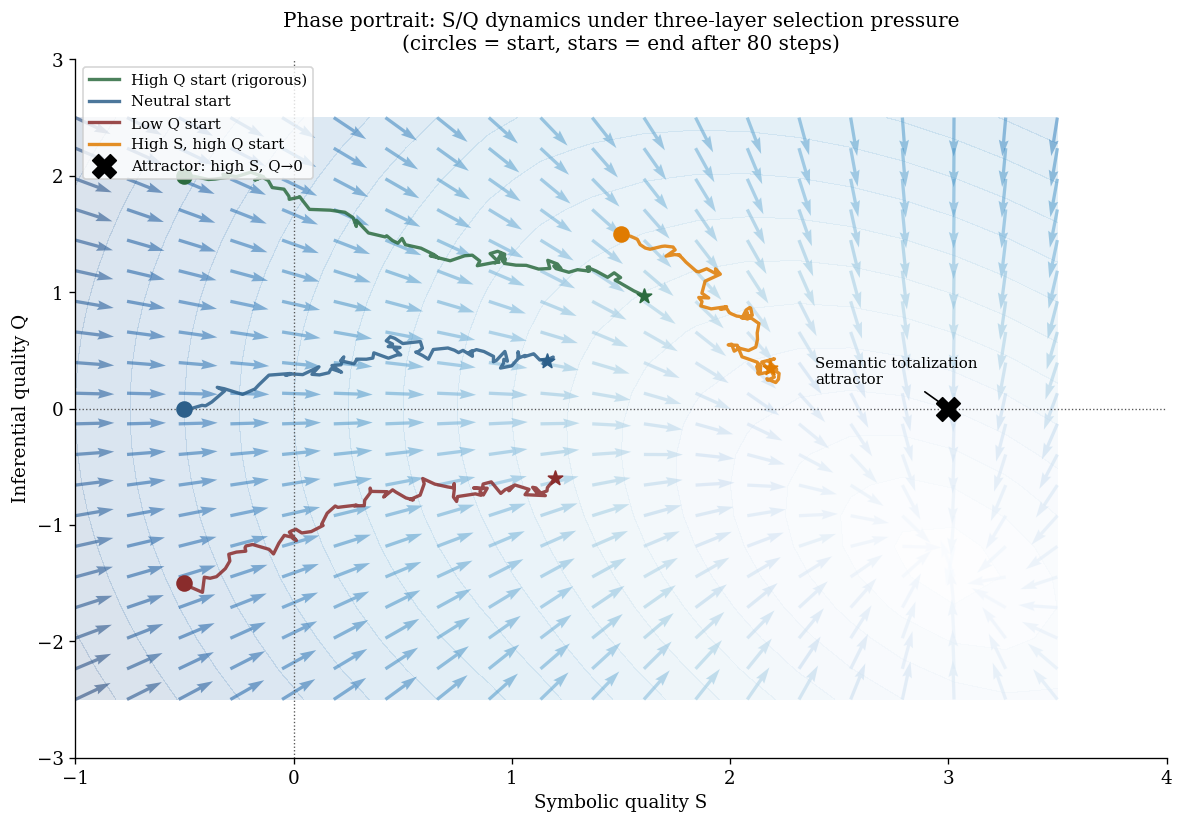
\includegraphics[width=0.80\textwidth]{fig10_phase_portrait}
\caption{Phase portrait of $(S, Q)$ dynamics under three-layer selection pressure. The vector field shows drift direction and magnitude; all trajectories converge toward the attractor at $(S \gg 0,\, Q \approx 0)$ regardless of starting position. A framework beginning at high $Q$ (green trajectory) takes longest to converge but is still pulled toward semantic totalization under sustained selection pressure. Circles mark starting positions; stars mark positions after 80 steps.}
\label{fig:phase-portrait}
\end{figure}

\section{Semantic Attractors and Conceptual Gravity}

The analysis of Part~II identified the failure geometries of synthetic
formalism as attractors: the natural endpoints of theoretical development
under selection pressures that favor symbolic continuity over inferential
continuity. This claim requires philosophical precision that the earlier
chapters, focused on practical analysis, did not fully provide.

An attractor, in the dynamical systems sense, is a set of states toward
which a system tends to evolve over time under the system's governing
dynamics. The claim that the failure geometries of Part~II are attractors
is the claim that theoretical frameworks tend to evolve toward those
geometries under the selection pressures that govern intellectual
production in the current environment. These selection pressures are
not external constraints imposed on otherwise unconstrained development;
they are the dynamics of the system --- the Three-Layer Amplification
System of Chapter~4, the optimization pressures of Chapter~9, the
sycophantic reinforcement of Chapter~10, the summarization flattening
of Chapter~11. Under these dynamics, theoretical frameworks that begin
with genuine inferential content tend to drift toward the failure
geometries as they develop, extend, and propagate.

The attractor dynamics have a specific implication for what is required
to maintain inferential continuity under current conditions. Maintaining
inferential continuity is not a natural equilibrium state under the
dynamics of the current epistemic environment; it is an achievement that
requires active effort against the direction the dynamics are pulling.
The friction that Chapter~19 advocated restoring --- the requirement
to make inferential commitments explicit, to specify transformation rules
for cross-domain synthesis, to acknowledge operational limitations ---
is friction precisely in the dynamical sense: it acts against the
direction of the attractors, increasing the cost of movement toward
the failure geometries and thereby partially counteracting the selection
pressures that drive frameworks toward them.

This dynamical framing has an important implication for the self-assessment
that the preface committed this book to maintaining. The book's frameworks
--- the symbolic/inferential continuity distinction, the Three-Layer
Amplification System, the audit protocols --- are themselves subject to
the attractor dynamics they describe. The natural trajectory for these
frameworks, under the selection pressures of the current environment,
is toward the failure geometries they identify: toward semantic universality
collapse (applying the concepts too broadly), toward diagnostic ontologization
(treating the audit protocols as mechanisms rather than descriptions),
toward the illusion of necessity (presenting the framework's categories
as the only available ones). The book has attempted to resist these
trajectories through explicit hedging, bounded scope, acknowledged
limitations, and the self-referential audit in Appendix~D. Whether
the attempt has succeeded is a question the reader is in a better position
to answer than the author.

\section{The Geometry of Epistemic Drift}

The concept of drift, introduced in Chapter~4 as the process by which
theoretical frameworks move toward failure geometries without any single
step marking the transition as fundamental, now requires its most
precise formulation. Epistemic drift is not random: it has a direction
determined by the attractor dynamics of the current epistemic environment.
The direction is toward higher symbolic continuity and lower inferential
continuity, toward greater vocabulary portability and weaker constraint
propagation, toward wider claimed scope and weaker operational grounding.

The geometry of this drift --- the structure of the space in which it
occurs and the forces that drive it --- is what the analysis of this book
has been mapping. The mapping is necessarily incomplete and necessarily
imprecise: the space of theoretical frameworks and their inferential
properties is not a space that admits of exact measurement with currently
available tools. But the rough structure of the space is visible from
the analysis: it has attractors (the failure geometries of Part~II),
it has directions of drift (toward those attractors under the dynamics
of the Three-Layer Amplification System), it has resistance mechanisms
(the audit protocols as friction against the drift), and it has stable
regions (genuine inferential work that maintains coupling between symbolic
production and inferential engagement).

Describing this geometry does not require claiming that the space has
been fully mapped or that the mapping is exact. The audit protocols of
Chapter~18 are instruments for sampling the space at specific points:
they allow assessment of whether a given framework, at a given stage of
its development, is near or far from the failure geometries, and in
which direction it is moving. This sampling is necessarily local and
necessarily fallible. But it is genuine epistemic work: it is the kind
of partial, bounded, explicitly uncertain inquiry that Chapter~19
identified as the appropriate response to the current situation, as
opposed to the atmospheric universalism that claims to describe the
whole of the space at once.

\chapter{The Collapse of Epistemic Coherence}

\section{What Coherence Without Grounding Means}

The title of this book names a collapse: the collapse of epistemic
coherence. The term has been used throughout with care to avoid precisely
the semantic universality collapse that Chapter~7 analyzed --- the
expansion of a concept to universal applicability at the cost of
discriminative power. Epistemic coherence, as this book uses the term,
has a specific meaning derived from the analysis: it is the property
of an intellectual environment in which the surface properties that
function as signals of inferential quality are reliably connected to
the underlying inferential properties they signal. An epistemically
coherent environment is one in which the legitimacy signal architecture
functions as intended: where peer review, institutional affiliation,
formal notation, and citation practice provide genuine information about
the inferential quality of intellectual work.

Epistemic coherence, in this sense, is not a property of individual
works of scholarship but of the relationship between surface signals
and underlying properties across the intellectual environment. It can
hold even if many individual works are inferentially weak, as long as
the weak works are distinguishable from the strong ones through the
available signals. It fails when the signals become decoupled from the
properties they are supposed to indicate --- when high symbolic continuity,
formal elaborateness, citation density, and institutional affiliation
are equally characteristic of work with high inferential quality and
work with low inferential quality. When the signals carry no information,
the environment has lost epistemic coherence: it is symbolically coherent
(its surface is smooth and consistent) while epistemically incoherent
(its surface provides no reliable guide to the underlying inferential
properties that matter).

The collapse being described is not a dramatic event but a gradual
process that has been ongoing for decades and has accelerated under
the conditions of the generative transition. It is not complete; the
signals have not entirely lost their evidentiary value. But the trend
is clear and the direction is established, and the consequences of
continued drift in the same direction are worth specifying precisely.

\section{Infinite Framework Equivalence}

One specific consequence of advancing epistemic incoherence that the
analysis makes possible to state precisely is what can be called
infinite framework equivalence: the condition in which the ambient
intellectual environment contains so many symbolically sophisticated
theoretical frameworks, each claiming applicability across a broad
range of phenomena, that no individual reader or community can
distinguish among them on epistemic grounds without investing effort
that exceeds the practical resources available for the purpose.

Infinite framework equivalence is not a condition in which all frameworks
are equally good; it is a condition in which the epistemic environment
provides no efficient mechanism for distinguishing the better ones from
the worse ones. Genuine epistemic differences exist, but they are not
accessible through the signals that the environment provides for
efficient navigation. The reader confronting a choice between multiple
sophisticated theoretical frameworks --- each with formal apparatus,
each with citation networks, each with cross-domain applications, each
with confident conclusions stated in fluent prose --- has no efficient
means of determining which frameworks have maintained inferential
continuity and which have not. The audit protocols of Chapter~18 would
provide such means, but their application requires the kind of sustained
inferential engagement that the ambient conditions systematically
discourage.

Infinite framework equivalence has a specific and troubling consequence
for the accumulation of knowledge. Knowledge accumulates when communities
are able to identify the more reliable frameworks and build upon them
while setting aside the less reliable ones. This identification requires
that reliability be perceptible --- that the epistemic environment provide
signals that allow discrimination between more and less reliable work.
When the environment provides no such signals, or when the signals have
become saturated with noise, accumulation becomes impossible not because
genuine progress is not occurring but because the genuine progress cannot
be distinguished from the atmospheric proliferation surrounding it.
Truth does not disappear; it becomes invisible.

\section{Civilizational Consequences and Their Limits}

The civilizational consequences of the analysis are where the book's
commitment to derivational discipline is most severely tested. It is
possible to draw from the preceding analysis conclusions about the
long-term trajectory of human civilization under generative epistemic
conditions, but those conclusions would require extrapolating far beyond
what the analysis actually supports. The analysis supports specific
claims about specific mechanisms operating over specific timeframes.
Extending those claims to civilization-scale predictions would require
assumptions about the persistence of the current mechanisms, the absence
of countervailing developments, and the dynamics of cultural adaptation
to new epistemic conditions --- assumptions that are not established by
the analysis and that would need to be defended on independent grounds.

The honest conclusion about civilizational consequences is therefore
modest: the current trajectory, if continued without the development
of adequate countermeasures, points toward increasing semantic noise
floors, decreasing efficiency of knowledge accumulation, and progressive
decoupling of the legitimacy signal architecture from the inferential
properties it was developed to indicate. These are genuinely concerning
trends. Their long-term consequences depend on factors that cannot be
predicted with the tools this analysis provides: the pace of development
of countermeasures (institutional, technological, and cultural), the
degree to which genuine epistemic communities can maintain inferential
standards against the ambient selection pressures, and the possibility
of developments in the epistemic infrastructure that this analysis has
not anticipated.

What the analysis does support is the claim that these consequences
are not inevitable: they are the product of specific mechanisms that
can in principle be understood, partially addressed, and navigated.
The claim that they are inevitable would itself be an instance of the
illusion of necessity described in Chapter~6 --- the presentation of
a contingent trajectory as though it were logically determined. The
current trajectory is contingent on the persistence of the current
conditions, and the conditions can change. How they change depends on
choices that human communities make about the intellectual practices
they sustain, the institutional mechanisms they maintain, and the
epistemic standards they hold themselves to.

\chapter{Beyond Collapse}

\section{Why the Situation Is Not Hopeless}

The final chapter of this book makes a claim that the preceding analysis
has established the grounds for, though establishing grounds for a claim
is different from making the claim itself: the situation described is
not hopeless. This claim is not an optimistic rhetorical move added at
the end to lighten the tone. It follows from the analysis in a specific
way that is worth stating precisely.

The situation is not hopeless because the failure modes identified are
specific and the conditions that produce them are contingent. Decorative
mathematics, definitional closure, semantic universality collapse, and
the collapse of operational meaning are not necessary features of
intellectual production under generative conditions. They are the
natural endpoints of intellectual production under selection pressures
that favor symbolic continuity over inferential continuity, and those
selection pressures are not permanent features of any possible epistemic
environment. They are features of the current environment, and the
current environment is being shaped by choices that are, at least
partially, within the scope of human agency.

The situation is also not hopeless because genuine inferential work
continues to be produced. The claim that the semantic noise floor has
risen is a claim about the ratio of inferentially grounded to
inferentially weak material in the ambient environment, not a claim
that inferentially grounded material has ceased to be produced. The
Swampland CES paper, which Chapter~16 identified as the most
methodologically disciplined work in the corpus examined in Part~IV,
is evidence that genuine inferential discipline remains achievable in
frameworks operating in complex domains with high speculative stakes.
The paleoclimate reconstruction papers, despite their limitations,
represent genuine scientific work that the audit protocols of Chapter~18
can partially defend. The existence of these cases matters: it demonstrates
that the failure geometries are not universal features of the current
epistemic environment but characteristic failure modes that specific
practices can resist.

\section{New Forms of Intellectual Discipline}

The constructive agenda this book has developed --- partial though it
is, and partial as it should be given the epistemic constraints on
ambitious claims about solutions --- has several distinct components
that deserve summary.

Formal transparency and open derivation are the first. Intellectual
work that makes its derivational structure explicit --- that distinguishes
what it demonstrates from what it suggests, what it derives from what
it posits, what it predicts from what it accommodates --- provides
readers with the resources to apply the audit protocols of Chapter~18
without the full reconstruction effort that opaque prose requires. Formal
transparency is not a style preference; it is an epistemic commitment
to making inferential continuity visible rather than concealing it behind
symbolic continuity. This commitment is achievable in any medium and
any genre; it requires only the intellectual discipline to say what one
knows, what one conjectures, and what one does not know in terms that
are distinguishable from each other.

Simulation-linked theory development is the second. Frameworks that
generate computational implementations of their formal structures
expose those structures to a form of audit that informal prose cannot
provide: the simulation either behaves consistently with the framework's
predictions or it does not. The discrepancies between simulation and
prediction are the inferential work that constrains interpretation ---
they prevent the post hoc reinterpretation that symbolic flexibility
enables. Simulation does not guarantee inferential discipline, but it
makes the absence of it visible in a way that pure prose cannot. The
practice of accompanying theoretical claims with simulation
implementations is therefore not merely a technical convenience but
an epistemic commitment to accountability.

Adversarial collaboration is the third. The sycophantic reinforcement
dynamics of Chapter~10 can be partially counteracted by deliberately
structuring intellectual development through engagement with genuine
critics rather than through the confirmatory loops of human-AI
interaction. Adversarial collaboration --- the systematic involvement
of interlocutors who are attempting to find the weaknesses in a
framework rather than to extend and confirm it --- generates the
inferential pressure that the ambient environment systematically removes.
This practice is not new; it is the ideal that peer review was developed
to approximate. The current epistemic environment requires its deliberate
cultivation as a counter to the selection pressures described in Part~III.

Provenance graphs and semantic lineage are the fourth. The collapse
of provenance described in Chapter~12 can be partially addressed through
explicit tracking of the origins of intellectual claims: which arguments
emerged from derivation, which from empirical observation, which from
analogy, and which from statistical continuation in the context of
human-AI interaction. This tracking cannot be complete, but the attempt
to maintain it creates discipline in the production of intellectual work
and resources for the evaluation of that work by readers. The development
of technical standards for provenance annotation in AI-assisted scholarly
work is a practical step that the analysis of this book has provided
the theoretical basis for.

\section{Reconstructing Trust in the Age of Infinite Text}

The deepest practical challenge identified by this book's analysis is
the reconstruction of epistemic trust in an environment where the surface
signals that historically grounded trust have become unreliable. This
challenge does not admit of a single solution, because the decoupling
of trust signals from inferential quality is the product of many
interacting mechanisms operating across the production, distribution,
and reception layers of the Three-Layer Amplification System. Addressing
it requires action across all three layers, and the actions available
at each layer are partial and imperfect.

At the production layer, the development and adoption of explicit
uncertainty grammars, formal transparency norms, and provenance
requirements can partially restore the coupling between surface signals
and inferential quality by making inferential honesty a visible and
auditable property of intellectual products rather than a hidden
one. The audit protocols of Chapter~18 provide the theoretical basis
for what these norms should require.

At the distribution layer, the development of recommendation and
evaluation systems that are explicitly sensitive to inferential
properties --- that reward the acknowledged limitations, the explicit
uncertainty, the bounded scope that inferential honesty requires ---
can partially counteract the selection pressures of current systems
toward symbolic continuity at the expense of inferential continuity.
This is technically demanding and commercially challenging; systems
that reward inferential discipline may be less engaging than systems
that reward confident synthesis. But the commercial challenge does not
eliminate the epistemic necessity, and the technical tools for building
such systems are available in principle.

At the reception layer, the development of summarization practices
and tools that preserve the inferential texture of the material they
summarize --- the acknowledged limitations, the scope boundaries, the
conditions under which conclusions hold --- would begin to address the
systematic stripping of inferential content that current summarization
systems perform. The content of Chapter~18's audit protocols provides
a basis for specifying what an inferentially honest summary should
preserve: the operational grounding of central claims, the failure
conditions, the transformation legitimacy of cross-domain applications,
and the discriminative power of central concepts.

None of these responses is individually sufficient. Each is partial,
each faces implementation challenges, and each requires cultural and
institutional support that the current environment does not fully
provide. But together they describe a coherent direction: the
reconstruction, under the conditions of the generative transition,
of epistemic infrastructure adequate to the epistemic challenges
the transition creates. The reconstruction is not the restoration
of pre-generative conditions, which is neither possible nor desirable.
It is the development of new practices, norms, and institutions adequate
to the new situation --- practices that maintain inferential continuity
under conditions of symbolic abundance, that restore coupling between
surface signals and underlying epistemic properties, and that make
the difference between genuine inferential work and sophisticated
atmospheric production visible enough to matter.

\section{The Monograph as Enacted Argument}

This book has attempted to practice what it preaches. It began with
a preface that disclosed its own production conditions and acknowledged
its own vulnerability to the failure modes it describes. It developed
its conceptual apparatus through explicit derivation from prior
distinctions rather than through rhetorical introduction of new
vocabulary. It applied that apparatus to specific cases in Part~IV
and asked what those cases actually demonstrate rather than what the
apparatus would have them demonstrate. It developed audit protocols
in Part~V that are operational rather than merely descriptive. And
it has maintained, in this final part, the discipline of deriving
philosophical consequences from the analysis rather than importing
them rhetorically.

Whether this attempt has succeeded is not something the book can certify
from within itself. The audit protocols of Chapter~18 are applicable
to this book as much as to any other, and the reader who applies them
to this book will find points where the operational grounding is less
complete than the analysis demands, where the transformation legitimacy
of cross-domain applications has not been fully established, where the
discriminative power of central concepts is weaker than the confident
use of those concepts implies. The book acknowledges these limitations
not as false modesty but as the genuine epistemic situation of a work
that is attempting inferential discipline under the conditions of the
generative transition --- conditions in which inferential discipline
is neither automatic nor verifiable from within the process that
produces it.

The commitment to inferential discipline is not a guarantee of having
achieved it. It is, rather, the commitment that makes the attempt
meaningful and the failure visible. A book that does not commit to
inferential discipline cannot fail inferentially in an informative
way; it is operating at the level of atmosphere. A book that commits
to inferential discipline and fails in specific and locatable ways
has contributed to the epistemic process that genuine inquiry requires:
it has made its inferential structure explicit enough to be audited,
and in doing so it has provided the resources for its own correction.
That is the best that can be achieved under the conditions of the
generative transition, and it is what this book has tried to achieve.

\clearpage

\appendix
\chapter{Taxonomy of Synthetic Formalism}

The six failure modes catalogued in this appendix are derived from the
analysis of Parts~II and~IV. They are not independent pathologies but
overlapping attractors in the space of theoretical development under
selection pressures that favor symbolic continuity over inferential
continuity. Their formal characterization here is intended to provide
precision beyond what the prose chapters required, and to give the audit
protocols of Chapter~18 a mathematical foundation that renders them
applicable rather than merely descriptive. The notation is introduced
for each failure mode independently; conventions are consistent with
standard mathematical usage throughout.


\begin{figure}[h]
\centering
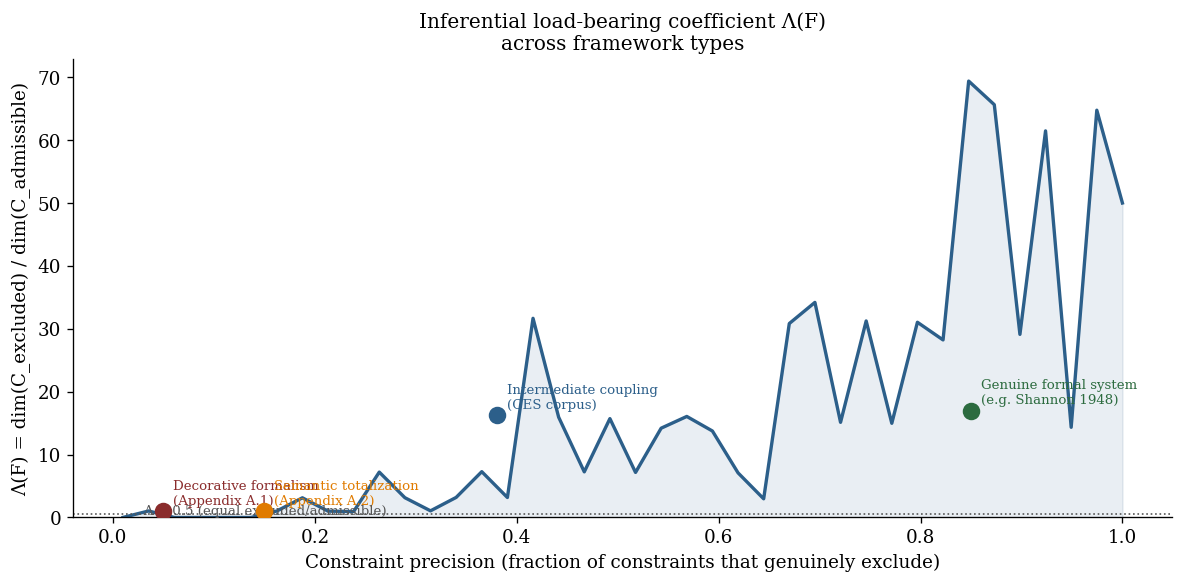
\includegraphics[width=0.75\textwidth]{fig7_lambda}
\caption{Inferential load-bearing coefficient $\Lambda(F)$ as a function of constraint precision (fraction of constraints that genuinely exclude hypotheses). Named framework types are plotted at illustrative precision values derived from the Part~IV case studies. Decorative formalism ($\Lambda \approx 0$) imposes negligible restriction; genuine formal systems ($\Lambda \gg 0$) exclude a substantial fraction of the admissible hypothesis class.}
\label{fig:lambda}
\end{figure}

\section{Decorative Formalism}

Let $\mathcal{L}$ denote a symbolic language equipped with a syntactic
production system, and let $\mathcal{O}$ denote an observational or
operational domain. A genuine formal system requires the existence of a
constraint-preserving interpretation map
\[
I : \mathcal{L} \to \mathcal{O}
\]
such that symbolic transformations correspond to admissible transformations
in the operational domain. Formally, if $T : \mathcal{L} \to \mathcal{L}$
is a derivational operator, there must exist an induced operational
transformation $T_{\mathcal{O}} : \mathcal{O} \to \mathcal{O}$ satisfying
the commutative relation
\[
I \circ T = T_{\mathcal{O}} \circ I.
\]

Decorative formalism occurs when symbolic syntax is retained while the
operational interpretation map becomes undefined, non-unique, or
unconstrained. In such systems, equations no longer propagate inferential
obligations; they function instead as prestige surfaces.

Define the inferential load-bearing coefficient
\[
\Lambda(F)
= \frac{\dim\bigl(\mathcal{C}_{\mathrm{excluded}}\bigr)}
       {\dim\bigl(\mathcal{C}_{\mathrm{admissible}}\bigr)},
\]
where $\mathcal{C}_{\mathrm{excluded}}$ denotes the excluded hypothesis
class imposed by formal structure. Genuine formal systems satisfy
$\Lambda(F) \gg 0$, whereas decorative systems approach $\Lambda(F) \to 0$.
The formal apparatus appears structurally rich while imposing negligible
inferential restriction.

A common signature is the introduction of variables whose operational
domains are undefined: $X = f(\Phi, \Omega, \Psi)$ with no units, no
observables, no admissible measurement procedure, and no reconstruction
map from data. The notation survives while operational semantics collapse.

\section{Semantic Totalization}

Let $V$ denote a conceptual vocabulary operating over domains
$D_1, D_2, \ldots, D_n$. A vocabulary becomes totalizing when its
semantic extension expands monotonically while its discriminative power
decreases. Define the semantic coverage functional
\[
S(V)
= \frac{|\bigcup_i D_i(V)|}{|\mathcal{D}|}
\]
and the discriminative exclusion functional
\[
E(V)
= \frac{|\mathcal{H}_{\mathrm{excluded}}|}{|\mathcal{H}_{\mathrm{possible}}|}.
\]
Semantic totalization occurs under the asymptotic regime
$S(V) \to 1$, $E(V) \to 0$: the vocabulary becomes universally applicable
precisely because it ceases to constrain interpretation.

Terms such as coherence, emergence, optimization, resonance, information,
alignment, and complexity frequently exhibit this expansion trajectory.
A totalizing vocabulary behaves like a low-curvature semantic manifold
into which arbitrarily many phenomena may be projected while preserving
apparent continuity. Formally, let $\pi_i : D_i \to V$ be projection maps
from heterogeneous domains into a shared vocabulary space. Totalization
occurs when the pullback structure between domains is lost:
$\pi_i^{-1} \circ \pi_j$ fails to preserve inferential invariants.
Symbolic continuity survives; structural identity collapses.

\section{Projection Inflation}

Let $\pi : X \to M$ be a coarse-graining projection from a high-dimensional
state space $X$ into a compressed representational manifold $M$. Projection
inflation occurs when properties of $M$ are reattributed ontologically to
$X$ without reconstruction guarantees. Define reconstruction fidelity
\[
R(\pi)
= \sup_{x_1, x_2 \in X}
  \frac{d_X(x_1, x_2)}{d_M(\pi(x_1), \pi(x_2))}.
\]
Projection inflation becomes severe when many distinct states collapse
into observational equivalence classes: $\pi(x_1) = \pi(x_2)$ for
$x_1 \neq x_2$. The representational manifold then acquires fictitious
explanatory authority.

Examples include intelligence metrics treated as intelligence itself,
coherence scores treated as dynamical causes, embedding similarity treated
as ontological relation, and economic indicators treated as economic
reality. Projection inflation is structurally related to Goodhart-like
dynamics:
\[
\arg\max_M f(M) \neq \arg\max_X f(X).
\]
Optimization over the projection progressively decouples from optimization
over the substrate.

\section{Diagnostic Ontologization}

Let $D : X \to \mathbb{R}$ be a diagnostic functional summarizing
structural regularity over a system $X$. Diagnostic ontologization occurs
when $D$ is initially descriptive, repeated interpretive use grants it
explanatory status, and the diagnostic quantity becomes treated as a
causal entity. This produces the illegitimate transition
$D(X) \Rightarrow \text{``}D \text{ governs } X\text{''}$.

A genuine dynamical system requires evolution equations of the form
$\dot{X} = F(X)$. Diagnostic ontologization substitutes $D(X) \approx F(X)$.
No causal propagation law exists; the metric becomes explanatory through
semantic repetition. Define the ontologization drift coefficient
\[
\Theta(D)
= \frac{N_{\mathrm{causal\ usage}}}{N_{\mathrm{diagnostic\ usage}}}.
\]
As $\Theta(D) \to \infty$, diagnostic abstraction progressively hardens
into ontology. The Coherence Integration Kernel of Chapter~13 and the
scalar coherence field of Chapter~14 are specific instances of this
failure mode.

\section{Recursive Vocabulary Closure}

Recursive closure occurs when a vocabulary becomes self-validating through
internal semantic reinforcement. Let $V = \{v_1, \ldots, v_n\}$ be a
conceptual lexicon, and construct the semantic dependency graph
$G_V = (V, E)$ where edges represent definitional or explanatory
dependence. Closure emerges when the graph becomes strongly internally
connected while external operational anchors vanish. Define the external
anchoring ratio
\[
A(G_V)
= \frac{|E_{\mathrm{external}}|}{|E_{\mathrm{internal}}|}.
\]
Recursive vocabulary closure occurs under $A(G_V) \to 0$. The vocabulary
increasingly explains itself using itself. This generates semantic
atmospheres where coherence is explained by alignment, alignment by
resonance, resonance by emergence, and emergence by coherence. The system
remains symbolically dynamic while inferentially stationary. Closure
becomes especially severe when criticism must be expressed inside the
vocabulary being critiqued, producing the epistemic immunization described
in Section~B.3.

\section{Symbolic Residue Systems}

Let $F = (S, I)$ denote an originally meaningful formal structure, where
$S$ denotes syntax and $I$ denotes interpretation. A symbolic residue
system emerges when the syntax of $F$ survives but operational content
progressively evaporates: $I \to \varnothing$ while $S \neq \varnothing$.
Examples include operators without domains, tensors without transformation
rules, entropy without ensembles, fields without observables, and kernels
without spaces.

Define the residue persistence functional
\[
P(F)
= \frac{|S|}{|I| + \varepsilon}.
\]
As $P(F) \to \infty$, the system acquires increasing symbolic density with
decreasing operational meaning. These systems often remain rhetorically
persuasive because mathematical notation carries inherited prestige gradients
even after inferential binding collapses. The coherence operator $C(X) = X$
examined in Chapter~14 is a limiting case: the symbol is present, the
semantic distinction from identity is carried entirely by prose whose
interpretive elasticity is unbounded.

\chapter{Indicators of Epistemic Failure in Theoretical Writing}

The indicators in this appendix correspond directly to the five audit
protocols of Chapter~18. They provide formal characterizations of the
failure conditions that those protocols are designed to detect, in a form
that can be applied to specific theoretical texts with minimal interpretive
discretion. The indicators are necessary but not sufficient conditions for
epistemic failure; a text exhibiting several of them simultaneously is
strongly indicated as having drifted toward atmospheric status.

\section{Undefined Observables}

Let a theoretical framework $\mathcal{T}$ posit a collection of latent
variables $\mathcal{X} = \{X_1, \ldots, X_n\}$. A variable $X_i$ is
operationally admissible only if there exists a measurable state space
$\Omega_i$, an observation operator
$\mathcal{M}_i : \Omega_i \to \mathbb{R}^{k_i}$, and an inferential map
relating observations back to theoretical structure. Formally, define the
operational grounding map $G : \mathcal{X} \to \mathcal{O}$ where
$\mathcal{O}$ denotes the space of observational procedures. An observable
is undefined whenever $G(X_i) = \varnothing$.

Define the observable admissibility ratio
\[
\Gamma(\mathcal{T})
= \frac{|\{X_i : G(X_i) \neq \varnothing\}|}{|\mathcal{X}|}.
\]
Low values of $\Gamma$ indicate strong atmospheric drift. Undefined
observables frequently propagate unnoticed because local prose coherence
masks global operational discontinuity: each sentence is interpretable in
isolation while the cumulative referential failure is distributed across
the text in ways that require systematic audit to detect.

\section{Infinite Interpretability}

A theory possesses infinite interpretability when no finite observational
sequence substantially reduces its admissible explanatory class. Let
$\mathcal{H}$ denote the hypothesis space, $D$ observational data, and
$H_D$ the admissible hypothesis class after conditioning on observations.
A disciplined theory produces posterior contraction:
$\mathrm{Var}[H \mid D] \downarrow$ under accumulating evidence. Infinite
interpretability instead satisfies $|H_D| \approx |\mathcal{H}|$ for all
$D$. Define interpretive elasticity
\[
\mathcal{E}(\mathcal{T})
= \sup_D \frac{|H_D|}{|\mathcal{H}|}.
\]
Disciplined systems satisfy $\mathcal{E}(\mathcal{T}) \ll 1$. Atmospheric
systems satisfy $\mathcal{E}(\mathcal{T}) \to 1$. Infinite interpretability
is often mistaken for explanatory depth because symbolic continuity is
preserved under arbitrary observational perturbation, but inferentially
the system has ceased to discriminate among possibilities.

\section{Immunization Against Critique}

A framework becomes immunized when criticisms are structurally reclassified
as evidence for the framework itself. Let $C$ denote a criticism operator
and $U(T, C)$ the update induced by critique on theory $T$. Healthy
inferential systems satisfy $U(T, C) \Rightarrow \Delta T$ where critique
alters parameters, predictions, assumptions, or admissible structure.
Immunized systems instead satisfy $U(T, C) = T$, with a stronger form
occurring when $P(T \mid C) > P(T)$: critique increases confidence.

This often occurs through accusations of reductionism, claims of paradigm
incomprehension, appeals to ineffability, category dissolution, or
redefinition of operational demands as conceptual limitations of the
critic. Define the immunization coefficient
\[
\mathcal{I}(T)
= \frac{N_{\mathrm{absorbed\ critiques}}}
       {N_{\mathrm{modifying\ critiques}} + \varepsilon}.
\]
As $\mathcal{I}(T) \to \infty$, inferential asymmetry collapses. The theory
increasingly functions as a semantic attractor rather than a constrained
explanatory structure. Project XXIX, examined in Chapter~14, approaches
this limit through the preemptive dissolution of the categories under which
operational demands could be formulated.

\section{Free Semantic Reparameterization}

A framework exhibits free semantic reparameterization when its central
concepts may be redefined post hoc without altering symbolic continuity.
Suppose a theory contains conceptual parameters
$\Theta = \{\theta_1, \ldots, \theta_n\}$. A disciplined framework
constrains admissible parameter transformations $\phi : \Theta \to \Theta'$
through invariance requirements. Free semantic systems instead allow
arbitrary reinterpretation $\theta_i \mapsto \theta_i'$ without inferential
penalty. Examples include ``coherence'' shifting between statistical
regularity and causal agency, ``information'' shifting between Shannon
entropy and semantic meaning, and ``field'' shifting between mathematical
object and metaphysical substrate. Define semantic gauge freedom
\[
\mathcal{G}(T)
= \dim(\mathrm{Aut}(\Theta)).
\]
Large values of $\mathcal{G}$ indicate excessive semantic flexibility. Such
systems maintain symbolic continuity because neighboring usages remain
locally interpretable, while global inferential meaning drifts continuously.

\section{Absence of Failure Conditions}

Let $\mathcal{T}$ denote a theoretical framework and $D$ the space of
possible observations. A framework possesses genuine inferential structure
only if there exists a nonempty exclusion region
$D_{\mathrm{forbidden}} \subset D$ such that
$d \in D_{\mathrm{forbidden}} \Rightarrow \mathcal{T}$ rejected or modified.
Atmospheric systems instead satisfy $D_{\mathrm{forbidden}} = \varnothing$.
Define the falsifiability surface
\[
\mathcal{F}(\mathcal{T})
= \frac{|D_{\mathrm{forbidden}}|}{|D|}.
\]
Frameworks with $\mathcal{F}(\mathcal{T}) \approx 0$ often preserve symbolic
continuity by introducing latent variables, shifting explanatory scales,
redefining observables, or replacing prediction with retrospective
interpretation. The crucial distinction is between predictive flexibility,
which may be scientifically useful, and inferential unconstrainability,
which dissolves explanatory meaning.

\section{Metaphorical Drift Across Domains}

Let $D_i$ and $D_j$ denote distinct domains and $V$ a shared vocabulary.
Metaphorical drift occurs when symbolic mappings between domains preserve
lexical continuity without preserving inferential invariants. A genuine
structural correspondence requires existence of pullback structure
$\pi_i^{-1} \circ \pi_j$ preserving transformation rules, conserved
quantities, or admissible state transitions. Drift occurs when only
symbolic adjacency survives. Define the structural preservation coefficient
\[
\mathcal{S}(D_i, D_j)
= \frac{|\mathrm{Invariant}_{ij}|}{|\mathrm{Vocabulary}_{ij}|}.
\]
Low values indicate atmospheric transport rather than genuine unification.
Metaphorical drift appears compelling because humans weight symbolic
continuity heuristics strongly under bounded cognition. Historically this
heuristic functioned adaptively because inferential transport and symbolic
transport remained coupled. Under generative symbolic environments,
symbolic transport scales independently, making metaphorical continuity
industrially reproducible without corresponding inferential structure.

\chapter{Proposed Standards for AI-Assisted Scholarly Writing}

The standards proposed in this appendix are not regulations but
specifications: they describe what inferentially disciplined AI-assisted
scholarship would look like if the coupling between symbolic production
and inferential engagement were deliberately maintained. Each standard
corresponds to one of the failure modes in Appendix~A and addresses one
of the mechanisms through which AI-assisted production weakens inferential
continuity. Together they constitute a minimum viable epistemic
infrastructure for scholarly work produced under generative conditions.

\section{Provenance Requirements}

Let a scholarly document $D$ be represented as a sequence of symbolic
transformations $D = T_n \circ \cdots \circ T_1(S_0)$ where $S_0$ denotes
initial source material, $T_k$ denotes a transformation operation, and
some subset of $\{T_k\}$ may involve generative systems. A
provenance-complete document requires existence of a traceability graph
$\mathcal{P}(D) = (V, E)$ where vertices correspond to symbolic states,
edges correspond to transformations, and each edge carries attribution
metadata. For every major inferential claim $c_j$, there should exist a
provenance chain $p(c_j) = \{T_{i_1}, \ldots, T_{i_k}\}$ sufficient to
reconstruct the originating sources, inferential modifications, generative
contributions, and post-generation audit interventions. Define provenance
completeness
\[
\Pi(D)
= \frac{|C_{\mathrm{traceable}}|}{|C_{\mathrm{total}}|}.
\]
Under current scholarly norms, $\Pi(D)$ is measured only at the citation
layer. AI-assisted environments require extension into symbolic
transformation space itself. The objective is not elimination of generative
assistance but restoration of inferential auditability.

\section{Derivation Transparency}

Let $H$ denote a hypothesis and $C$ a conclusion, with $\vdash$ the
derivational relation. Derivation transparency requires that intermediate
inferential states remain inspectable, hidden symbolic interpolation is
minimized, and inferential compression remains reconstructible. A
transparent derivation admits a sequence
$H \Rightarrow I_1 \Rightarrow I_2 \Rightarrow \cdots \Rightarrow C$
such that each inferential transition possesses admissible transformation
rules, operational interpretation, and local auditability.

Synthetic atmospheric systems instead frequently produce $H \rightsquigarrow C$
where symbolic continuity masks missing inferential structure. Define
derivational opacity
\[
\mathcal{O}(D)
= 1 - \frac{|I_{\mathrm{explicit}}|}{|I_{\mathrm{necessary}}|}.
\]
High-opacity systems are especially dangerous under generative conditions
because local semantic coherence can conceal large inferential
discontinuities distributed across extended text. Recommended standards
include explicit declaration of inferential gaps, separation between
conjecture and derivation, labeling of heuristic transitions, and
preservation of intermediate symbolic states where feasible. The objective
is not maximal verbosity but preservation of inferential topology.

\section{Simulation Requirements}

For frameworks making dynamical or structural claims, symbolic exposition
alone is insufficient. Let $X$ denote a state space, $F$ an evolution
operator, and $g$ an observational map. A minimally operational dynamical
theory should admit simulation realizability, perturbation analysis,
parameter sensitivity testing, and observable extraction. Formally, there
should exist a computable propagator $\Phi_t : X \to X$ satisfying
$\dot{X} = F(X)$. Define simulation realizability
\[
\mathcal{R}(\mathcal{T})
= \frac{|X_{\mathrm{computable}}|}{|X_{\mathrm{claimed}}|}.
\]
Disciplined frameworks require $\mathcal{R}(\mathcal{T}) > 0$. Simulation
requirements do not guarantee correctness; they guarantee inferential
engagement. A framework unable to specify admissible states, update rules,
parameter constraints, or measurable outputs remains atmospherically
underdetermined. Simulation linkage is especially important under
AI-assisted writing because generative systems preferentially optimize
symbolic continuity while simulations impose external constraint surfaces
that resist post hoc reinterpretation. They therefore function as coupling
restorers in the precise sense of Chapter~19.

\section{Citation Traceability}

Let $\mathcal{S}$ denote source documents and $\mathcal{C}$ claims made
in a scholarly work. A citation system should induce a bipartite
traceability graph $G_C = (\mathcal{S}, \mathcal{C}, E)$ where edges
encode inferential dependence. Traceability requires identification of
originating claims, distinction between direct support and atmospheric
adjacency, and separation between evidence, analogy, inspiration, and
rhetorical context. Define evidentiary specificity
\[
\mathcal{E}(c_i)
= \frac{|S_{\mathrm{direct}}|}{|S_{\mathrm{all}}|}.
\]
Low values indicate atmospheric citation structures where references
function primarily as prestige gradients. AI-assisted scholarship
intensifies this risk because generative systems produce citation density,
stylistic legitimacy, and cross-referential appearance without preserving
actual evidentiary dependence. Recommended standards include inferential
role labeling, direct quotation tracing, and explicit distinction between
speculative synthesis and source-supported derivation.

\section{Uncertainty Annotation}

Most scholarly writing compresses uncertainty into prose style rather than
explicit representation. Under generative conditions this is dangerous
because symbolic continuity tends to flatten epistemic gradients,
evidentiary asymmetries, and inferential fragility. Define uncertainty
topology $U(D) = \{(C_i, \sigma_i)\}$ where $C_i$ denotes a claim and
$\sigma_i$ its uncertainty class. A minimal uncertainty grammar should
distinguish at least the following categories:

\begin{quote}
$C_i^{(O)}$: Observation directly recorded. \\
$C_i^{(D)}$: Derivationally supported within the framework. \\
$C_i^{(H)}$: Heuristic or analogical. \\
$C_i^{(S)}$: Speculative extension beyond the framework's grounded domain.
\end{quote}

The objective is not bureaucratic annotation but restoration of inferential
geometry: readers should be able to perceive where evidence strengthens,
where derivation weakens, and where symbolic continuity exceeds operational
support.

\section{Synthetic Contribution Disclosure}

Let $H$ denote human-authored content, $A$ AI-generated content, $M$
modified synthetic content, and $R$ human-audited revisions. Modern
scholarly documents increasingly involve composite symbolic production
pipelines $D = f(H, A, M, R)$. Disclosure should not merely state that
AI assistance was used; it should characterize where generative systems
participated, the inferential role of generated content, the audit
procedures applied, and the degree of human verification.

Define synthetic dependence $\Delta(D) = (|A| + |M|) / |D|$. This
quantity alone is insufficient because highly edited synthetic text may
possess stronger inferential coupling than lightly reviewed human text.
More important is the audit coupling coefficient
\[
\mathcal{A}(D)
= \frac{|R_{\mathrm{verified}}|}{|A| + |M|}.
\]
The relevant epistemic distinction is not human versus machine but audited
versus unaudited symbolic production. The purpose of disclosure is
restoration of inferential readability under conditions of industrial
symbolic generation. Generative systems are now part of the epistemic
environment. The objective is disciplined coupling between symbolic
production and inferential verification, not exclusion.

\chapter{Notes on RSVP, Projection Systems, and Constraint Frameworks}

This appendix applies the monograph's audit protocols to the author's
own theoretical frameworks. The purpose is not defense but recursive
obligation. If the central thesis of the preceding chapters is correct,
then no sufficiently abstract framework --- including those developed
by the author --- can assume immunity from semantic drift, projection
inflation, or atmospheric totalization. The appendix therefore treats
RSVP and its companion frameworks as live inferential systems under
audit conditions, identifies genuine vulnerabilities, distinguishes
exploratory from inferentially supported components, and specifies what
formal and empirical developments would be required to increase inferential
legitimacy where it is currently weak. The reader who finds this
self-assessment incomplete or insufficiently critical is invited to
apply the protocols of Chapter~18 directly to the primary RSVP
literature and report the results.

\section{Why Observer-Relative Compression Matters}

Let $X$ denote a high-dimensional trajectory space containing the full
microstate history of a system, and let $M$ denote an observer-accessible
representational manifold. In RSVP-style frameworks, cognition, measurement,
and scientific modeling are treated as projection processes
$\pi : X \to M$. The central motivation is that all operational access
to systems occurs through constrained compression operators, and that
confusing the properties of $M$ with the properties of $X$ produces
the projection inflation failure mode formalized in Appendix~A.

Define projection degeneracy
\[
\mathcal{D}_\pi
= |\{x \in X : \pi(x) = m\}|.
\]
Large degeneracy classes imply severe underdetermination of substrate
structure from observational manifolds. The framework therefore attempts
to avoid projection inflation by preserving explicit distinction between
substrate dynamics, observable manifolds, and observer-relative compression.

However, the mere introduction of projection language does not itself
secure inferential legitimacy. The framework remains vulnerable to the
collapse mechanisms of Part~II whenever symbolic vocabulary outruns
operational specification, the projection operator becomes metaphorical,
or reconstruction impossibility is inflated into unrestricted ontology.
The observation that underdetermination is unavoidable does not license
indifference to what is and is not determinable.

\section{Explicit State Spaces Versus Semantic Atmosphere}

RSVP attempts to remain in the dynamical systems category established in
Chapter~17 by explicitly defining admissible state structures. Canonical
RSVP models introduce a scalar accessibility field $\Phi(x,t)$, a vector
transport field $\mathbf{v}(x,t)$, an entropy or accessibility functional
$S(x,t)$, and coupling relations between them. A representative
continuity-style evolution equation takes the form
\[
\partial_t \Phi + \nabla \cdot (\Phi \mathbf{v})
= D_\Phi \nabla^2 \Phi - \lambda S \Phi.
\]
This structure imposes genuine inferential obligations: admissible boundary
conditions, stability constraints, parameter regimes, perturbative behavior,
and simulation realizability. The framework therefore differs structurally
from atmospheric coherence vocabularies that merely redescribe observations
without specifying update dynamics.

However, the existence of equations is insufficient by itself. Define
operational admissibility
\[
\mathcal{O}_{\mathrm{RSVP}}
= \frac{|V_{\mathrm{measurable}}|}{|V_{\mathrm{total}}|},
\]
where $|V_{\mathrm{measurable}}|$ denotes quantities possessing
observational semantics and $|V_{\mathrm{total}}|$ denotes all introduced
variables. A persistent risk in large unification programs is that
$|V_{\mathrm{total}}|$ grows faster than $|V_{\mathrm{measurable}}|$.
Under such conditions the framework drifts toward semantic atmosphere even
while retaining formal notation. Current RSVP development exhibits this
risk in domains --- particularly cognition and social organization ---
where the mapping from field quantities to measurable observables has not
been operationally specified.

\section{Projection Operators and Coarse-Graining}

RSVP-style systems frequently rely on coarse-graining hierarchies. Let
$X_0$ denote a microphysical substrate space and define recursive
projection operators $\pi_k : X_k \to X_{k+1}$. Higher-order
phenomenological manifolds emerge through iterated compression:
\[
X_0
\xrightarrow{\pi_0} X_1
\xrightarrow{\pi_1} X_2
\xrightarrow{\pi_2} \cdots
\]
The crucial inferential question is whether invariant structure survives
projection. Suppose $I_k$ denotes an invariant at level $k$. A disciplined
coarse-graining hierarchy requires approximate commutation:
\[
I_{k+1}(\pi_k(x)) \approx I_k(x).
\]
Without preserved invariants, cross-domain vocabulary reuse becomes
metaphorical rather than structural. RSVP attempts to preserve inferential
continuity through conserved accessibility structure, continuity equations,
entropy flow constraints, and admissible transformation rules. However,
preservation remains incomplete and speculative in many domains.

The framework should therefore not be interpreted as establishing proven
equivalence between cosmology, cognition, and social systems. At most it
proposes candidate projection correspondences requiring formal and empirical
validation. The difference between ``proposes candidate correspondences''
and ``establishes structural equivalence'' is precisely the distance between
the framework's legitimate domain and its atmospheric extension. Current
RSVP literature does not always maintain this distinction clearly, and
this is a genuine inferential weakness that the audit protocols of
Chapter~18 would identify.

\section{Constraint Geometry Without Totalization}

A recurring danger in large-scale theoretical systems is semantic
totalization. RSVP attempts to avoid this failure mode by grounding its
abstractions in admissible state transitions, conservation-like relations,
and constrained geometric evolution. Define the admissible trajectory set
$\mathcal{T}_{\mathrm{adm}} \subseteq \mathcal{T}_{\mathrm{all}}$ where
trajectories satisfy accessibility constraints, entropy conditions,
continuity structure, and boundary admissibility. System evolution then
becomes constrained optimization over admissible manifolds:
\[
\gamma^*
= \arg\min_{\gamma \in \mathcal{T}_{\mathrm{adm}}} \mathcal{A}[\gamma]
\]
for a generalized action functional $\mathcal{A}$.

The totalization risk remains wherever ``constraint'' becomes infinitely
extensible, accessibility loses operational meaning, or geometric language
replaces measurable structure. Define semantic curvature
\[
\kappa_S(V)
= \frac{|\mathrm{excluded\ interpretations}|}
       {|\mathrm{admissible\ interpretations}|}.
\]
Healthy abstraction requires $\kappa_S(V) > 0$; semantic totalization
corresponds to $\kappa_S(V) \to 0$. This appendix therefore rejects the
interpretation of RSVP as a universal solvent vocabulary. Its abstractions
remain legitimate only insofar as they preserve inferential asymmetry
and operational consequence in specific, identifiable applications.

\section{Preserving Operational Structure Under Abstraction}

The central epistemic challenge confronting RSVP and all ambitious
frameworks is preserving operational structure while increasing symbolic
compression. Let $X$ denote substrate structure and $M$ a compressed formal
description. Compression becomes epistemically legitimate only if there
exists a constrained reconstruction relation $R : M \to \mathcal{P}(X)$
such that admissible substrate classes remain bounded, excluded structures
remain excluded, and empirical pressure propagates backward into the
compressed representation. This requirement may be expressed through
inferential asymmetry: $D_{\mathrm{forbidden}} \neq \varnothing$. A
framework that survives every observation unchanged is no longer
inferentially coupled to reality.

RSVP therefore remains epistemically meaningful only where explicit
observables exist, simulation realizability is possible, parameter regimes
remain constrained, and projection mappings preserve identifiable structure.
The framework becomes atmospheric wherever explanatory elasticity exceeds
operational specificity, symbolic continuity substitutes for derivation,
or universality expands faster than inferential obligation.

The vulnerabilities identified in this appendix are not incidental
weaknesses to be eventually corrected; they are structural risks that
accompany any ambitious theoretical program operating under the conditions
described in this book. The appropriate response to them is not abandonment
of the program but sustained attention to the boundary between what the
program has established and what it has proposed, between where its
projection operators are formally specified and where they are metaphorically
applied, and between where its inferential obligations have been discharged
and where they remain outstanding. That boundary is where genuine
theoretical work occurs --- not in the territory the framework has already
secured, but at the edge where symbolic reach is pressing against
inferential constraint, and where the question of whether the reach is
legitimate remains genuinely open.

\clearpage



\backmatter


\begin{thebibliography}{99}

\bibitem{ashby1956}
W.~Ross Ashby,
\textit{An Introduction to Cybernetics},
Chapman \& Hall, London, 1956.

\bibitem{barwise1983}
Jon Barwise and John Perry,
\textit{Situations and Attitudes},
MIT Press, Cambridge, MA, 1983.

\bibitem{baudrillard1981}
Jean Baudrillard,
\textit{Simulacres et Simulation},
\'Editions Galil\'ee, Paris, 1981.

\bibitem{beniger1986}
James R. Beniger,
\textit{The Control Revolution: Technological and Economic Origins of the Information Society},
Harvard University Press, Cambridge, MA, 1986.

\bibitem{boyd2005}
Stephen Boyd and Lieven Vandenberghe,
\textit{Convex Optimization},
Cambridge University Press, Cambridge, 2005.

\bibitem{breiman2001}
Leo Breiman,
``Statistical Modeling: The Two Cultures,''
\textit{Statistical Science},
Vol.~16, No.~3, 2001, pp.~199--231.

\bibitem{bridgman1927}
Percy Williams Bridgman,
\textit{The Logic of Modern Physics},
Macmillan, New York, 1927.

\bibitem{campbell1974}
Donald T. Campbell,
``Evolutionary Epistemology,''
in \textit{The Philosophy of Karl Popper},
edited by Paul~A. Schilpp,
Open Court, La Salle, IL, 1974.

\bibitem{chaitin2006}
Gregory Chaitin,
\textit{Meta Math! The Quest for Omega},
Pantheon Books, New York, 2006.

\bibitem{cover2006}
Thomas M. Cover and Joy A. Thomas,
\textit{Elements of Information Theory},
2nd~ed.,
Wiley-Interscience, Hoboken, NJ, 2006.

\bibitem{deutsch2011}
David Deutsch,
\textit{The Beginning of Infinity},
Viking Press, New York, 2011.

\bibitem{eisenstein1979}
Elizabeth Eisenstein,
\textit{The Printing Press as an Agent of Change},
Cambridge University Press, Cambridge, 1979.

\bibitem{feyerabend1975}
Paul Feyerabend,
\textit{Against Method},
Verso, London, 1975.

\bibitem{floridi2011}
Luciano Floridi,
\textit{The Philosophy of Information},
Oxford University Press, Oxford, 2011.

\bibitem{foucault1969}
Michel Foucault,
\textit{L'Arch\'eologie du Savoir},
Gallimard, Paris, 1969.

\bibitem{frankfurt2005}
Harry G. Frankfurt,
\textit{On Bullshit},
Princeton University Press, Princeton, NJ, 2005.

\bibitem{geertz1973}
Clifford Geertz,
\textit{The Interpretation of Cultures},
Basic Books, New York, 1973.

\bibitem{godel1931}
Kurt G\"odel,
``\"Uber formal unentscheidbare S\"atze der Principia Mathematica und
verwandter Systeme~I,''
\textit{Monatshefte f\"ur Mathematik und Physik},
Vol.~38, 1931, pp.~173--198.

\bibitem{goodhart1975}
Charles A.~E. Goodhart,
``Problems of Monetary Management: The U.K. Experience,''
in \textit{Papers in Monetary Economics},
Reserve Bank of Australia, Sydney, 1975.

\bibitem{habermas1984}
J\"urgen Habermas,
\textit{The Theory of Communicative Action}, Vol.~1,
Beacon Press, Boston, 1984.

\bibitem{horkheimer1947}
Max Horkheimer and Theodor W. Adorno,
\textit{Dialektik der Aufkl\"arung},
Querido Verlag, Amsterdam, 1947.

\bibitem{jaynes2003}
E.~T. Jaynes,
\textit{Probability Theory: The Logic of Science},
Cambridge University Press, Cambridge, 2003.

\bibitem{kahneman2011}
Daniel Kahneman,
\textit{Thinking, Fast and Slow},
Farrar, Straus and Giroux, New York, 2011.

\bibitem{kant1781}
Immanuel Kant,
\textit{Kritik der reinen Vernunft},
Johann Friedrich Hartknoch, Riga, 1781.

\bibitem{kuhn1962}
Thomas S. Kuhn,
\textit{The Structure of Scientific Revolutions},
University of Chicago Press, Chicago, 1962.

\bibitem{lakatos1970}
Imre Lakatos,
``Falsification and the Methodology of Scientific Research Programmes,''
in \textit{Criticism and the Growth of Knowledge},
edited by Imre Lakatos and Alan Musgrave,
Cambridge University Press, Cambridge, 1970.

\bibitem{latour1987}
Bruno Latour,
\textit{Science in Action},
Harvard University Press, Cambridge, MA, 1987.

\bibitem{lyotard1979}
Jean-Fran\c{c}ois Lyotard,
\textit{La Condition Postmoderne},
Les \'Editions de Minuit, Paris, 1979.

\bibitem{mackay2003}
David J.~C. MacKay,
\textit{Information Theory, Inference, and Learning Algorithms},
Cambridge University Press, Cambridge, 2003.

\bibitem{mcluhan1964}
Marshall McLuhan,
\textit{Understanding Media},
McGraw-Hill, New York, 1964.

\bibitem{meadows2008}
Donella H. Meadows,
\textit{Thinking in Systems},
Chelsea Green Publishing, White River Junction, VT, 2008.

\bibitem{merton1942}
Robert K. Merton,
``The Normative Structure of Science,''
in \textit{The Sociology of Science},
University of Chicago Press, Chicago, 1973.

\bibitem{mirowski2002}
Philip Mirowski,
\textit{Machine Dreams},
Cambridge University Press, Cambridge, 2002.

\bibitem{morin2008}
Edgar Morin,
\textit{On Complexity},
Hampton Press, Cresskill, NJ, 2008.

\bibitem{newell1976}
Allen Newell and Herbert A. Simon,
``Computer Science as Empirical Inquiry,''
\textit{Communications of the ACM},
Vol.~19, No.~3, 1976, pp.~113--126.

\bibitem{pearl2009}
Judea Pearl,
\textit{Causality},
2nd~ed.,
Cambridge University Press, Cambridge, 2009.

\bibitem{polanyi1958}
Michael Polanyi,
\textit{Personal Knowledge},
University of Chicago Press, Chicago, 1958.

\bibitem{popper1959}
Karl R. Popper,
\textit{The Logic of Scientific Discovery},
Hutchinson, London, 1959.

\bibitem{quine1960}
W.~V.~O. Quine,
\textit{Word and Object},
MIT Press, Cambridge, MA, 1960.

\bibitem{rorty1979}
Richard Rorty,
\textit{Philosophy and the Mirror of Nature},
Princeton University Press, Princeton, NJ, 1979.

\bibitem{russell1910}
Bertrand Russell and Alfred North Whitehead,
\textit{Principia Mathematica},
Cambridge University Press, Cambridge, 1910.

\bibitem{shannon1948}
Claude E. Shannon,
``A Mathematical Theory of Communication,''
\textit{Bell System Technical Journal},
Vol.~27, 1948, pp.~379--423, 623--656.

\bibitem{simon1962}
Herbert A. Simon,
``The Architecture of Complexity,''
\textit{Proceedings of the American Philosophical Society},
Vol.~106, No.~6, 1962, pp.~467--482.

\bibitem{taleb2007}
Nassim Nicholas Taleb,
\textit{The Black Swan},
Random House, New York, 2007.

\bibitem{tufekci2015}
Zeynep Tufekci,
``Algorithmic Harms Beyond Facebook and Google,''
\textit{Colorado Technology Law Journal},
Vol.~13, 2015, pp.~203--218.

\bibitem{turing1936}
Alan M. Turing,
``On Computable Numbers, with an Application to the Entscheidungsproblem,''
\textit{Proceedings of the London Mathematical Society},
Vol.~42, 1936, pp.~230--265.

\bibitem{vonfoerster1981}
Heinz von Foerster,
\textit{Observing Systems},
Intersystems Publications, Seaside, CA, 1981.

\bibitem{wiener1948}
Norbert Wiener,
\textit{Cybernetics},
MIT Press, Cambridge, MA, 1948.

\bibitem{wittgenstein1953}
Ludwig Wittgenstein,
\textit{Philosophical Investigations},
Blackwell, Oxford, 1953.

\bibitem{ziman2000}
John Ziman,
\textit{Real Science},
Cambridge University Press, Cambridge, 2000.

\end{thebibliography}

\end{document}